\chapter{消化系统}


\section{正常X线解剖}

一、正常X线表现

胃肠道疾病的检查主要应用透视、腹部X线平片以及钡剂造影,显示胃肠道的位置、轮廓、腔的大小、内腔及粘膜皱襞的情况,但对于胃肠道肿瘤的内部结构、胃肠壁的浸润程度和转移等尚有一定困难,还需与其他检查相结合。目前,对于胃肠道疾病的检查,首选当是钡剂造影的检查方法。

1.咽部 是胃肠道的开始部分,它是含气空腔。吞钡造影正位观察,上方正中为会厌,两旁充钡小囊状结构为会厌谷。会厌谷外下方较大的充钡空腔是梨状窝,近似菱形且两侧对称,梨状窝中间的透亮区为喉头,勿误为病变。正常情况下,一次吞咽动作即可将钡剂送入食管,吞钡时梨状窝暂时充满钡剂,但片刻即排入食管。

2.食管 是一个连接下咽部与胃的肌肉管道,起于第6颈椎水平与下咽部相连。食管入口与咽部连接处及膈的食管裂孔处各有一生理狭窄区,为上、下食管括约肌。

食管充盈像:食管吞钡充盈,轮廓光滑整齐,宽度可达2~3cm。正位观察位于中线偏左,胸上段更偏左,管壁柔软,伸缩自如。右前斜位是观察食管的常规位置,在其前缘可见三个压迹,从上至下为主动脉弓压迹、左主支气管压迹、左心房压迹。于主动脉弓压迹与左主支气管压迹之间,食管显示略膨出,注意不要误认为憩室。

食管粘膜像:少量充钡,粘膜皱襞表现为数条纵行、相互平行的纤细条纹状阴影。这些粘膜皱襞通过裂孔时聚拢,经贲门与胃小弯的粘膜皱襞相连续。

透视下观察,正常食管有两种蠕动。第一蠕动为原发性蠕动,系由下咽动作激发,使钡剂迅速下行,数秒钟达胃内。第二蠕动又称继发蠕动波,由食物团对食管壁的压力所引起,始于主动脉弓水平,向下推进。所谓第三蠕动波是食管环状肌的局限性不规则收缩运动,形成波浪状或锯齿状边缘,出现突然,消失迅速,多发于食管下段,常见于老年人和食管贲门失迟缓症者。

另外,当深吸气时膈肌下降,食管裂孔收缩,致使钡剂暂时停顿于膈上方,形成食管下端膈上一小段长4~5cm的一过性扩张,称之膈壶腹,呼气时消失,属于正常现象。

此外,贲门上方3~4cm长的一段食管,是从食管过渡到胃的区域,称之食管前庭段,具有特殊的神经支配和功能。此段是一高压区,有防止胃内容物反流的重要作用。现将原来所定的下食管括约肌与胃食管前庭段统称为下食管括约肌。它的左侧壁与胃底形成一个锐角切迹,称为食管胃角或贲门切迹。

3.胃 一般分为胃底、胃体、胃窦三部分及胃小弯和胃大弯。胃底为贲门水平线以上部分,立位时含气,称胃泡。贲门至胃角(胃体与胃窦小弯拐角处,也称胃角切迹)的一段称胃体。胃角至幽门管斜向右上方走行的一部分,称胃窦。幽门为长约5mm的短管,宽度随括约肌收缩而异,将胃与十二指肠相连。胃轮廓的右缘为胃小弯,左缘是胃大弯。胃的形状与体形、张力及神经系统的功能状态有关,一般可分为4种类型:牛角型(位置、张力均高,呈横位,上宽下窄,胃角不明显,形如牛角。多见于肥胖体形的人);钩型(位置、张力中等,胃角明显,胃的下极大致位于髂嵴水平,形如鱼钩)。瀑布型(胃底大呈囊袋状向后倾,胃泡大,胃体小,张力高。充钡时,钡剂先进入后倾的胃底,充满后再溢入胃体,犹如瀑布)。长钩型(又称为无力型胃,位置、张力均低,胃腔上窄下宽如水袋状,胃下极位于髂嵴水平以下。见于瘦长体形的人)。

胃的轮廓在胃小弯侧及胃窦大弯侧光滑整齐,胃体大弯侧呈锯齿状,系横、斜走行的粘膜皱襞所致。

胃的粘膜皱襞像,可见皱襞间沟内充以钡剂,呈致密的条纹状影。皱襞则显示为条状透亮影。胃小弯侧的皱襞平行整齐,一般可见3~5条。角切迹以后,一部分沿胃小弯走向胃窦,一部分呈扇形分布,斜向大弯。胃体大弯侧的粘膜皱襞为楔形、横行而呈不规则的锯齿状。胃底部粘膜皱襞排列不规则,相互交错呈网状。胃窦部的粘膜皱襞可为纵行、斜行及横行,收缩时为纵行,舒张时以横行为主,排列不规则。

胃的双对比造影显示粘膜皱襞的细微结构即胃小区、胃小沟。正常胃小区为1~3mm大小,呈圆形、椭圆形或多角形大小相似的小隆起,其由于钡剂残留在周围浅细的胃小沟而显示出,呈细网眼状。正常的胃小沟粗细一致,轮廓整齐,密度淡而均匀,宽约1mm以下。

胃的蠕动来源于肌层的波浪状收缩,由胃体上部开始,有节律地向幽门方向推进,波形逐渐加深,一般同时可见2~3个蠕动波。胃窦没有蠕动波,是整体向心性收缩,使胃窦呈一细管状,将钡剂排入十二指肠;之后,胃窦又整体舒张,恢复原来状态。但不是每次胃窦收缩都有钡剂排入十二指肠。胃的排空受胃的张力、蠕动、幽门功能和精神状态等影响,一般于服钡后2~4小时排空。

4.十二指肠 十二指肠全程呈C形,在描述时,可将十二指肠全程称为十二指肠曲。上与幽门连接,下与空肠连接,一般分为球部、降部、水平部和升部。球部呈锥形,两缘对称,尖部指向右后方,底部平整,球底两侧称为隐窝或穹隆,幽门开口于底部中央。球部轮廓光滑整齐,粘膜皱襞为纵行、彼此平行的条纹。降部以下粘膜皱襞的形态与空肠相似,呈羽毛状。球部的运动为整体性收缩,可一次将钡剂排入降部。降、升部的蠕动多呈波浪状向前推进。十二指肠正常时可有逆蠕动。

低张力造影时,十二指肠管径可增加一倍,粘膜皱襞呈横行排列的环状或呈龟背状花纹。降部的外侧缘形成光滑的曲线。内缘中部可见一肩状突起,称为岬部,为乳头所在处,其下的一段较平直。平直段内可见纵行的粘膜皱襞。十二指肠乳头易于显示,位于降部中段的内缘附近,呈圆形或椭圆形透明区,一般直径不超过1.5cm。

5.空肠和回肠 空肠和回肠之间没有明确的分界,但上段空肠与下段回肠的表现大不相同。空肠大部分位于左上中腹,多见于环状皱襞,蠕动活跃,常显示为羽毛状影像,如肠内钡剂少则表现为雪花状影像,回肠肠腔略小,皱襞少而浅,蠕动不活跃,常显示为充盈像,轮廓光滑。肠管内钡剂较少、收缩或加压时可显示粘膜皱襞影像,呈纵行或斜行。末端回肠自盆腔向右上行与盲肠相连。回盲瓣的上下缘呈唇状突起,在充钡的盲肠中形成透明影。小肠的蠕动是推进性运动,空肠蠕动迅速有力,回肠慢而弱。有时可见小肠的分节运动。服钡后2~6小时钡的先端可达盲肠,7~9小时小肠排空。

6.大肠 大肠分盲肠、升结肠、横结肠、降结肠、乙状结肠和直肠,绕行于腹腔四周。升、横结肠转弯处为肝曲,横、降结肠转弯处为脾曲。横结肠和乙状结肠的位置及长度变化较大,其余各段较固定。直肠居于骶骨前缘并与之紧密相连。大肠中直肠壶腹最宽,其次为盲肠,盲肠以下各肠管逐渐变小。但其长度和宽度随肠管充盈状态及张力有所不同。

大肠充钡后,X线主要特征为结肠袋,表现为对称的袋状突出。它们之间由半月襞形成不完全的间隔。结肠袋的数目、大小、深浅因人因时而异,横结肠以上较明显,降结肠以下逐渐变浅,至乙状结肠接近消失,直肠则没有结肠袋。

大肠粘膜皱襞为纵、横、斜三种方向交错结合状表现。盲肠、升结肠、横结肠皱襞密集,以斜行和横行为主,降结肠以下皱襞渐稀且以纵行为主。

大肠的蠕动主要是总体蠕动,右半结肠出现强烈的收缩,呈细条状,将钡剂迅速推向远侧。结肠的充盈和排空时间差异较大,一般服钡后6小时可达肝曲,12小时可达脾曲,24~48小时排空。

阑尾在服钡或钡灌肠时均可能显影,呈长条状,位于盲肠内下方。一般粗细均匀,边缘光滑,易推动。阑尾不显影、充盈不均匀或其中有粪石造成的充盈缺损,不一定是病理性的改变,阑尾排空时间与盲肠相同,但有时可延迟达72小时。

双对比造影时膨胀而充气肠腔的边缘为约1mm宽的光滑而连续线条状影,勾画出结肠的轮廓,结肠袋变浅,粘膜面可显示出与肠管横径平行的无数微细浅沟,称之为无名沟或无名线。它们既可平行又可交叉形成微细的网状结构,从而构成细长的纺锤形小区,与胃小区相似。小区大小为1mm×(3~4)mm。小沟与小区为结肠双对比造影能显示粘膜面的最小单位,为结肠病变早期诊断的基础。

另外,在结肠X线检查时,某些固定部位较经常见到有收缩狭窄区,称为生理性收缩环。狭窄段自数毫米至数厘米长,形态多有改变,粘膜皱襞无异常,一般易与器质性病变相鉴别。但在个别情况下,当形态较固定时,注意与器质性病变鉴别。

二、检查方法及其目的

1.透视和腹部X线平片 主要用于急腹症,如胃肠道穿孔、肠梗阻等。急腹症的X线检查应简单、迅速、准确,以尽量减轻患者痛苦。

(1)腹部仰卧前后位:照片应包括横膈至耻骨联合,为观察腹部解剖构造及病理变化最好的位置。

(2)腹部立位前后位:照片应包括横膈至耻骨联合,可观察:①是否存在液平面。②是否存在气腹。③腹腔内阴影是否随体位变化。④能更细致地观察肠管。⑤了解肠间隔是否增厚。

(3)侧卧位水平投照:方法:①患者采取左侧卧位,X线水平方向投照。照片应包括全腹部,要特别注意右胁腹部、右下胸部应摄于片中。②患者采取右侧卧位,X线水平方向投照。照片也应包括全腹部,但以左胁腹部及左下胸部为重点。此二位置可进一步验证其他位置之所见,对不能站立的患者也可采用此位置投照,以观察是否存在气腹及液平面等。

(4)腹部侧位:患者仰卧,床面为半立位(角度35°~40°),以剑突为中心,X线水平方向投照。此位置检查的主要目的是观察剑突下是否有游离气体存在,及肠腔内是否存在液平面。

(5)后前立位胸片:要求曝光时间短(1/20~1/50秒)。照片目的:①了解是否存在引起急腹症的胸部病变(如下叶肺炎、食管下端穿孔及膈疝等)。②某些腹部疾病可并发异常的胸部X线表现。例如老年人,由于肠系膜血管病变引起的急腹症,其胸部X线检查可发现心脏疾患的证据(如心脏扩大、不正常的房室外形、心力衰竭等),有助于诊断和治疗。③还可查出与急腹症无关的其他疾病,而对手术及术后处理有重要意义。④膈下是否存在游离气体。总之,常规胸部X线检查是诊断急腹症不可缺少的重要步骤。

2.造影检查 消化道造影仍为胃肠道疾病的主要检查方法,造影检查有粘膜法、充盈法、加压法和气钡双重造影法等四种基本方法。粘膜法是用少量钡剂涂布于粘膜表面显示粘膜皱襞的方法,对于病变的早期诊断有重要价值,所摄片称粘膜像。充盈法,胃肠道某一器官或某器官的一部分有较多钡剂充盈,主要显示该部的轮廓,摄片称充盈像,病变的切线位时可见其轮廓异常,较大肿块可显示充盈缺损,较小的肿块可因钡剂掩盖而漏诊。加压法,加压使该部的钡剂减少变薄,有利于较小的隆起性病变的显示,摄片多为某器官的局部点片,称加压像。双重造影法是先后引入一定量的阳性造影剂硫酸钡悬混液和阴性造影剂气体,以显示胃肠道的细微结构,其照片称双重造影像。气体为最常用的阴性造影剂,故又称气钡双重造影,已广泛地用于胃肠道各部位。双重造影分为低张和非低张双重造影,以低张双重造影显示最佳。双重造影技术与纤维内镜的配合已使胃肠道疾病的早期诊断有了突破性进展。

消化道造影检查根据检查部位的不同分成食管造影、上消化道造影、小肠系造影和钡剂灌肠造影。需要指出的是当怀疑消化道穿孔和肠梗阻时,禁用钡餐造影而改用口服有机碘溶液。

\textbf{【X线表现】}
 上方充钡的小囊为会厌谷,下方圆形透亮区为喉头,勿误为占位引起的充盈缺损。喉头两侧为对称的梨状窝。两侧梨状窝汇入中央即为食管开口,即食管第一生理狭窄处(图5-1-1A)。右前斜位食管充盈像,显示食管吞钡充盈,轮廓光滑整齐,其前缘可见三个压迹,从上至下为主动脉弓压迹(为半月弧形,压迹深度随年龄递增)、左主支气管压迹(其与主动脉弓之间食管往往相对膨出为正常表现,不要误认为食管憩室)、左心房压迹(较长而浅,左心房增大,压迹可增宽,甚至食管局部后移)(图5-1-1B)。右前斜位食管粘膜像,管腔内显示2~5条纵行、相互平行的纤细条纹状阴影,即食管粘膜皱襞,其宽度不超过2mm(图5-1-1C)。左前斜位片如图5-1-1D。

\begin{figure}[!htbp]
 \centering
 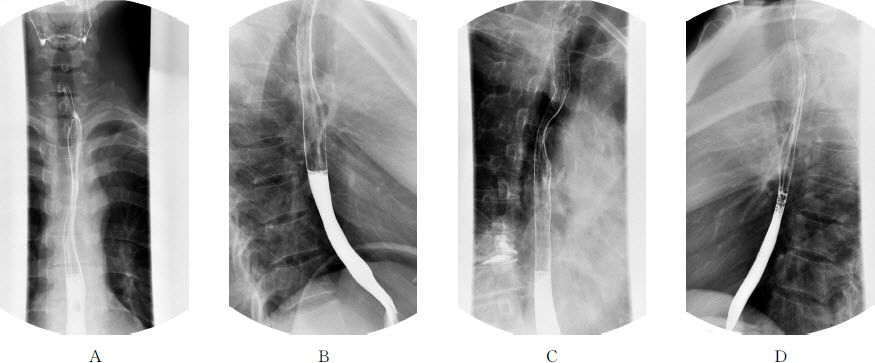
\includegraphics{./images/Image00233.jpg}
 \captionsetup{justification=centering}
 \caption{食管钡餐造影片}
 \label{fig5-1-1}
  \end{figure} 

\textbf{【X线诊断】}  正常食管钡餐片。

\begin{figure}[!htbp]
 \centering
 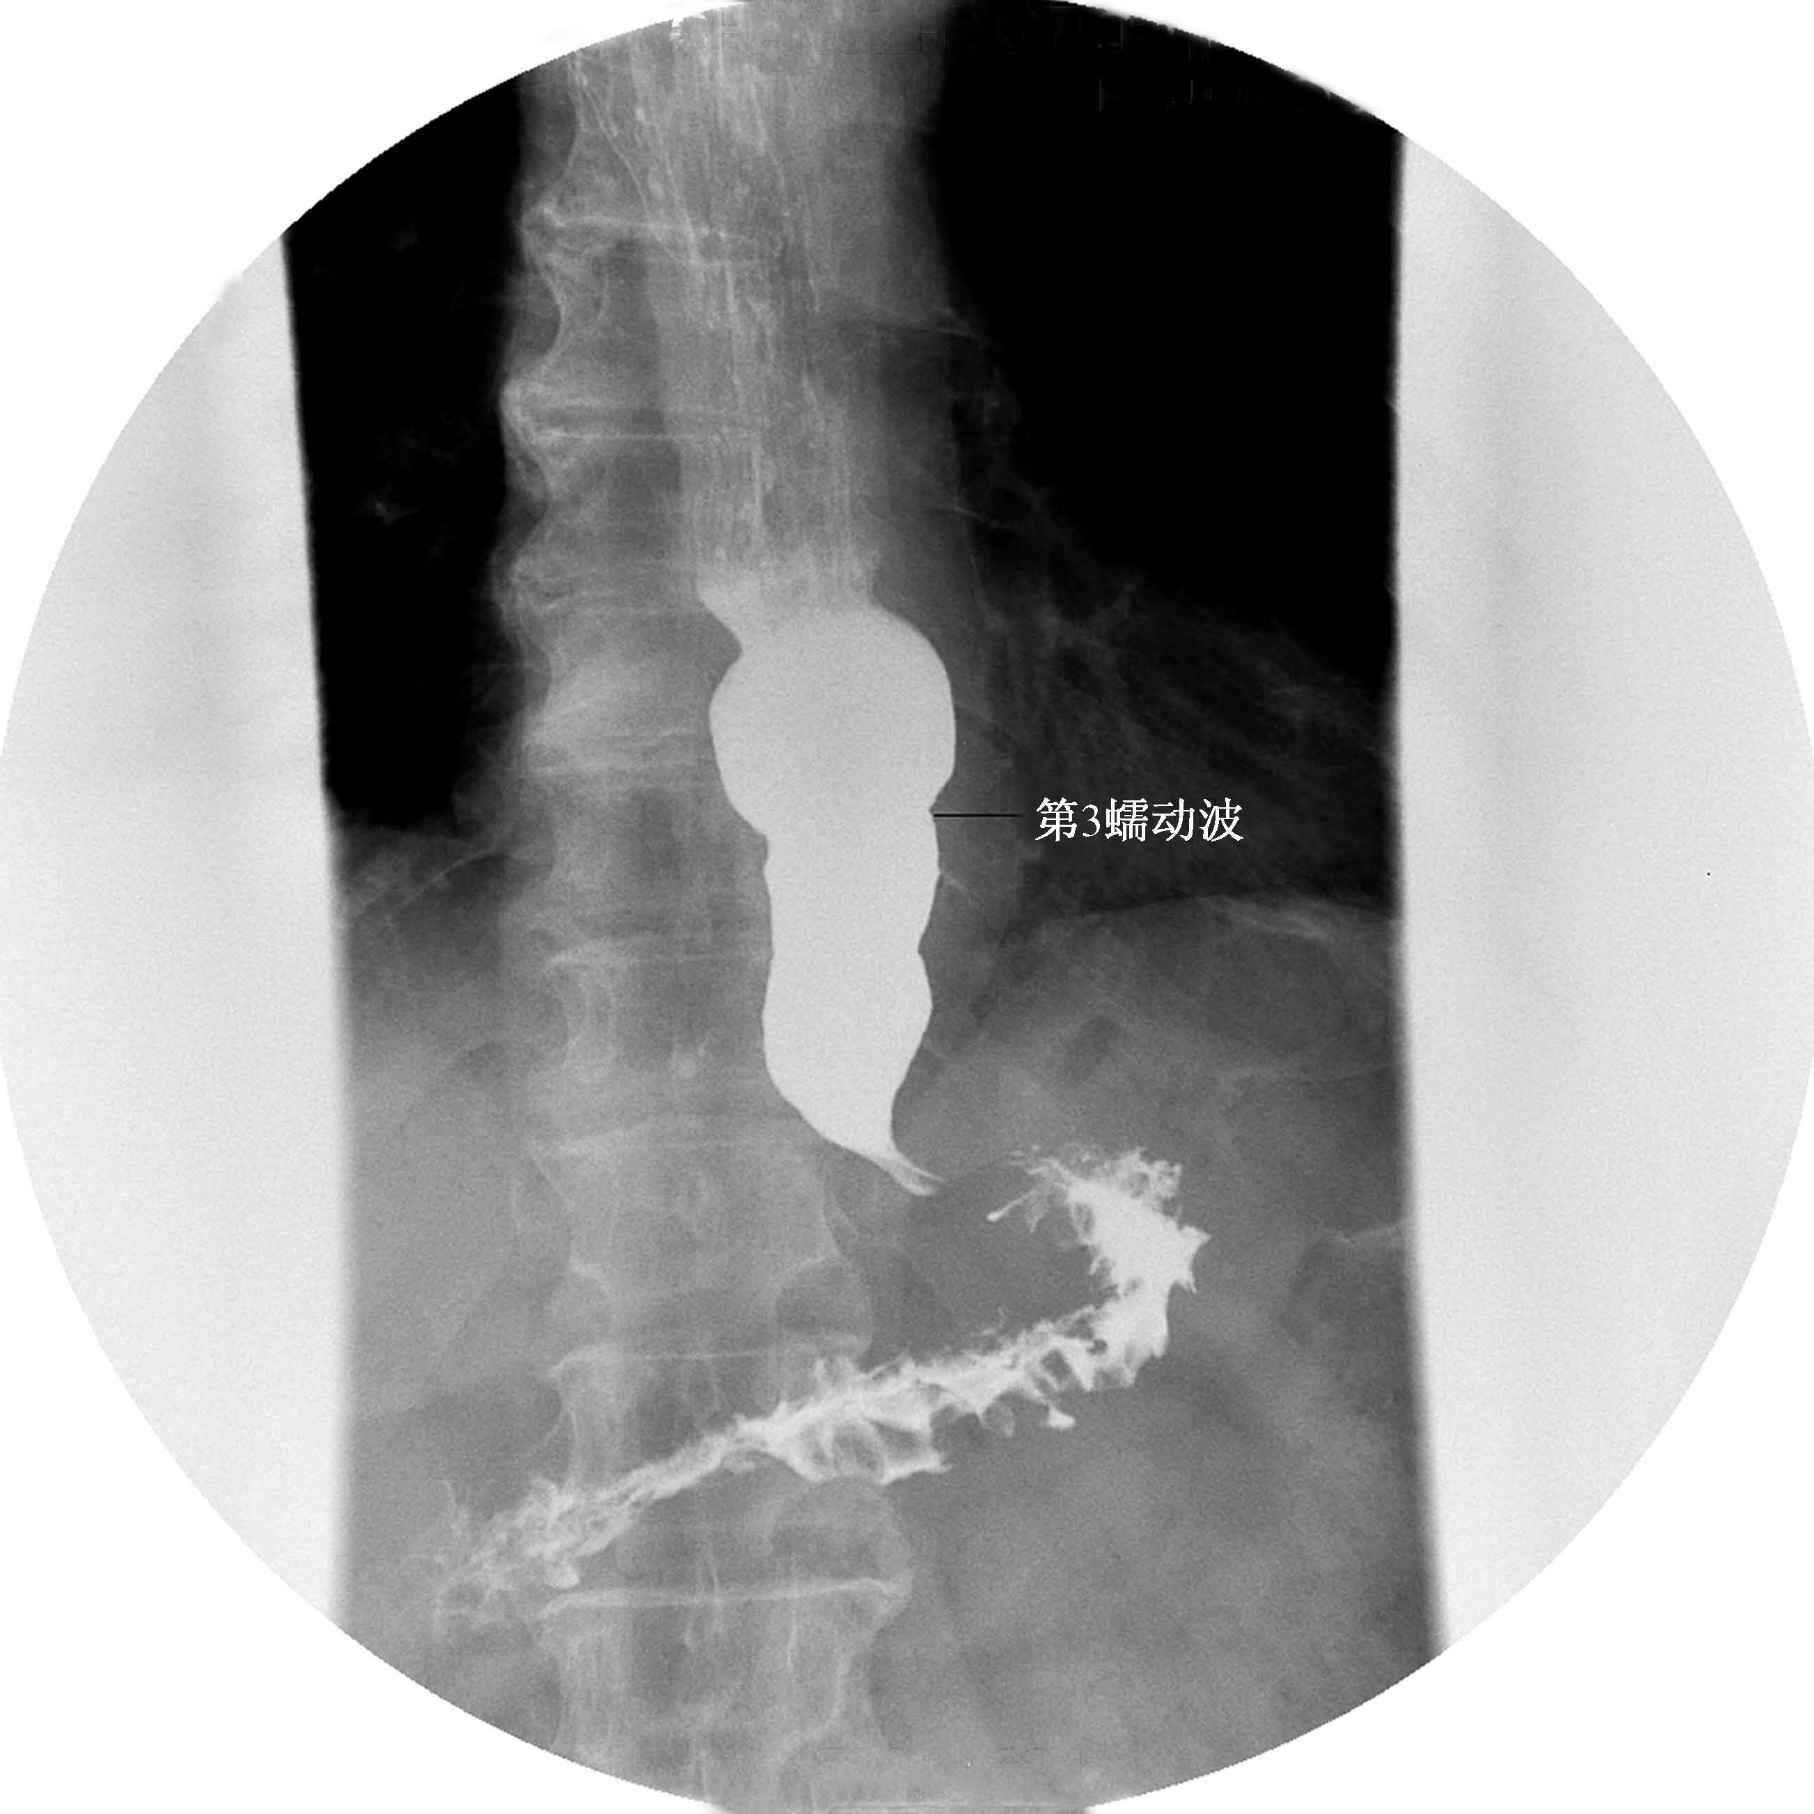
\includegraphics{./images/Image00234.jpg}
 \captionsetup{justification=centering}
 \caption{食管第3蠕动波}
 \label{fig5-1-2}
  \end{figure} 

\textbf{【X线表现】}
 所谓第3蠕动波是食管环状肌的局限性不规则收缩运动,形成波浪状或锯齿状边缘,出现突然,消失迅速,多发于食管下段,常见老年人和食管贲门失迟缓症者。

\textbf{【X线诊断】}  食管贲门失迟缓症;食管第3蠕动波。

\begin{figure}[!htbp]
 \centering
 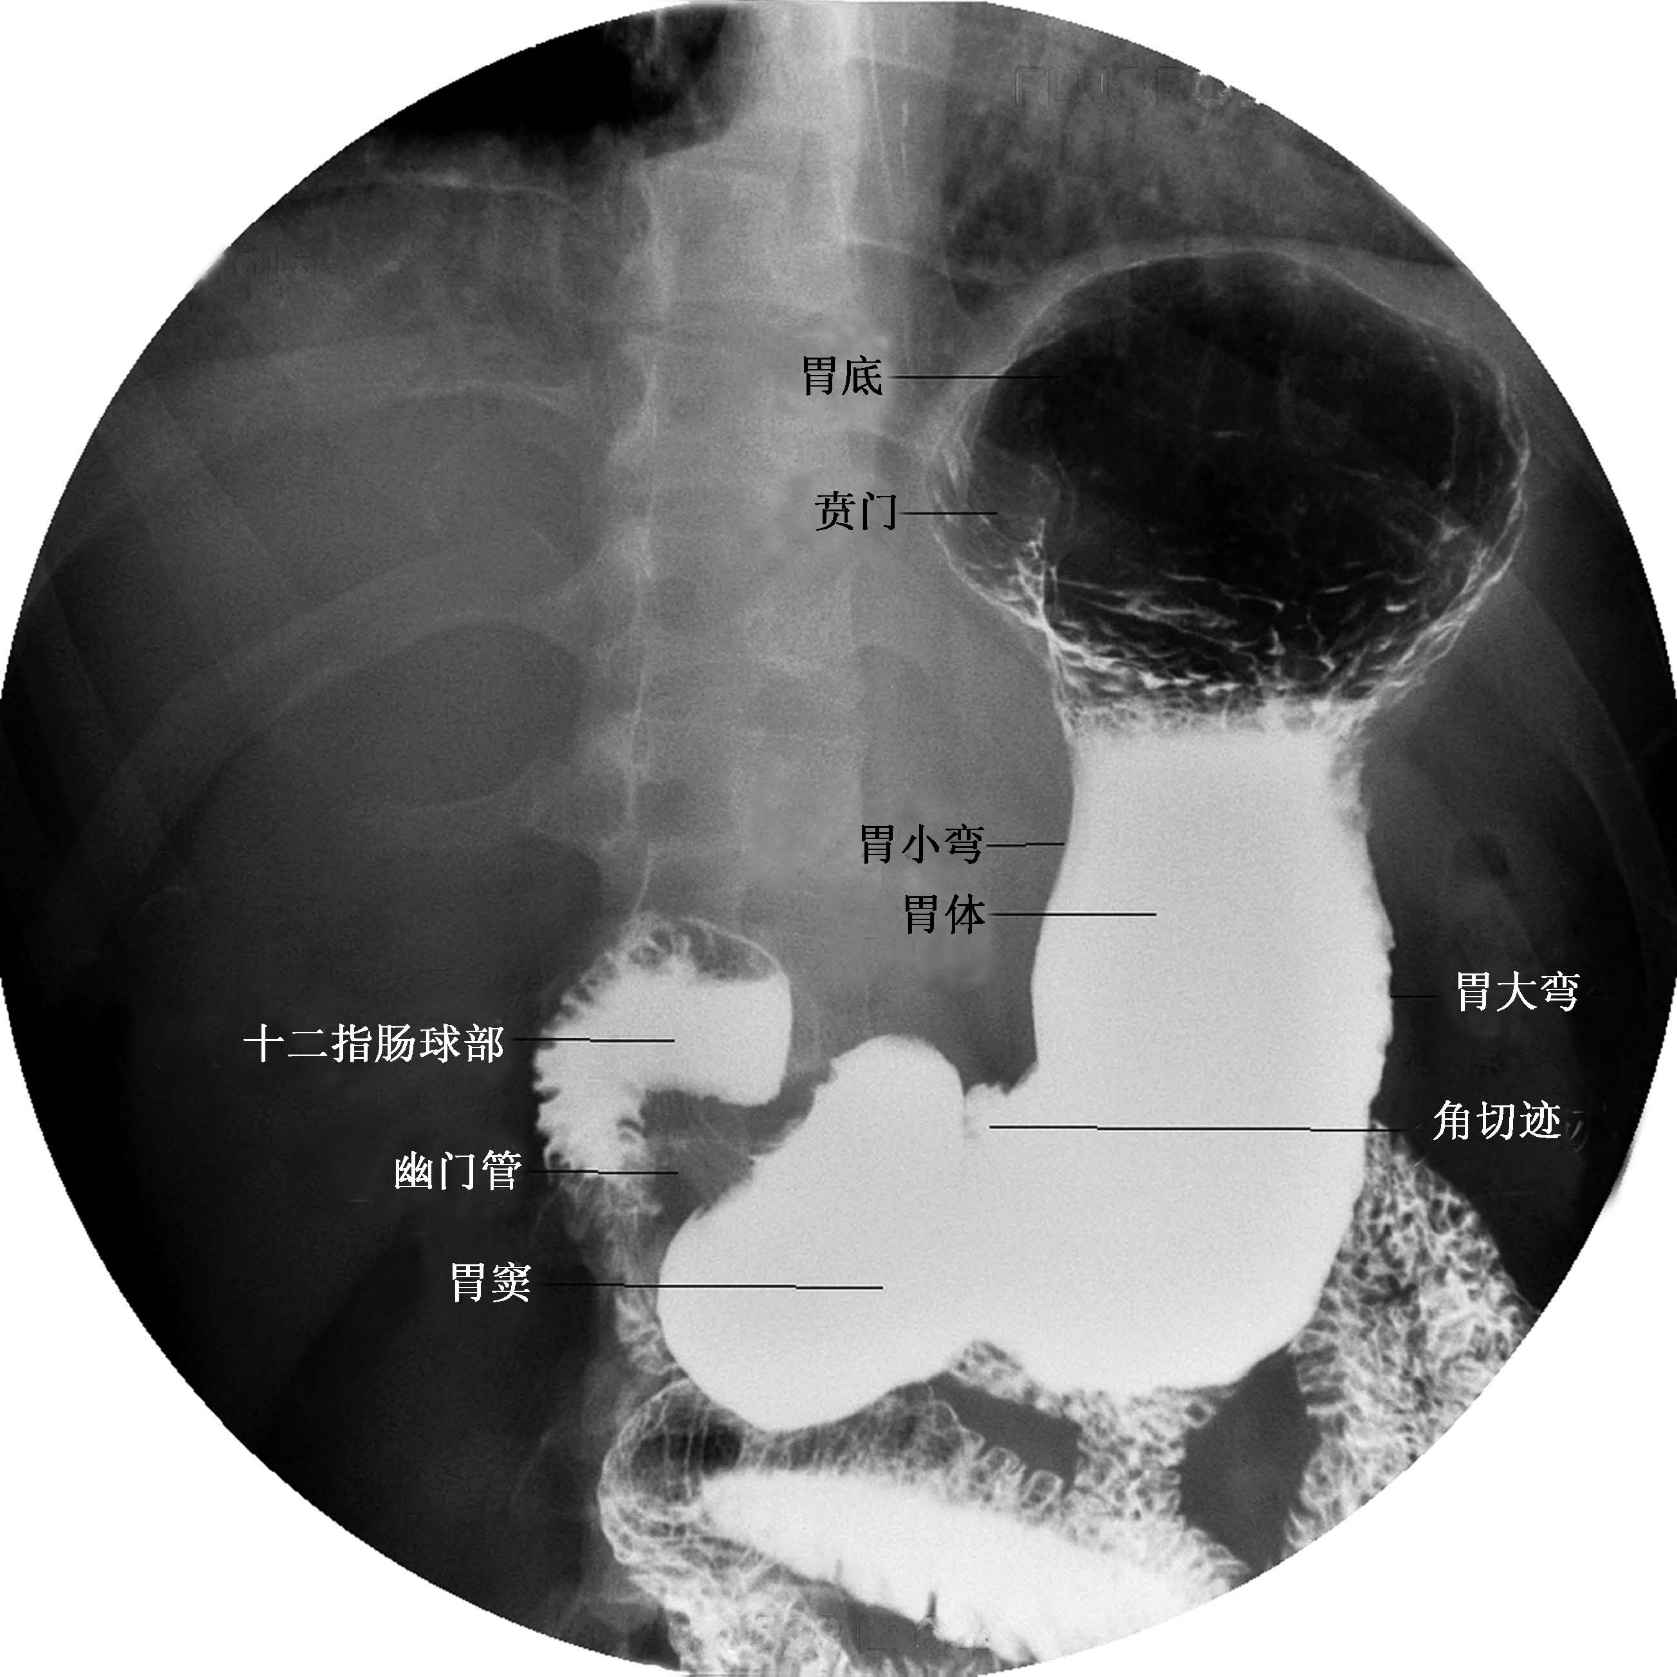
\includegraphics{./images/Image00235.jpg}
 \captionsetup{justification=centering}
 \caption{胃的X线解剖部位划分及命名}
 \label{fig5-1-3}
  \end{figure} 

(1)贲门:食管进入胃的开口处。

(2)胃底:贲门横线以上区域。

(3)贲门区:以贲门为中心,半径约为2.5cm的圆形区域。

(4)胃小弯:胃的右上侧边缘。

(5)胃大弯:胃的左外下侧边缘。

(6)胃角(角切迹):胃小弯转折处。

(7)胃窦:角切迹与胃大弯最低点连线与幽门之间的区域。

(8)胃体:胃窦与胃底之间的区域。

(9)幽门管:胃部通向十二指肠球部的细短管状结构。

\begin{figure}[!htbp]
 \centering
 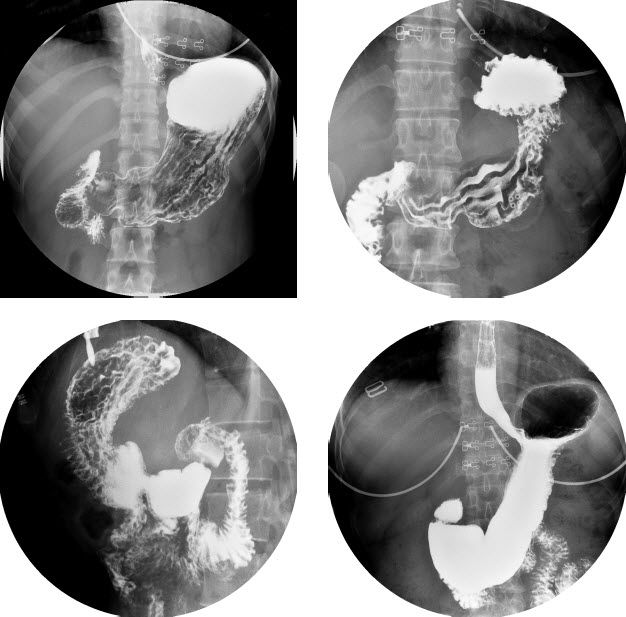
\includegraphics{./images/Image00236.jpg}
 \captionsetup{justification=centering}
 \caption{胃钡餐造影片}
 \label{fig5-1-4}
  \end{figure} 

\textbf{【X线表现】}
 胃的轮廓在胃小弯侧及胃窦大弯侧光滑整齐,胃体大弯侧呈锯齿状,系横、斜走行的粘膜皱襞所致。

胃的粘膜皱襞像,可见皱襞间沟内充以钡剂,呈致密的条纹状影。皱襞则显示为条状透亮影。胃小弯侧的皱襞平行整齐,一般可见3~5条,平均宽约0.5cm。角切迹以后,一部分沿胃小弯走向胃窦,一部分呈扇形分布,斜向大弯。胃体大弯侧的粘膜皱襞为楔形、横行而呈不规则的锯齿状,宽0.2~0.4cm,大于0.5cm为异常表现。胃底部粘膜皱襞排列不规则,相互交错呈网状。胃窦部的粘膜皱襞可为纵行、斜行及横行,收缩时为纵行,舒张时以横行为主,排列不规则。

\textbf{【X线诊断】}  正常胃的粘膜皱襞。

\begin{figure}[!htbp]
 \centering
 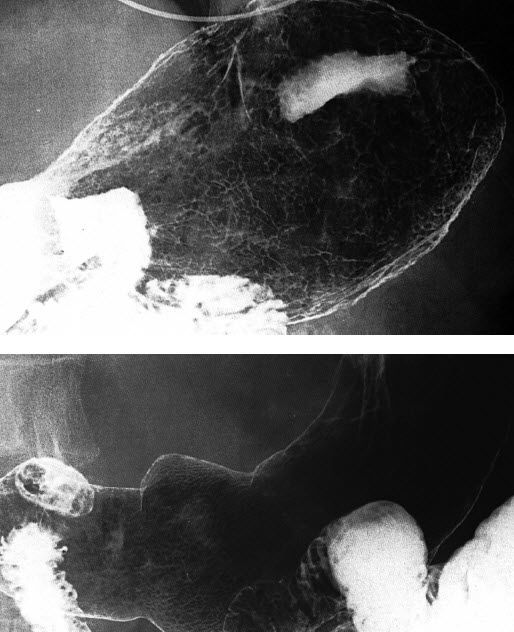
\includegraphics{./images/Image00237.jpg}
 \captionsetup{justification=centering}
 \caption{胃双对比造影片}
 \label{fig5-1-5}
  \end{figure} 

\textbf{【X线表现】}
 胃的双对比造影显示粘膜皱襞的细微结构即胃小区、胃小沟。正常胃小区为1~3mm大小,呈圆形、椭圆形或多角形大小相似的小隆起,其由于钡剂残留在周围浅细的胃小沟而显示出,呈细网眼状。正常的胃小沟粗细一致,轮廓整齐,密度淡而均匀,宽约1mm以下。

\textbf{【X线诊断】}  正常胃小区。

\textbf{【临床经验】}
 应当强调,X线征象的显示情况与检查方法有密切的关系。近年来,由于开展了气钡双重造影,对于龛影形态及胃粘膜皱襞的显示提供了良好的条件。临床工作中,只有把充盈像、粘膜皱襞像及粘膜像结合起来,才能比较确实地反映出龛影的病理形态。在良、恶性溃疡鉴别诊断时,良性胃溃疡多数表现为龛周胃小沟纤细,胃小区多数显示不清,少数显示形态不规则。另有见龛周胃小沟粗细不均,胃小区显示清晰,但形态不规则,呈多样性改变。恶性胃溃疡龛周胃小沟、胃小区破坏,癌组织代替了正常粘膜层,呈多样性改变。如结节样、磨砂玻璃样以及条索状,部分病例在靠近正常粘膜区,胃小区尚可辨认,但胃小沟粗细不均、紊乱、破坏。所以我们认为,龛周胃小区改变呈萎缩型或增生型者为良性溃疡;龛周胃小区呈破坏型代之以结节状、磨砂玻璃状、不规则条状皱襞改变者为恶性溃疡。

\begin{figure}[!htbp]
 \centering
 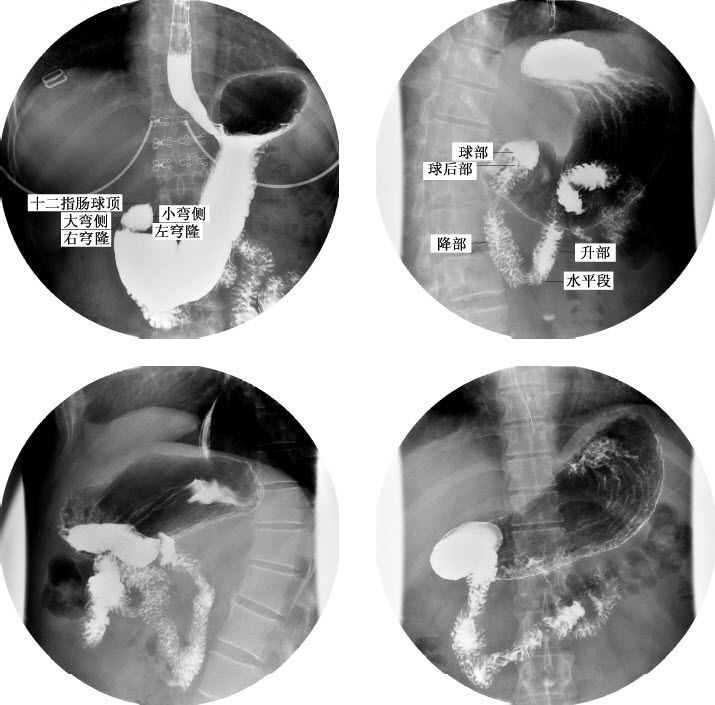
\includegraphics{./images/Image00238.jpg}
 \captionsetup{justification=centering}
 \caption{上消化道钡餐造影片}
 \label{fig5-1-6}
  \end{figure} 

\textbf{【X线表现】}
 十二指肠全程称十二指肠曲,因其成半环形又称为十二指肠环。一般分为球部、降部、水平部和升部。球部:充盈时呈边缘整齐的三角形,尖部指向右上后方,底部平整,两侧有对称的隐窝,幽门开口于球底中央。球尖顶到降部之间的一小段,X线上称为球后部,其长短不一,一般可达4~5cm,短时几乎不存在。粘膜皱襞可呈纵行,有4~5条,也可呈横行或花纹状,在双重造影时,球部粘膜可呈细网状或小点状,为粘膜绒毛及绒毛间沟充钡所致。球部充盈不全时,其边缘可不规则,为粘膜皱襞所致,易误为异常。因球部及球后部向右后方,所以,右前斜位便于观其全貌,左前斜位便于球部前后壁的显示。降部、水平部、升部:充盈后内外缘对称,因粘膜皱襞的影响,两侧缘呈锯齿状,尤以外缘明显,粘膜皱襞呈环形或羽毛状,收缩时则成纵行。蠕动呈波浪状前进,并可见逆蠕动,不能误为异常。降部宽2~3cm。十二指肠双重造影时,管径可增加一倍,羽毛状粘膜皱襞消失,代之以环形或龟背状花纹,或二者兼有。降部内缘可较平直或略凸,中段可见一肩样突起,称为岬部,其下方较平直,可见纵行皱襞。十二指肠乳头在岬部下方,呈圆形或类圆形,边界清晰,直径一般不超过1.5cm。乳头开口处可存钡,表现为点状,为正常现象。在乳头影上方有时可见一直径数毫米的圆形透亮区,为副乳头。

\textbf{【X线诊断】}  十二指肠正常X线表现。

\begin{figure}[!htbp]
 \centering
 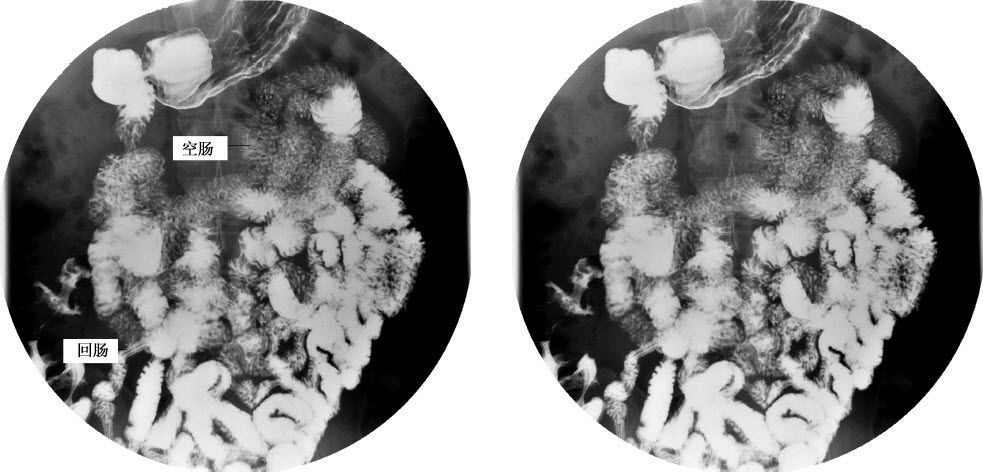
\includegraphics{./images/Image00239.jpg}
 \captionsetup{justification=centering}
 \caption{小肠钡餐造影片}
 \label{fig5-1-7}
  \end{figure} 

\textbf{【X线表现】}
 平片检查,正常成人的小肠内虽有气体,但与食糜混合存在,而不能显示。长期卧床、幼儿及肠紧张的老年人,小肠内有分散的气团,多见于腹中部,为正常表现。另外,患者由卧位改成立位检查时,十二指肠球部可有积气,不能误为异常。造影检查,小肠长度平均为280cm,其长度与体重关系明显,与身长关系不明。空回肠两端较固定,其余部分活动度较大。空肠居于左上腹及中腹部,回肠位于右下腹及盆腔。一般上部肠曲多横行,下部肠曲多纵行。空肠管径较大,为2.5~3cm,回肠管径1.5~2.5cm。空肠粘膜呈细羽毛状,其长短、粗细、形态和方向随肠壁肌张力而变化。收缩时呈纵行状,舒张时呈环形,粘膜面仅有少量钡餐附着时,则呈雪花状。回肠粘膜皱襞则稀疏、低平而不明显,其末端常呈纵行皱襞。在小儿,由于淋巴组织丰富,淋巴集结可呈卵石状,多见于回肠。小肠运动主要为蠕动,表现为节段性充盈与排空。空肠蠕动迅速有力,回肠慢而弱,但分节运动较明显,表现为节律性收缩与舒张。小肠的运动受胃内钡剂排出状况影响,胃蠕动强、排出量大时,小肠的运动也增强。常规口服钡餐造影时,钡剂到达回盲瓣的时间一般为2~6小时,7~9小时钡剂从小肠全部排空。老年人排空时间延缓,可达11小时。如果少于1小时钡剂到达盲肠,为运动增快,超过6小时则为运动过缓。为了便于X线检查的描述,按小肠位置将其分为六组:①十二指肠。②上部空肠,位于左上腹部。③下部空肠,位于左腹部。④上部回肠,位于右中腹部。⑤中间回肠,位于右中下腹部。⑥下部回肠,位于盆腔内。

\textbf{【X线诊断】}  小肠正常X线表现。

\begin{figure}[!htbp]
 \centering
 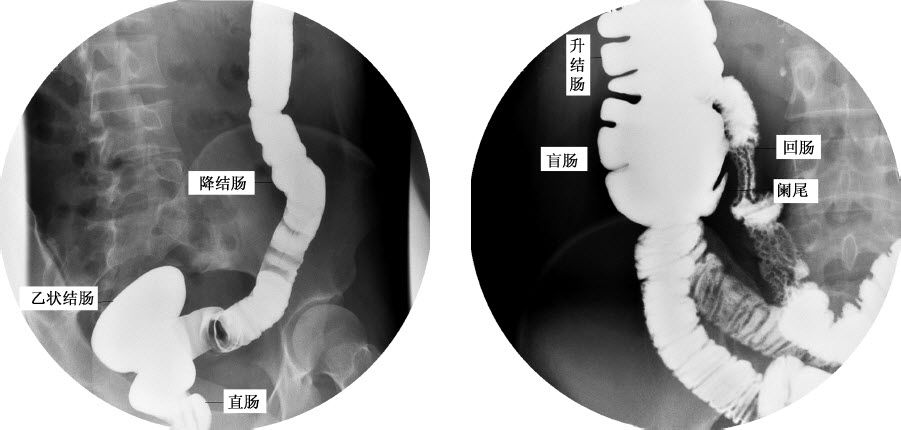
\includegraphics{./images/Image00240.jpg}
 \captionsetup{justification=centering}
 \caption{结肠钡剂造影片}
 \label{fig5-1-8}
  \end{figure} 

\begin{figure}[!htbp]
 \centering
 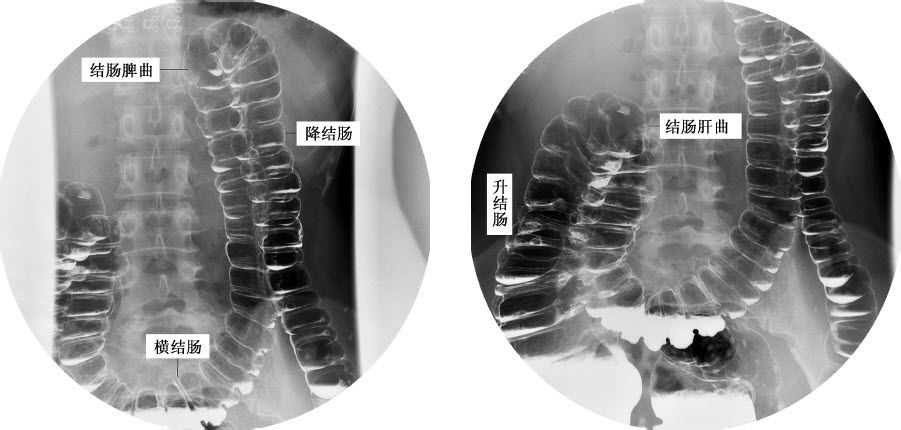
\includegraphics{./images/Image00241.jpg}
 \captionsetup{justification=centering}
 \caption{结肠气钡双重造影}
 \label{fig5-1-9}
  \end{figure} 

\textbf{【X线表现】}
 盲肠位于右髂窝内,移动度较大,故位置不固定,可高至肝下或低至盆腔,甚至到左下腹部,但一般移动范围在10cm左右。回盲瓣开口于盲肠后内侧壁,上唇较长约2cm。下唇约0.6cm,瓣口为圆形、椭圆形或呈横裂口。阑尾一般位于盲肠下内侧,钡剂造影显示率为60%,充盈时光滑整齐,活动度大,有时可见粪石形成的充盈缺损,阑尾多与盲肠同时排空或稍延缓。横结肠和乙状结肠的系膜较长,因此,活动范围较大,其余部分位置较固定。直肠壶腹部内径最大,盲肠次之、盲肠向远端逐渐变窄,乙状结肠与直肠移行处最窄,为2~3cm,勿误为病理表现。常规钡剂灌肠时,因生理括约肌的作用,在回盲瓣的对侧、升结肠、横结肠近端和远端、降结肠下部、乙状结肠等部位,可见肠腔局限性狭窄,不能误为异常。

结肠的粘膜皱襞有横、纵、斜三个方向相互交错。盲肠、升结肠及横结肠的粘膜皱襞较显著,降结肠及其远段则稀疏。环肌收缩时粘膜呈纵行皱襞。

直肠没有结肠袋,但直肠壶腹的前壁及侧壁可见半圆襞形成的切迹。直肠后壁与骶骨之间称骶骨前间隙或称直肠后间隙,测量方法是第3~5骶骨前缘到直肠后壁的最短距离,而以第5骶骨处测量较准确。约95%的正常人此间隙小于或等于0.5cm,大于1.5cm时可疑异常,大于2cm者为病理性增大。

双重造影时,结肠的轮廓呈连续、均匀的线条,粗约1mm。其微小皱襞称无名线,此乃结肠的基本解剖单位,切线位表现为微细的刺状突出,深约0.2mm。正面观为0.1~0.2mm,并以0.6~1mm的间距与肠壁垂直分布,或交织呈网状。良好的双重造影片上,无名线的显示率可达90%。在结肠排空像的边缘有时可见深0.5~2mm、粗1mm、以3~5mm间距分布的尖刺影,称边缘锯齿征,或称结肠假溃疡征,是钡剂嵌于结肠Lieberkuhns腺管腺窝所致,出现率为5%~10%。复查时可消失,为正常表现。

\textbf{【X线诊断】}  正常结肠造影片。

\begin{figure}[!htbp]
 \centering
 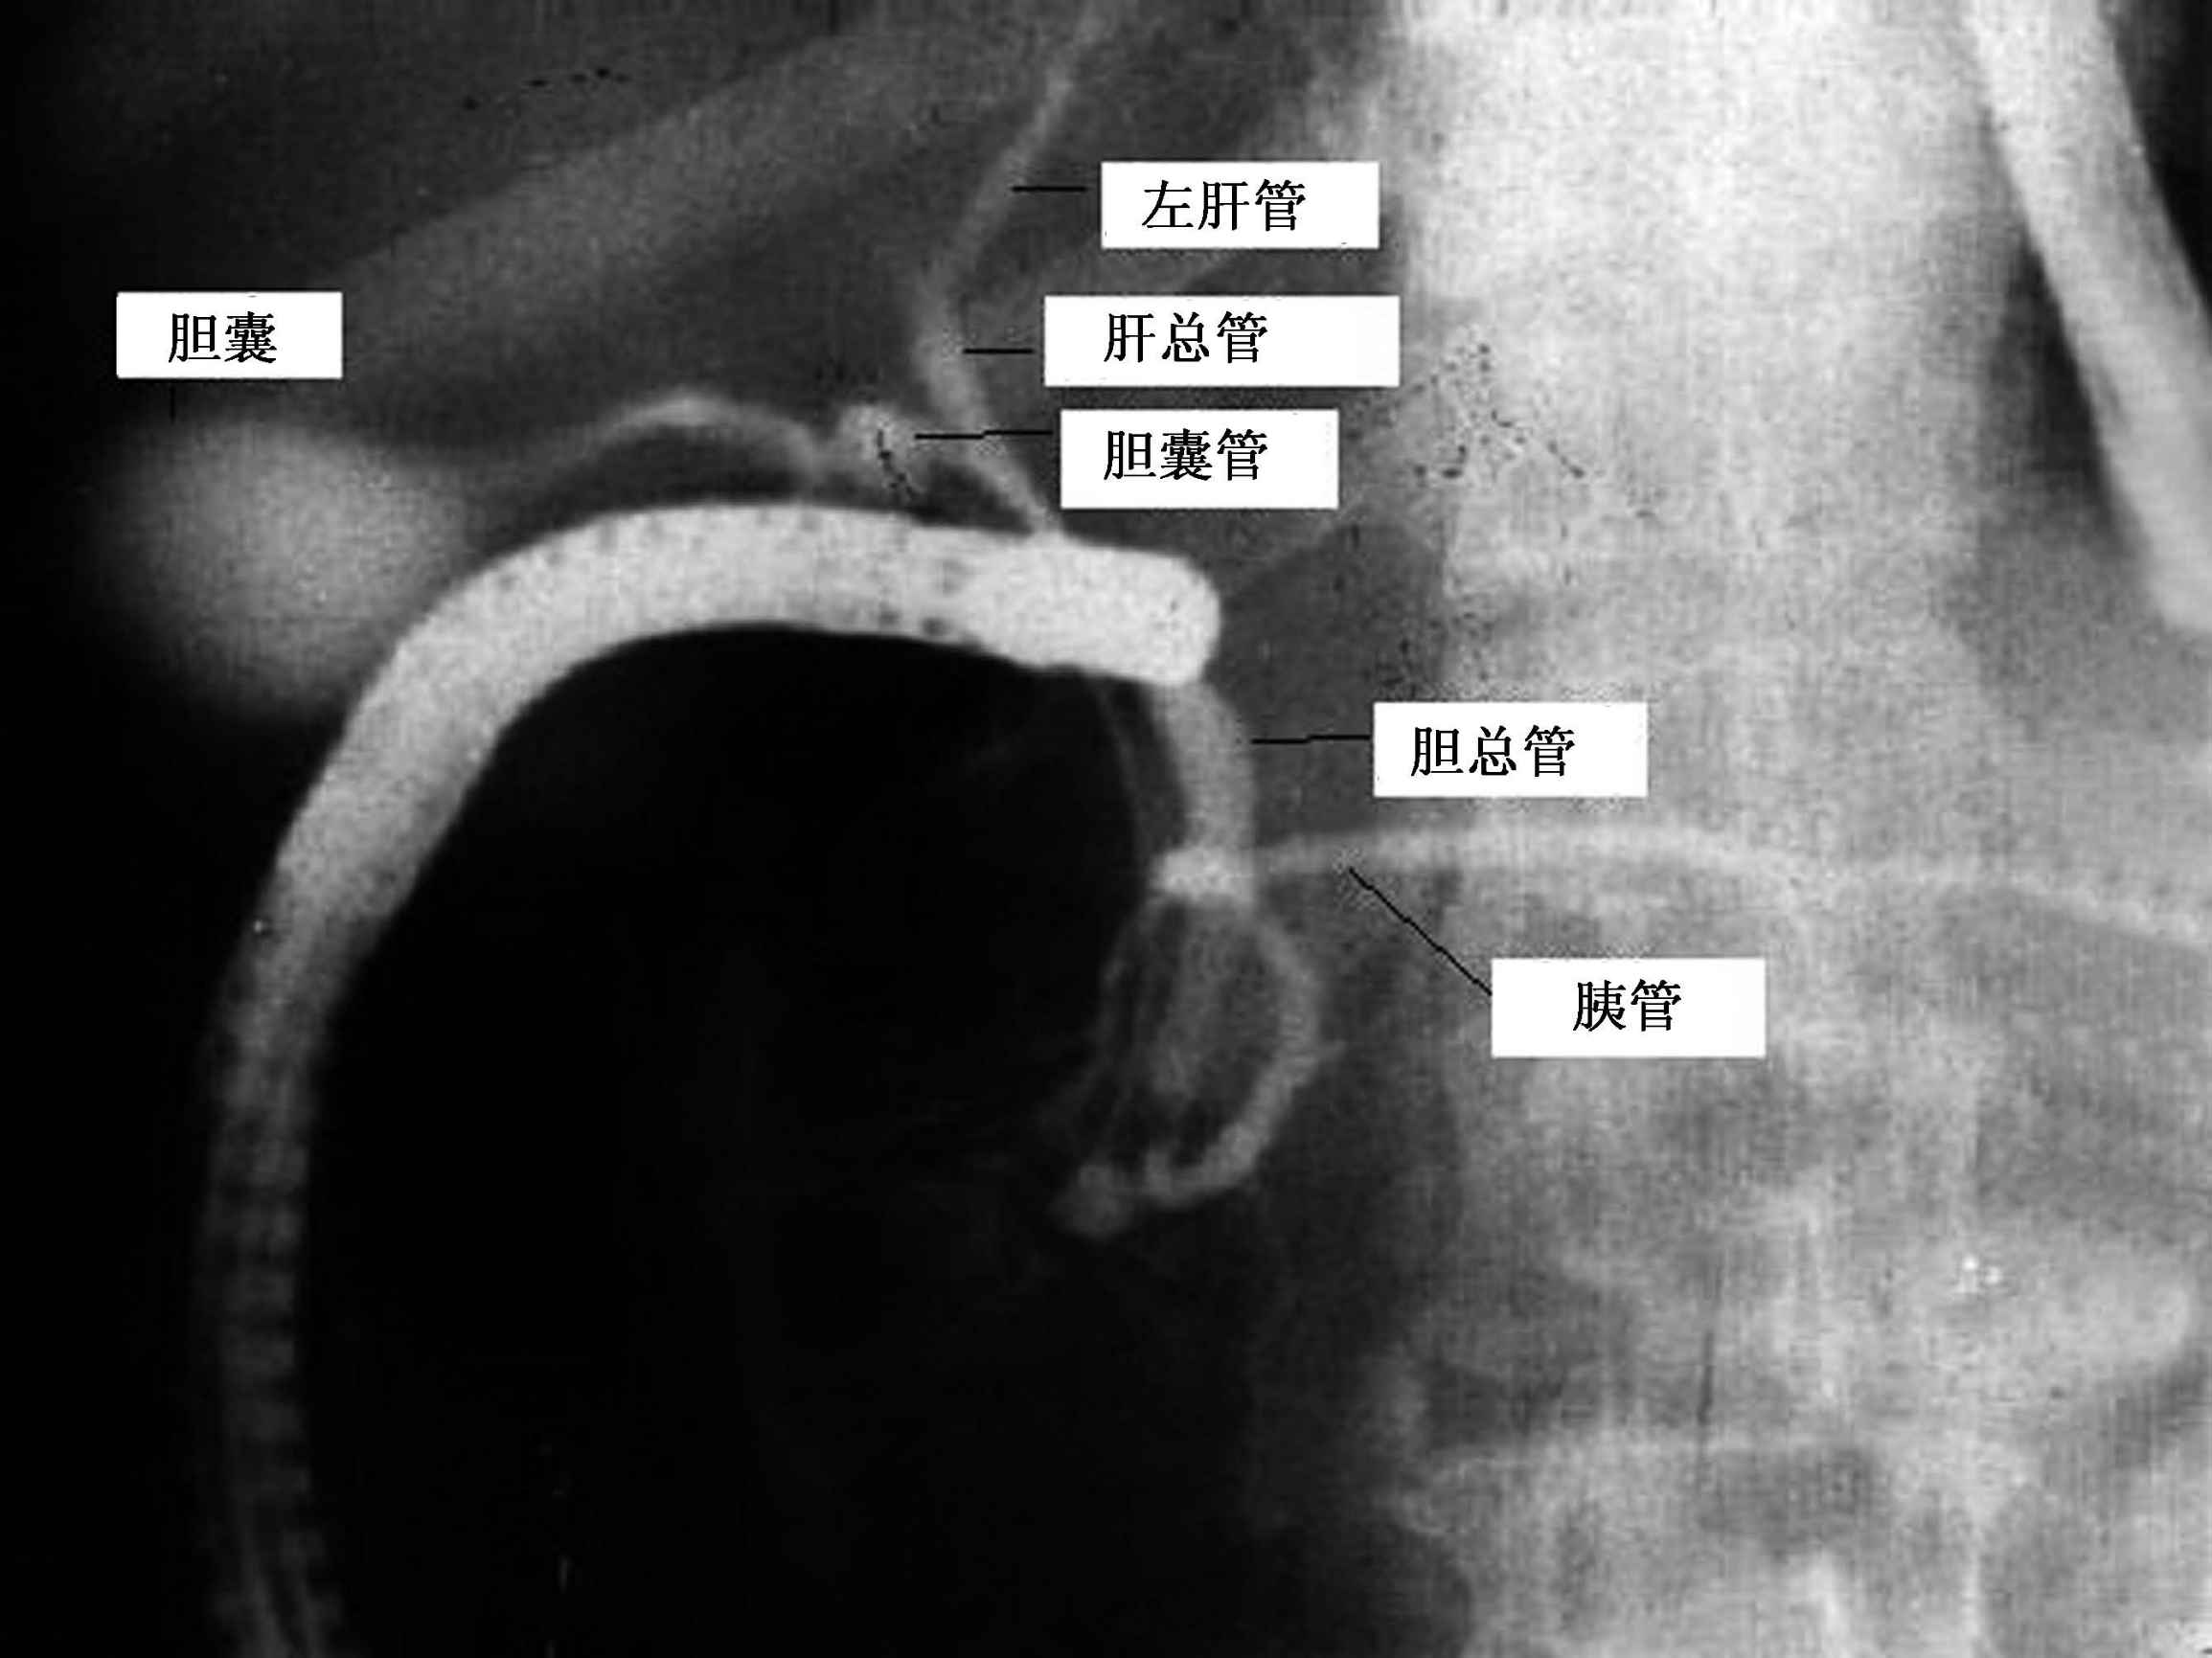
\includegraphics{./images/Image00242.jpg}
 \captionsetup{justification=centering}
 \caption{经内镜逆行胰胆管造影片}
 \label{fig5-1-10}
  \end{figure} 

\textbf{【X线表现】}
 胆囊大小、形态、位置因人的体质及体位不同而不同,一般分为梨形、圆形和长形三种,最常见为梨形,长7~10cm,宽3~4cm,形态上胆囊可分为底部、体部、漏斗部和颈部。胆管分肝内胆管和肝外胆管两部分,肝内胆管由左、右肝管及其分支组成,肝外胆管由肝总管、胆囊管和胆总管组成。肝总管长3~4cm,宽5~6mm;胆囊管长3~4cm,宽2~3mm;胆总管长7~8cm,宽5~6mm。胆总管穿过十二指肠壁,终止于十二指肠大乳头,构成肝胰壶腹(Oddi)括约肌,宽12mm,长约数毫米,在其上方略为膨大成为肝胰壶腹,胰管汇合于此。

\textbf{【X线诊断】}  胆道系统正常X线表现。

\begin{figure}[!htbp]
 \centering
 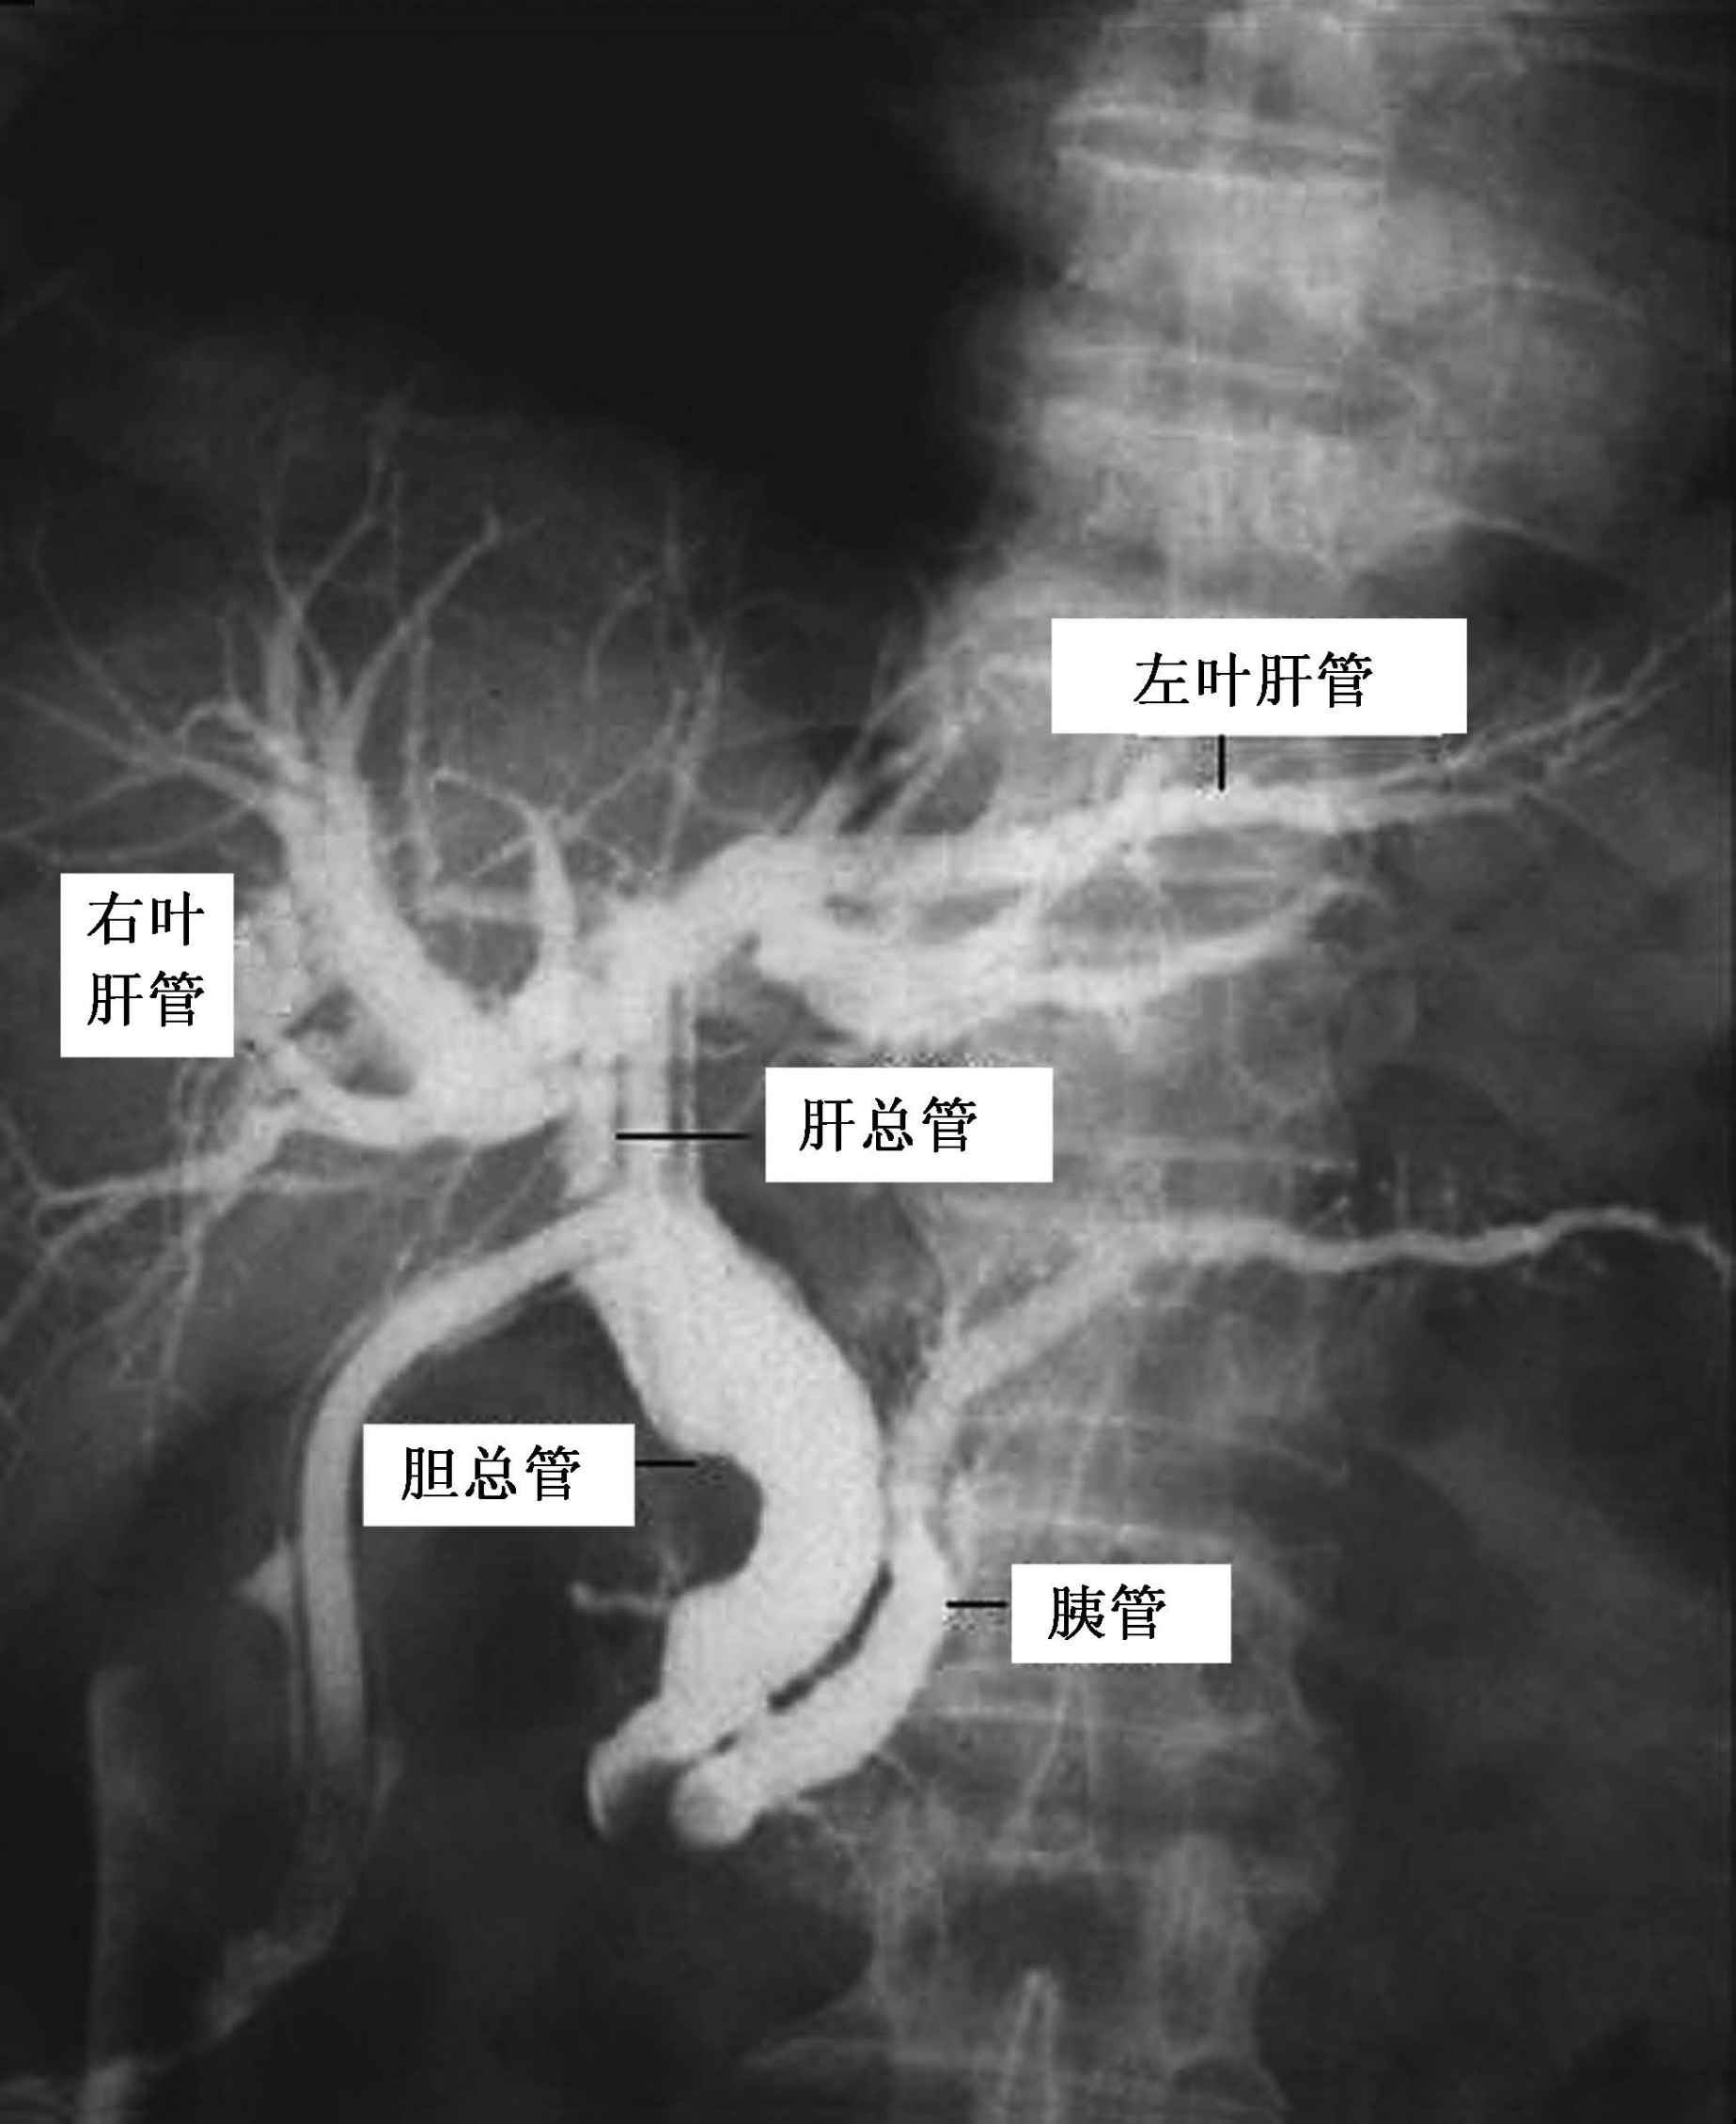
\includegraphics{./images/Image00243.jpg}
 \captionsetup{justification=centering}
 \caption{T管造影片}
 \label{fig5-1-11}
  \end{figure} 

\textbf{【X线表现】}
 胰腺管分为主胰管和副胰管,主胰管从十二指肠大乳头开始,多为从右下斜行向左上,或呈横行、乙字形走行于第12胸椎至第2腰椎水平之间。主胰管分为头部、体部和尾部,全长14~18cm;宽:头部4mm,体部3mm,尾部2mm。副胰管于主胰管的头、体交界处与主胰管汇合,大致呈水平走向于十二指肠壁开口于十二指肠小乳头。

\textbf{【X线诊断】}  肝内外胆管及胰腺管X线解剖。

\section{食管病变}

\subsection{食管金属异物}

\begin{figure}[!htbp]
 \centering
 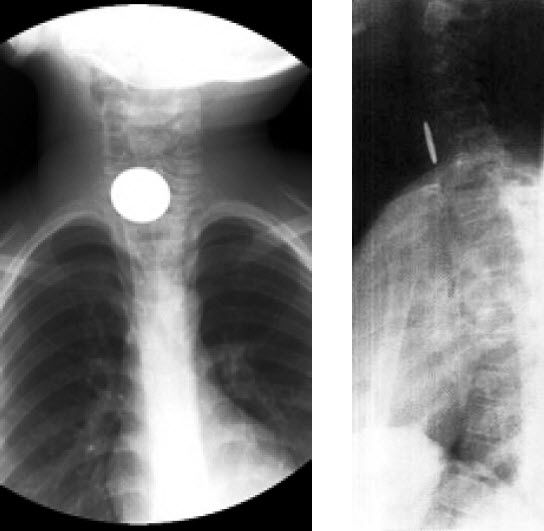
\includegraphics{./images/Image00244.jpg}
 \captionsetup{justification=centering}
 \caption{颈胸部正侧位片}
 \label{fig5-2-1}
  \end{figure} 

\textbf{【病史摘要】}
 男性,3岁。玩耍时不慎将1元硬币吞下,烦躁、哭闹1小时。自述吞咽不适。

\textbf{【X线表现】}  第7颈椎水平见一直径约2.0cm大小圆形不透光异物影。

\textbf{【X线诊断】}  食管入口处金属异物。

\textbf{【评  述】}
 依据患儿有明确的误吞金属异物病史,故常规的透视和颈胸部食管正侧位摄片即可观察到异物的形态,确定异物的位置,不需钡餐造影,诊断一般不会发生困难。需注意的是颈胸部的钙化影和气管内异物有时与食管内不透光异物相似,食管异物在侧位片上,位于气管之后,长形异物与食管纵轴一致;扁平形异物正位呈片状,侧位呈条状,而气管异物恰与此相反。异物最易滞留于食管生理狭窄和压迹处,故应重点观察,尤以食管入口(管径最小)为主,对于滞留于非好发部位的异物,应警惕食管器质性病变的可能性。有时食管内异物在患者的强力吞咽动作下,食管的生理狭窄和压迹处也可以充分扩张,使食管异物通过全食管抵达胃部,甚至肠道,所以在临床工作中,如果怀疑有异物存在,颈胸部X线检查未发现异物时,应进一步检查胃肠道,观察异物是否自行咽下,这是我们要注意的地方。

\subsection{食管透光性异物}

\begin{figure}[!htbp]
 \centering
 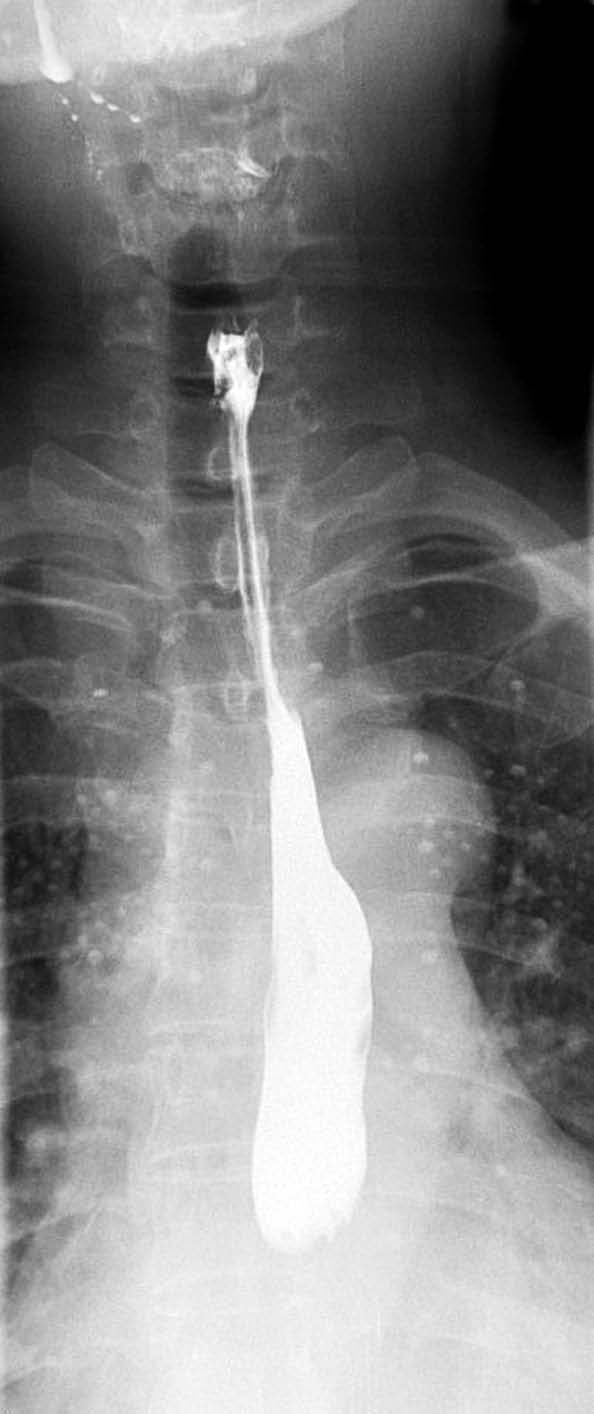
\includegraphics{./images/Image00245.jpg}
 \captionsetup{justification=centering}
 \caption{钡棉造影检查}
 \label{fig5-2-2}
  \end{figure} 

\textbf{【病史摘要】}
 男性,50岁。1小时前喝鱼汤时误将鱼刺咽下,感咽部疼痛,吞咽有异物感。

\textbf{【X线表现】}
 钡棉透视示钡棉滞留于食管上段平第6颈椎水平无法下行,未显示异物的形态。

\textbf{【X线诊断】}  食管上段透光异物(鱼刺)。

\textbf{【评  述】}
 对于较小的食管异物或是不透X线的异物时,应行钡棉造影检查,钡棉往往能停挂在异物处,嘱咐患者反复吞咽甚至饮水钡棉仍能停留在原处,称为挂絮征象,可以对细小异物做出诊断,也是对不透X线异物检查的有效方法,小的透光异物,如鱼刺、小骨片等一般常规透视和摄片检查不易发现,简单的钡餐透视亦不能显示。过小、过细的骨和鱼刺或嵌入咽或食管较深外露于粘膜面较小的异物不易显示挂絮征象,异物损伤了咽或食管的粘膜,患者的自觉症状也难以与异物滞留鉴别,拟建议内镜检查。

钡棉造影检查中需要重点注意的是:①当怀疑异物在主动脉弓水平附近而又需钡棉检查才能确定时,此时应以少量多次吞服钡棉为好,如一次性吞服大量钡剂有可能会牵引异物而致使食管穿孔,甚至累及大血管而致大出血,危及患者生命。②如患者吞服异物时间较长,在透视或摄片中见到异物处食管周围软组织肿胀甚至出现气液平面,则提示食管异物处有炎症感染或脓肿形成,此时吞钡检查会出现钡剂外溢现象且不能排空。

\subsection{反流性食管炎}

\begin{figure}[!htbp]
 \centering
 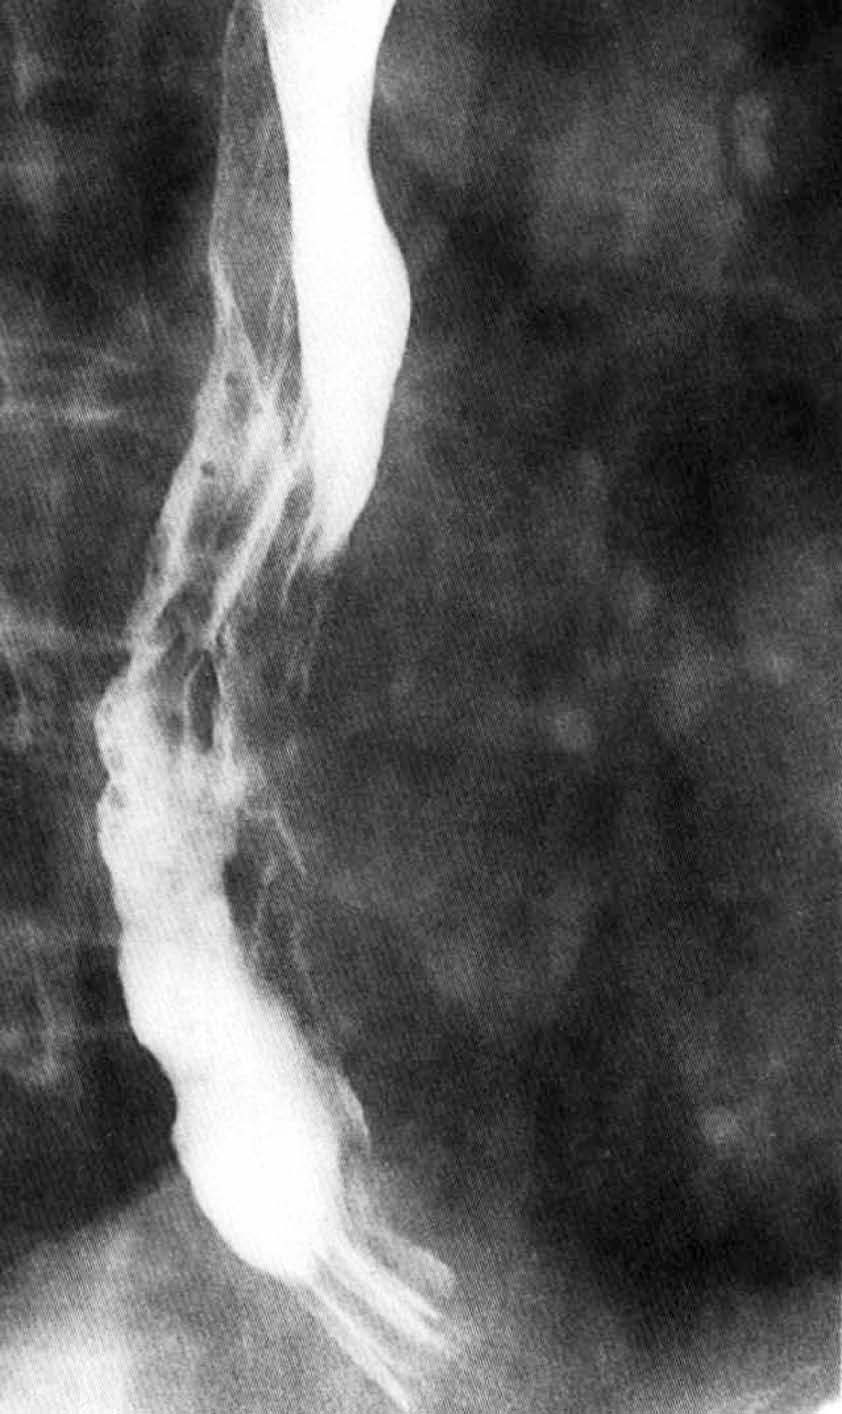
\includegraphics{./images/Image00246.jpg}
 \captionsetup{justification=centering}
 \caption{反流性食管炎}
 \label{fig5-2-3}
  \end{figure} 

\textbf{【病史摘要】}
 男性,55岁。胸骨后及心窝处烧灼感及疼痛,进食尤其是进热食疼痛加剧,卧位或弯腰时加重,有轻度吞咽困难。

\textbf{【X线表现】}
 右前斜卧位片示:食管内大量钡剂反流,中下段粘膜增粗、紊乱,内见小颗粒征,粘膜未见中断破坏。

\textbf{【X线诊断】}  反流性食管炎。

\textbf{【评  述】}
 X线为检查食管炎症重要的方法,造影检查与内镜证实的符合率可达90%以上,尤其对于中晚期病例。检查中应充盈法、粘膜法和低张双对比造影法相结合,还要应用多种体位及增加腹压等措施。早期可仅见功能异常,表现为吞咽激发的原发性蠕动到主动脉弓水平处终止或减弱,胃食管反流致中下段痉挛性狭窄,狭窄段可有蠕动,钡剂通过时可扩张,通过后又重复出现,但形态不固定、与癌性浸润不同。或者粘膜呈颗粒状,颗粒为1~2mm。表浅溃疡则呈小针刺状龛影。在后期,因瘢痕收缩,而致永久性无明显分界的狭窄及短缩,狭窄段一般4~5cm,多数规则、光滑,也可因瘢痕收缩牵引而不规则,呈假憩室状,低张双重造影显示较好。食管短缩者可见牵引性裂孔疝。发现痉挛性狭窄时,应再做双重造影,以显示粘膜改变。反流性食管炎主要应与食管癌鉴别,食管炎时粘膜改变为渐进性,而食管癌有粘膜中断、破坏、融合及管壁僵直等表现,且边界清楚。难于鉴别者需内镜和病理证实。

\subsection{食管结核}

\begin{figure}[!htbp]
 \centering
 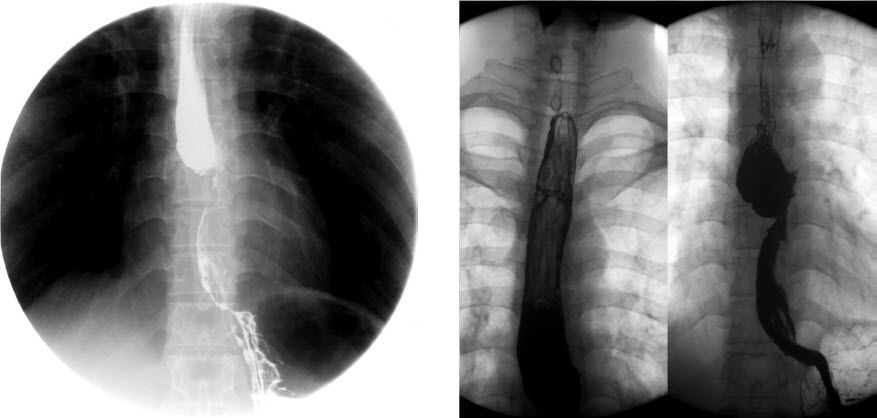
\includegraphics{./images/Image00247.jpg}
 \captionsetup{justification=centering}
 \caption{食管结核}
 \label{fig5-2-4}
  \end{figure} 

\textbf{【病史摘要】}
 男性,61岁。因突发大量呕血入院。近半年来感低热,胸骨后疼痛,有时为背痛,多呈持续性,吞咽时加重,体重减轻。

\textbf{【X线表现】}
 食管钡透示:食管中下段管腔狭窄明显,粘膜纹理粗乱不规则,管壁轮廓不规则呈锯齿状,可见小针刺状龛影,管壁僵硬不明显,仍有一定的扩张度,钡剂通过稍受阻。

\textbf{【X线诊断】}  食管中下段结核(溃疡型)。

\textbf{【评  述】}
 食管结核在临床极为少见。患者多以吞咽困难、吞咽痛或胸骨后疼痛为主诉就诊,缺乏典型的结核中毒症状。有的患者以呕血为首发症状,甚至表现为内科治疗无法控制的消化道大出血。食管结核的病理类型可分为3种:①溃疡型。②增殖型。③颗粒型。

食管结核的钡剂造影检查可以发现下列征象:①溃疡型几乎都发生在食管中段,主要表现为食管管腔溃疡,可见龛影,但也并非所有患者都能见到溃疡所形成的龛影这一征象。由于瘢痕收缩及周围组织粘连而使管腔轻度狭窄或正常,粘膜纹理粗乱不规则,管壁轮廓可不规则呈锯齿状,但管壁僵硬不明显,仍有一定的扩张度,钡剂可顺利通过。②增殖型多见于食管中段,其次为下段。X线检查多显示程度不等的管腔狭窄,为侧壁局限性充盈缺损,大小不一,管壁有一定弹性,钡剂通过缓慢,而无梗阻。在充盈缺损附近有软组织肿块影,为增厚的管壁或肿大的淋巴结,病变区域的粘膜纹理可以正常,或变形甚至完全消失。

食管结核主要应与食管癌进行鉴别,主要鉴别点为:①食管结核多发生于青壮年,年龄较轻,低于45岁,女性多见;而恶性肿瘤发病多在50岁以上,男性多见。②食管结核患者多有肺结核病史或结核接触史,胸部X线检查提示肺部有陈旧性结核或有活动性结核病灶。③食管结核临床症状轻,由于结核性食管狭窄引起的吞咽困难进展较缓慢,呈非进行性吞咽困难,与食物性状无关,病程常较短,抗结核药物治疗有效;食管恶性肿瘤引起的吞咽困难及胸痛呈进行性加重,常在短时期内(3个月至半年)出现重度吞咽困难,且一般情况恶化快。其病程较长,常伴消瘦症状。④食管结核皮肤结核菌素试验(PPD皮试)阳性、血清结核抗体阳性。⑤X线钡剂造影检查:食管结核食管腔有充盈缺损和溃疡,或粘膜呈虫蚀样改变,管壁稍僵硬,纵隔淋巴结结核压迫食管所致充盈缺损,多呈弧形,局部粘膜平整,附近有软组织肿块影或病变周围结核钙化影;而食管癌管壁不整、僵硬,粘膜明显破坏,充盈缺损明显且不规则。

\subsection{化学性食管炎}

\begin{figure}[!htbp]
 \centering
 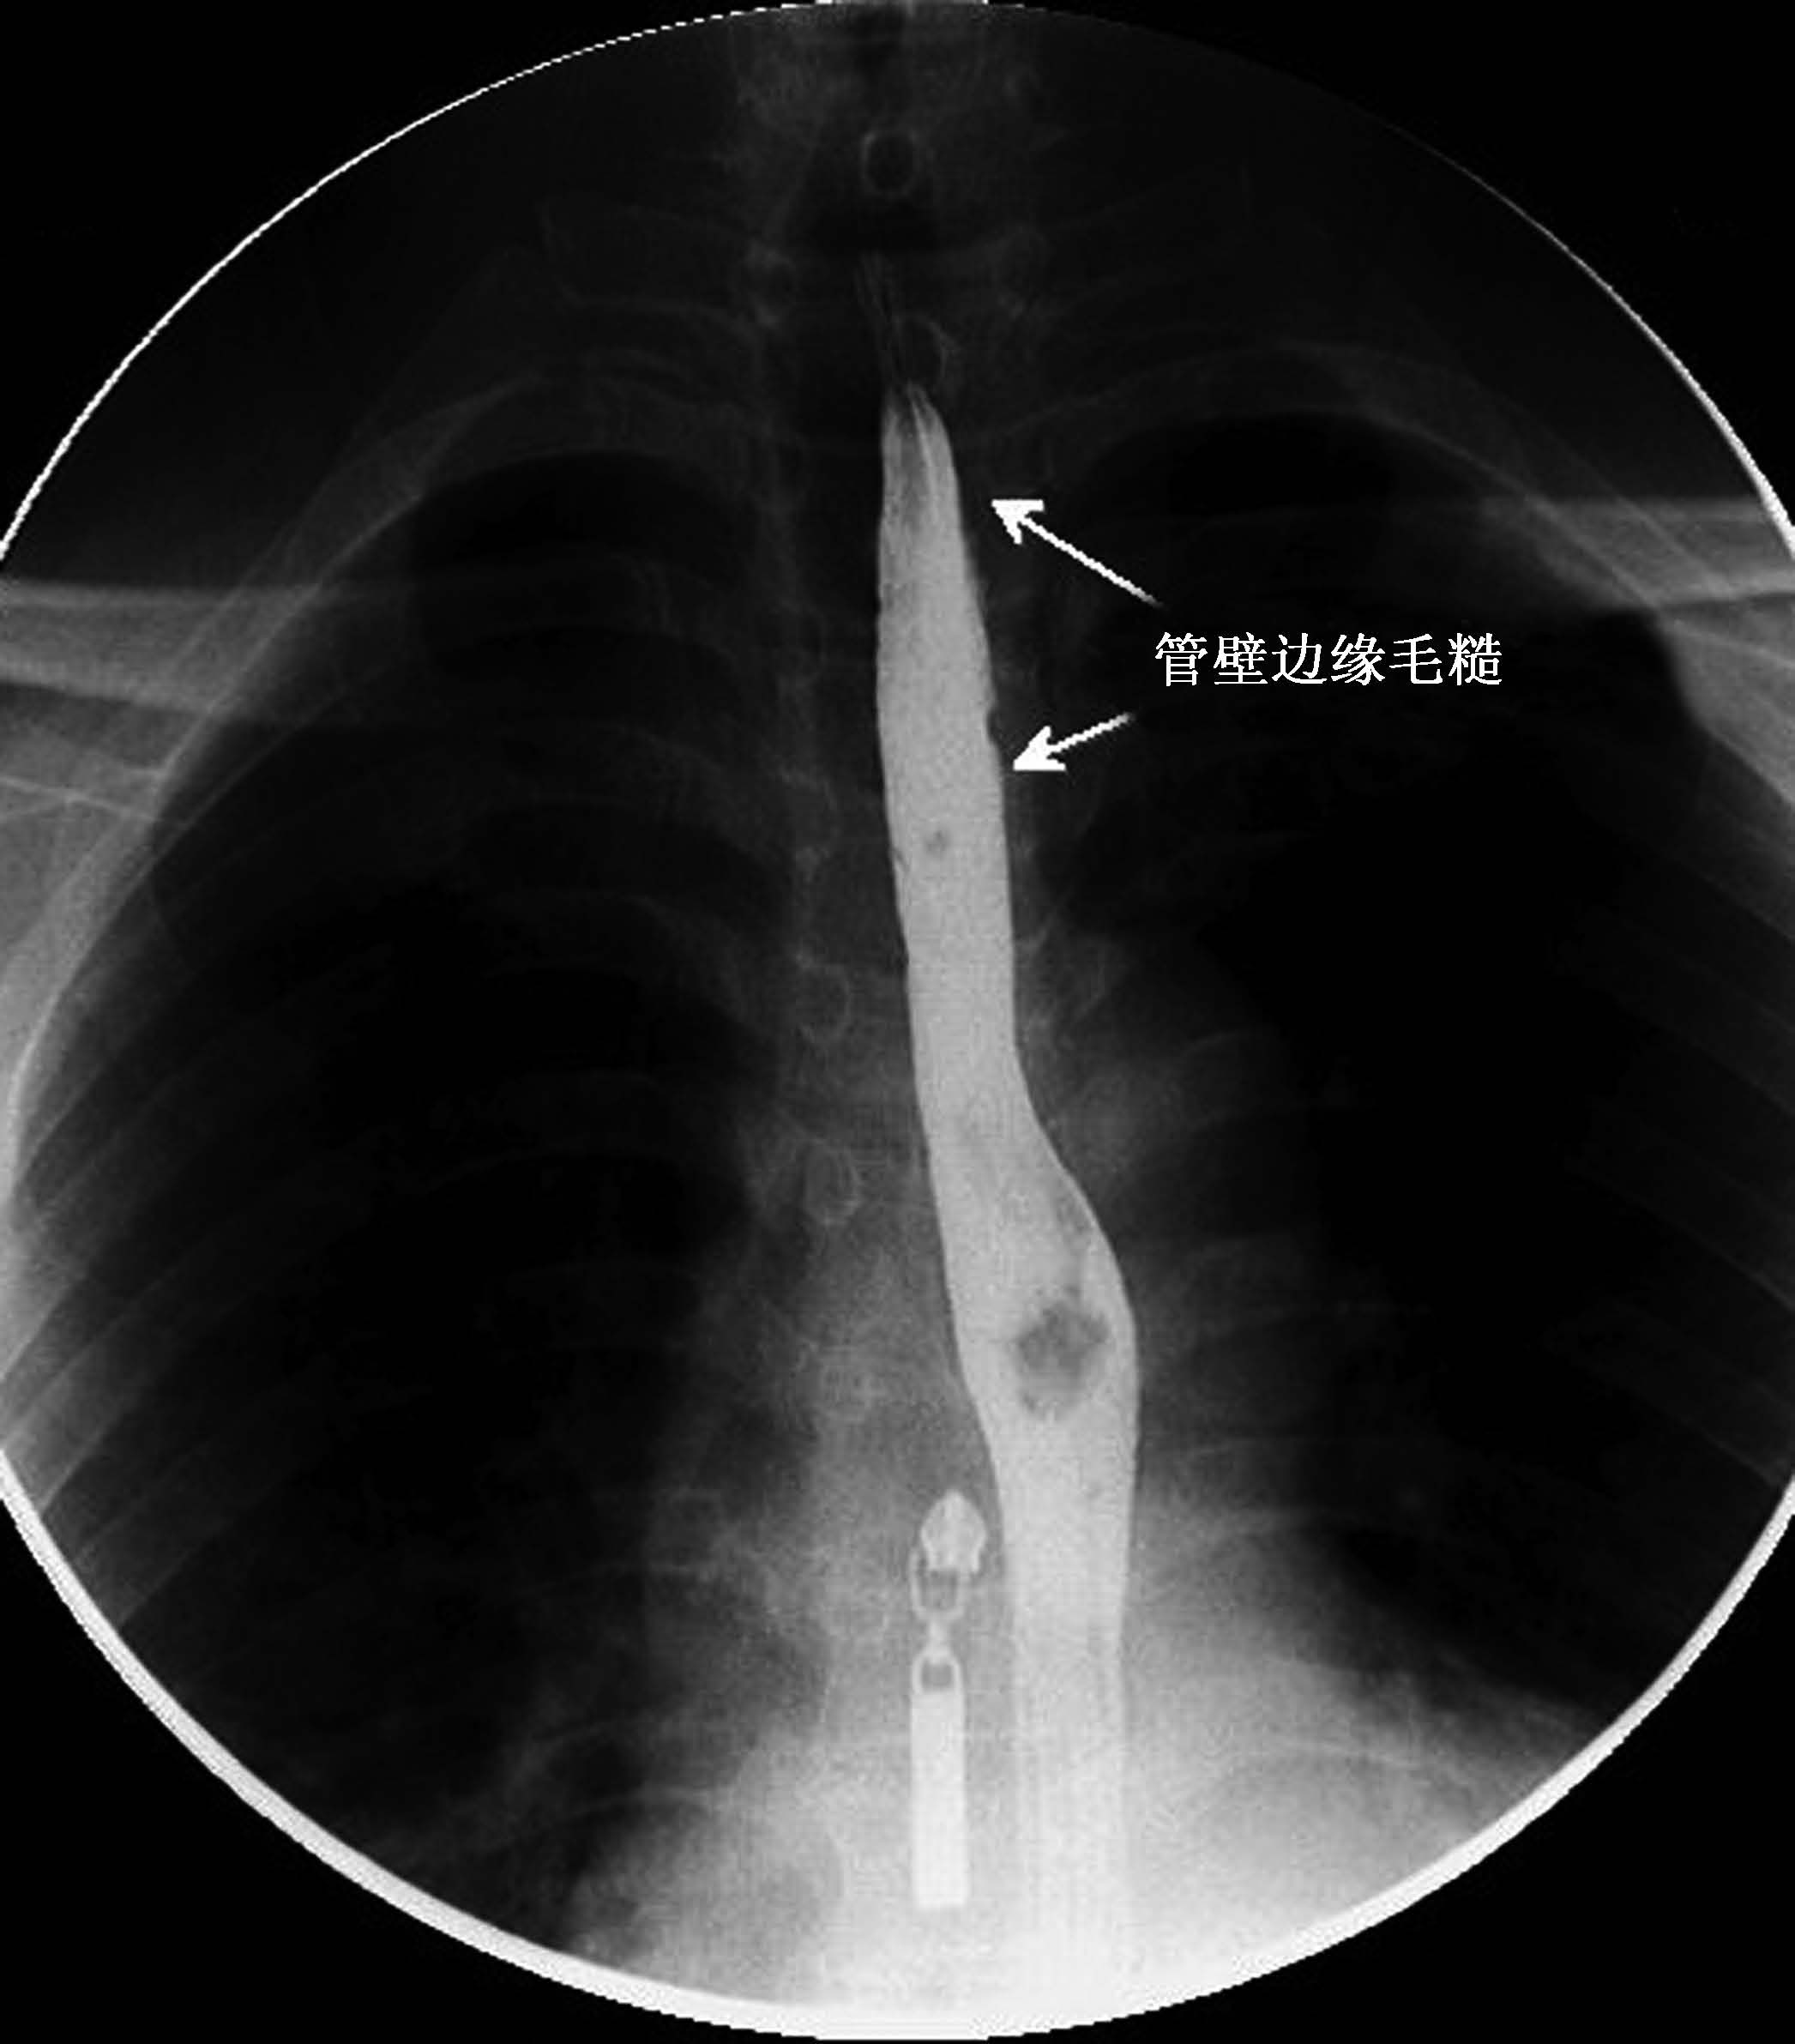
\includegraphics{./images/Image00248.jpg}
 \captionsetup{justification=centering}
 \caption{化学性食管炎}
 \label{fig5-2-5}
  \end{figure} 

\textbf{【病史摘要】}
 男性,20岁。因误服少量烧碱1小时入院,自述吞咽唾液时胸骨后疼痛伴吞咽困难。

\textbf{【X线表现】}
 食管钡透检查示食管上段管壁欠光整,边缘毛糙,食管蠕动较正常减弱。

\textbf{【X线诊断】}  化学性食管炎(烧碱)。

\textbf{【评  述】}
 化学腐蚀剂分为酸性和碱性两类。食管粘膜接触了化学腐蚀剂后,在病理上会产生一系列的变化:在短时间内(数小时至24小时内),食管壁会产生急性炎症反应,导致食管粘膜水肿、渗出、表面糜烂及激惹性的痉挛收缩而出现食管的早期明显狭窄或梗阻,如临床处理及时,在数天后水肿消退且同时伴随组织修补过程,进一步则进入瘢痕形成时期。食管受损的范围及程度与化学腐蚀剂的性质、浓度、剂量及服食速度有关。在急性期,主要表现为食管痉挛性收缩,管腔狭窄,病变以上管腔稍有扩大,病变部食管壁边缘不光滑,呈不规则或串珠状改变,粘膜像可显示粘膜增粗或消失;在恢复期,上述征象会有改善。但在病变后期,由于纤维组织增生及瘢痕形成,食管腔会显示连续性的进一步狭窄或间断性狭窄,边缘尚光整或稍不规则,粘膜消失,狭窄段以上食管扩张。

需要重点注意的是:一般需在临床紧急处理后,待病情稳定,再行食管钡餐检查。如怀疑有食管穿孔的可能性,则要求停用钡剂造影而改用碘油造影。

\subsection{食管静脉曲张}

\begin{figure}[!htbp]
 \centering
 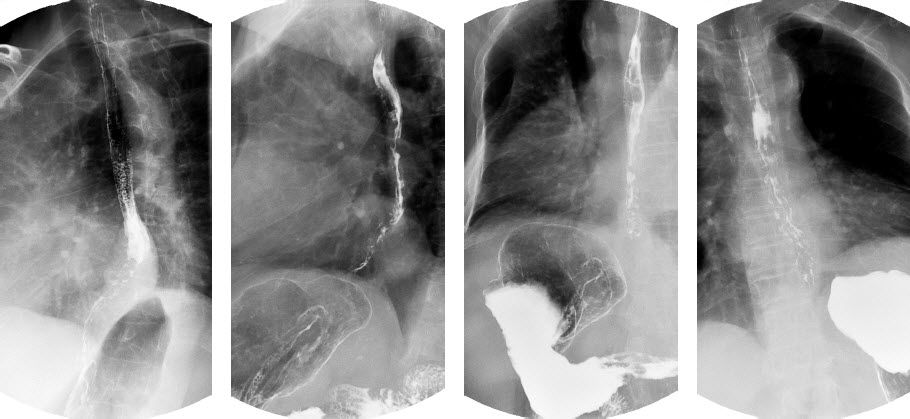
\includegraphics{./images/Image00249.jpg}
 \captionsetup{justification=centering}
 \caption{食管静脉曲张}
 \label{fig5-2-6}
  \end{figure} 

\textbf{【病史摘要】}
 男性,61岁。因突发呕血2小时入院,患肝硬化、脾大6年,腹水征阳性。

\textbf{【X线表现】}
 食管钡透示食管上、中、下段粘膜增粗、紊乱,其间可见串珠状或蚯蚓状充盈缺损,食管管壁边缘凹凸不平呈锯齿状,钡剂通过缓慢。

\textbf{【X线诊断】}  食管静脉曲张(重度)。

\textbf{【评  述】}
 轻度静脉曲张局限于食管下段,粘膜皱襞略增粗,管腔边缘可呈轻微的锯齿状,管壁张力无明显异常,此时如检查方法不当或观察不仔细可漏诊;中度静脉曲张,病变累及中段,粘膜皱襞明显增粗,呈串珠状或蚯蚓状,食管边缘呈明显的锯齿状,管壁张力欠佳,钡剂通过迟缓;重度静脉曲张,病变累及食管上段,甚至膈上全部食管,管腔明显扩张,正常粘膜被大小、形态不一的圆形、环形充盈缺损取代,形成链状,食管轮廓更加不整,但管壁柔软,钡剂通过更加迟缓。钡剂检查时,钡剂不宜过多,以避免对曲张的静脉形成物理性挤压作用;钡剂宜一次吞下,防止多次吞咽产生的气泡伪影,干扰诊断。

食管静脉曲张表现典型,如检查方法得当,诊断并不困难。需鉴别者有:①气泡影:随钡剂吞入的小气泡随检查时间推移而变动位置或消失,静脉曲张形态可变化但持续存在。②食管癌:虽然下段食管癌可呈息肉状改变,但其病变局限,边界分明,管壁僵直,粘膜中断、破坏,都具特征性,而与静脉曲张不同。

\subsection{食管功能性憩室}

\begin{figure}[!htbp]
 \centering
 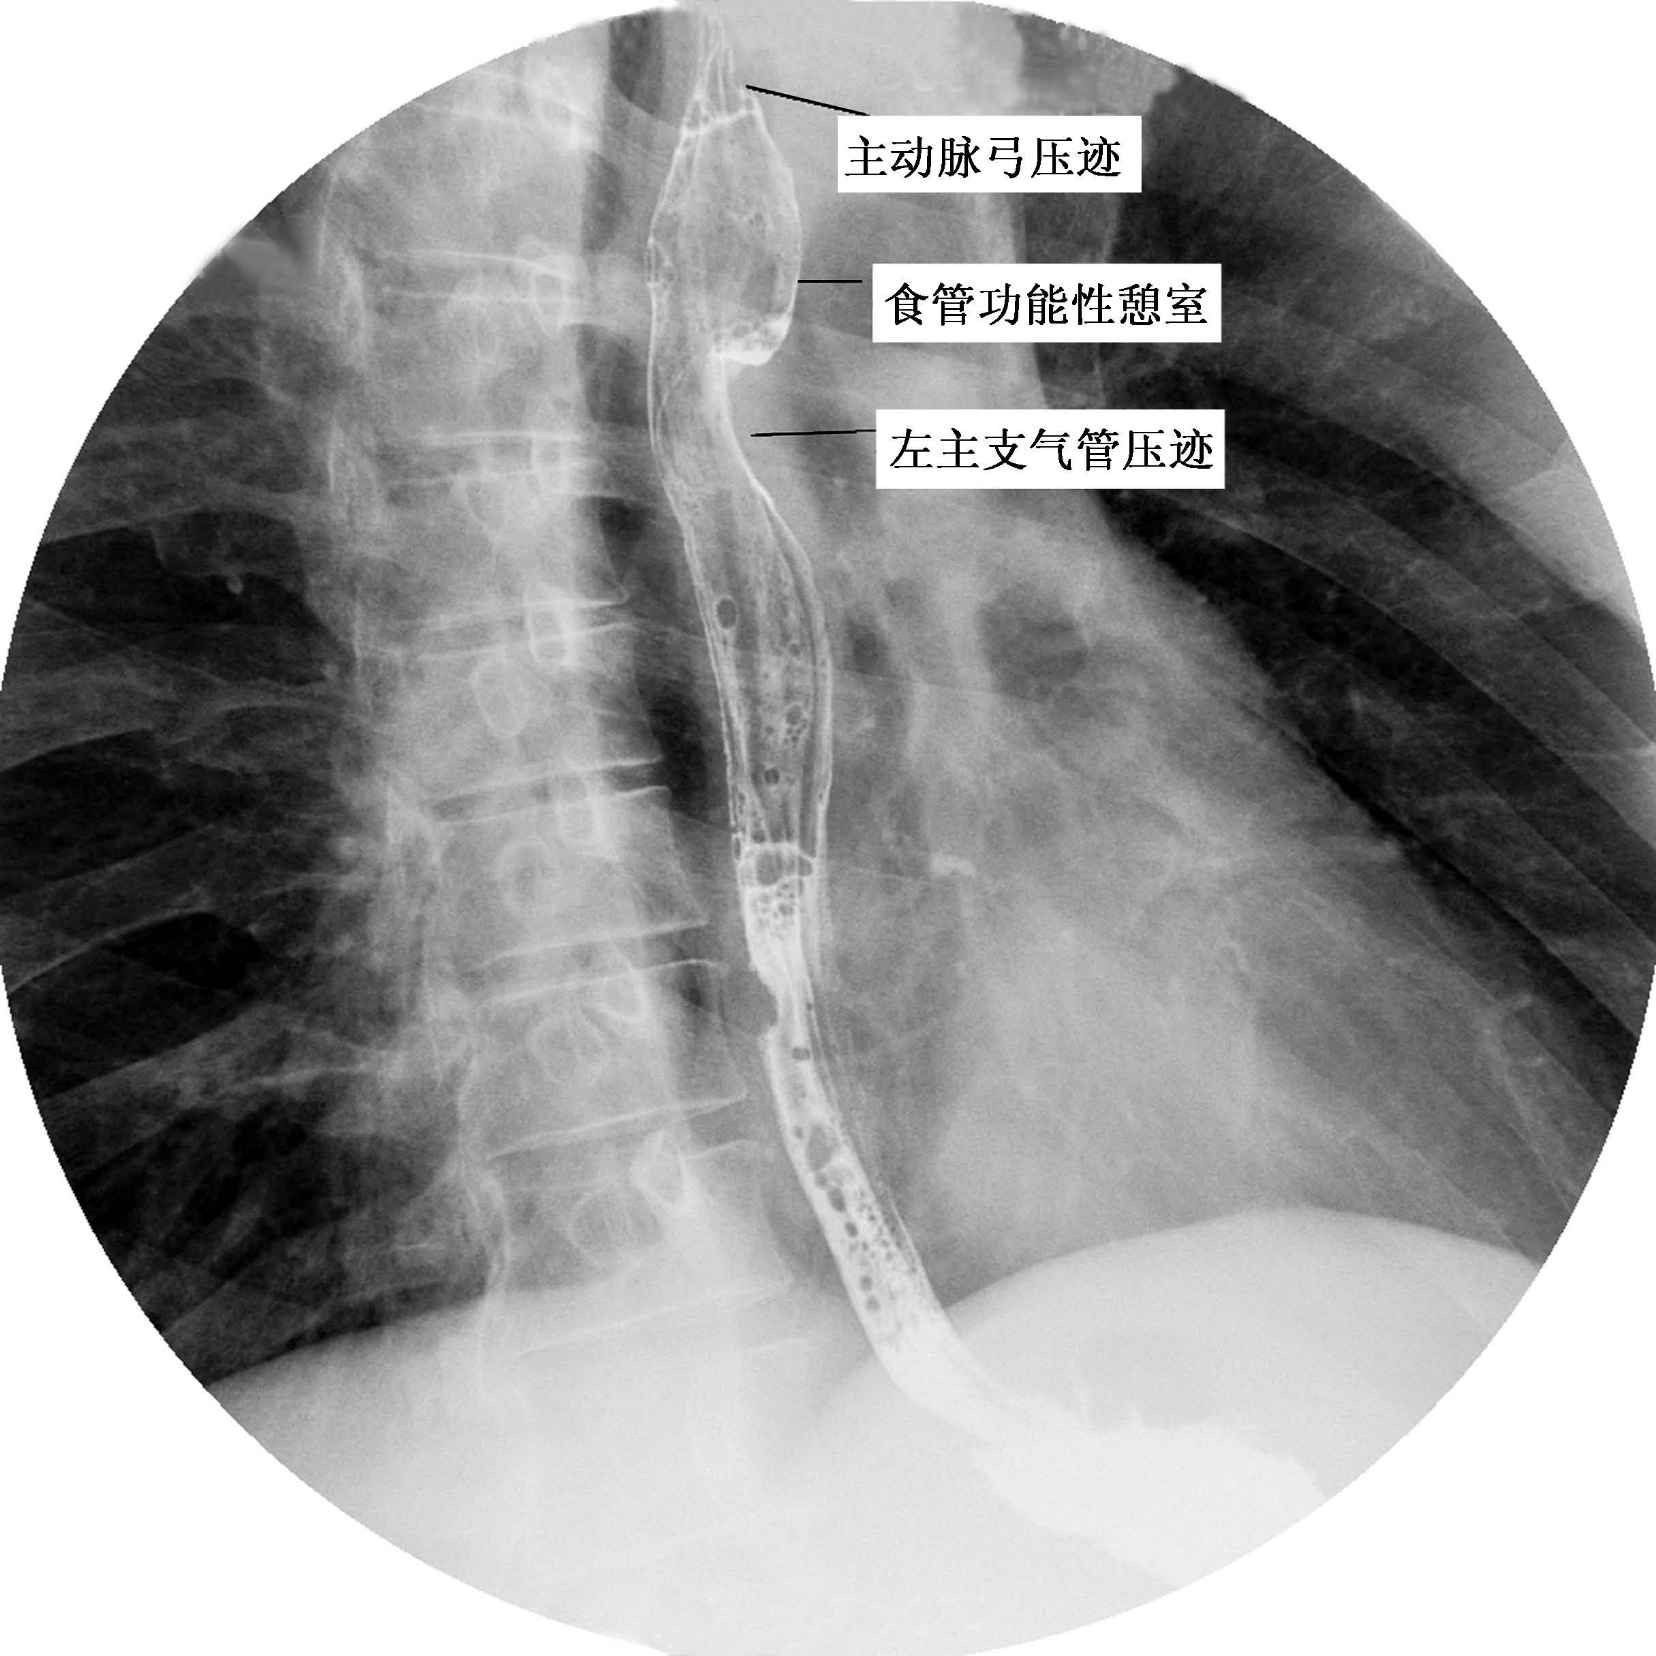
\includegraphics{./images/Image00250.jpg}
 \captionsetup{justification=centering}
 \caption{食管功能性憩室}
 \label{fig5-2-7}
  \end{figure} 

\textbf{【病史摘要】}  女性,30岁。因咽部不适,吞咽时有异物感。

\textbf{【X线表现】}
 食管钡透示食管上段主动脉弓下见囊袋状突起,食管壁柔软,钡剂下行顺畅。

\textbf{【X线诊断】}  食管功能性憩室。

\textbf{【评  述】}
 食管钡透时,可于主动脉弓压迹与左主支气管压迹之间,食管显示略膨出,注意不要误认为器质性憩室。

\subsection{食管憩室}

\begin{figure}[!htbp]
 \centering
 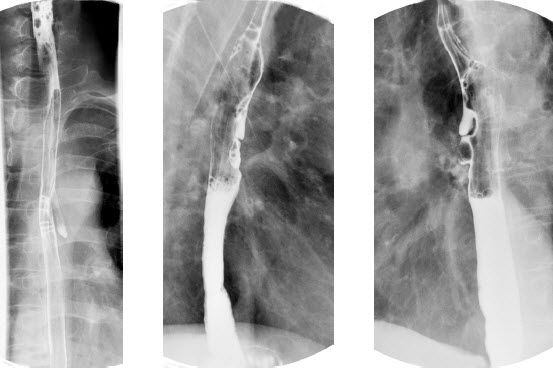
\includegraphics{./images/Image00251.jpg}
 \captionsetup{justification=centering}
 \caption{食管中段憩室}
 \label{fig5-2-8}
  \end{figure} 

\begin{figure}[!htbp]
 \centering
 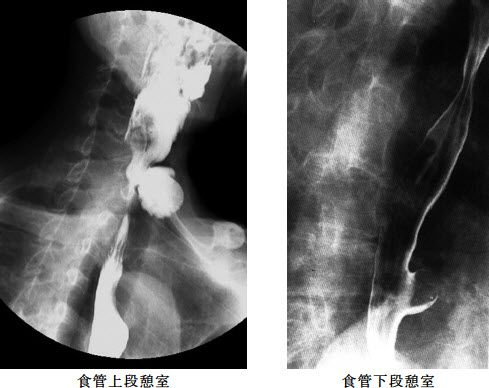
\includegraphics{./images/Image00252.jpg}
 \captionsetup{justification=centering}
 \caption{食管憩室}
 \label{fig5-2-9}
  \end{figure} 

\textbf{【病史摘要】}  女性,35岁。胸背部不适,吞咽时有哽噎感半年。

\textbf{【X线表现】}
 右前斜位及左前斜位示食管中段囊性突起影,内有钡剂充盈,体位改变后,钡剂部分流出。

\textbf{【X线诊断】}  食管中段憩室。

\textbf{【评  述】}
 食管憩室是食管管壁的囊袋状突出,根据发生的部位,分为咽食管憩室、食管中段憩室、膈上食管憩室。X线检查对憩室的诊断起决定作用。因绝大多数的憩室起自食管的前壁或右侧壁,因此,左前斜位或右前斜位显示较好;有时需做俯卧位,以便钡剂进入憩室。食管憩室吞钡检查表现为囊袋状突出影,边缘光滑整齐,口部较小或较宽,大小可变,有时可见粘膜皱襞伸入。咽食管憩室较大时第6颈椎前软组织增宽,其内可见液平;因常有滞留物(食物或粘液等),充钡时密度不均或呈分层状,大的憩室可压迫食管使其前移。食管中段憩室,多位于气管分叉部附近的前壁或侧前壁,憩室顶端可呈牵幕状,颈部较宽。憩室伴有炎症时,其边缘不规则,邻近食管可有痉挛。憩室穿孔时,可见造影剂流入纵隔或气管、支气管。需要重点注意的是:食管中段憩室应与主动脉和左主支气管压迹之间的食管膨出相鉴别;膈上食管大憩室应注意与食管裂孔疝鉴别,憩室囊袋状结构影与食管相连,而食管裂孔疝的膈上疝囊则通过裂孔与胃相连。

\subsection{食管颈椎增生压迹}

\begin{figure}[!htbp]
 \centering
 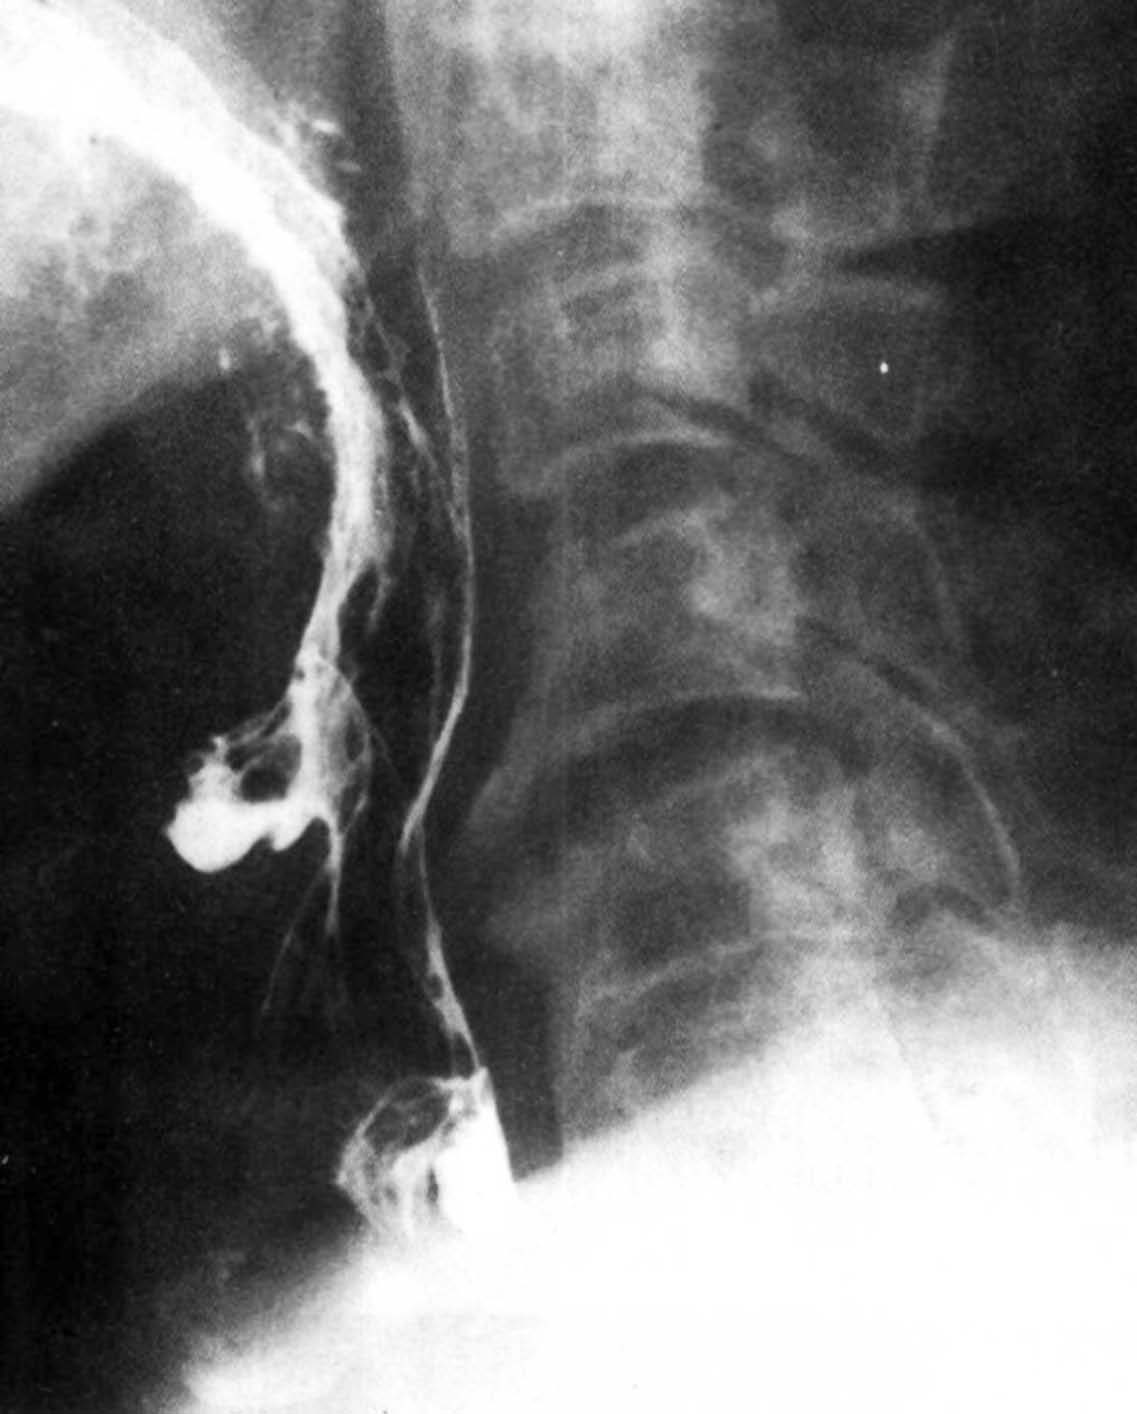
\includegraphics{./images/Image00253.jpg}
 \captionsetup{justification=centering}
 \caption{食管颈椎增生压迹}
 \label{fig5-2-10}
  \end{figure} 

\textbf{【病史摘要】}
 男性,69岁。颈椎部疼痛,伴左侧前臂麻木,伴有吞咽时哽噎感。

\textbf{【X线表现】}
 食管上段钡透侧位片示:食管上段平4、5椎体水平后缘见弧形压迹,食管壁柔软,颈椎生理弧度僵直,第4、5颈椎体前缘见唇样骨赘形成。

\textbf{【X线诊断】}  食管颈椎增生压迹。

\textbf{【评  述】}
 食管为后纵隔的肌性器官,两端固定,中间可以移动。食管外压性改变可以是由于脊柱椎体骨质过度增生对食管后方产生局部压迫。临床上多有原发疾病的症状,伴有不同程度的吞咽困难或吞咽受阻感。

\subsection{贲门失迟缓症}

\begin{figure}[!htbp]
 \centering
 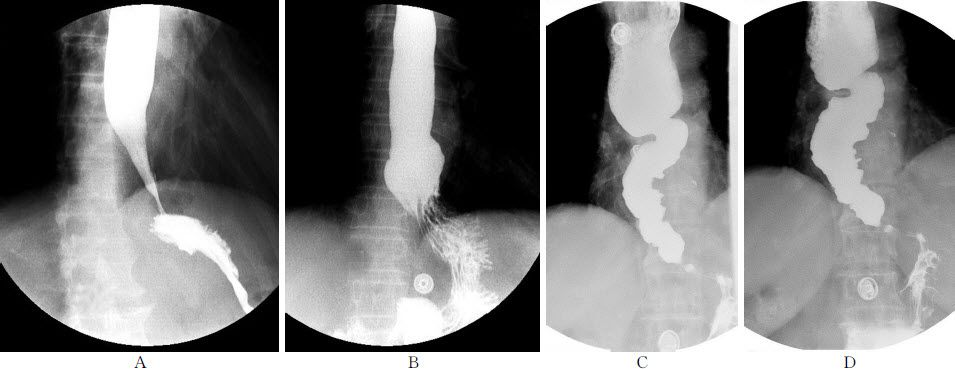
\includegraphics{./images/Image00254.jpg}
 \captionsetup{justification=centering}
 \caption{贲门失迟缓症}
 \label{fig5-2-11}
  \end{figure} 

\textbf{【病史摘要】}
 女性,45岁。间歇性胸骨后疼痛,吞咽困难2~3年,近年来自觉胸闷心慌,吞咽困难呈持续性,有时伴有呕吐。

\textbf{【X线表现】}
 食管显著扩张,管径5cm左右,下段扩张,呈萝卜根状,腔内多量钡剂潴留,中下段食管蠕动消失。狭窄段食管管壁光滑,柔软(图A、B)。

\textbf{【X线诊断】}  贲门失迟缓症(早期)。

\textbf{【评  述】}
 本病病因不明,一般认为是由于迷走神经的退行性变所致。临床一般见于20~40岁,女性较多。病程长,可数月至数年,常见症状为吞咽困难,胸骨后有阻塞感,以进食固体性食物时明显,症状时轻时重,与精神因素有一定关系。进食较快或梗阻严重时可出现呕吐。严重的食管失迟缓症,胸部X线片可因高度扩张的食管,使纵隔增宽,其内常有液平,而不致误为纵隔肿瘤。一般需钡餐造影确诊。早期,食管轻度扩张,以下半部明显。食管正常蠕动减弱或消失,代之以紊乱的环肌收缩,食管下端呈漏斗状进入膈下,狭窄段为1~4cm,边缘光滑整齐。呼气时狭窄段管腔可略增宽,吸气时变窄,因此,钡剂可随呼吸断续通过。狭窄段的粘膜细而平行,有利于与浸润型食管癌鉴别。晚期,食管显著扩张、延长、迂曲,食管的不规则收缩减弱或消失,或在服钡的瞬间看到几个蠕动波。第一口钡剂有时可少量通过狭窄段,之后连续服钡,需达一定量,常到主动脉弓水平或更高,借助钡剂的重力,才可经狭窄段喷射进入胃内。食管下段呈S形弯曲,下端呈鸟嘴状,边缘光滑、对称。深呼吸时膈肌裂孔迟缓,狭窄段可略变宽(图C、D)。这种随膈肌裂孔张缩而出现的变化,说明管壁柔软,有助于与食管癌鉴别。

\subsection{食管裂孔疝}

\begin{figure}[!htbp]
 \centering
 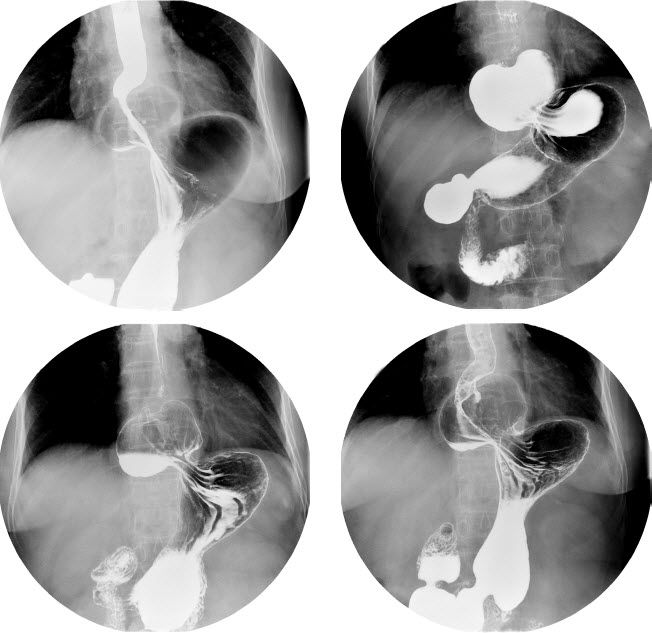
\includegraphics{./images/Image00255.jpg}
 \captionsetup{justification=centering}
 \caption{食管裂孔疝}
 \label{fig5-2-12}
  \end{figure} 

\textbf{【病史摘要】}
 女性,35岁。胸骨后不适、烧灼、疼痛2年余,饱食后平卧位症状加重,疼痛向肩部放射。

\textbf{【X线表现】}
 左侧膈上见大小约3.5cm×4.0cm的疝囊影,内见粗大弯曲粘膜皱襞,下方见较宽粘膜皱襞通过裂孔与胃相连,贲门位于膈上疝囊内。

\textbf{【X线诊断】}  食管裂孔疝。

\textbf{【评  述】}
 腹腔内脏器移位于胸腔,称为膈疝。腹腔内脏器经食管裂孔疝入胸腔者,称食管裂孔疝,约占膈疝的70%。一般将食管裂孔疝分为四型:①可复型食管裂孔疝。②牵引型食管裂孔疝。③食管旁食管裂孔疝。④先天性短食管型裂孔疝。X线检查为食管裂孔疝的可靠的检查方法。

食管裂孔疝常用检查方法是:①仰卧头低足高位大量服钡使胃过度充盈,之后从右前斜位转至左前斜位,或患者仰卧直腿抬高同时腹部加压。②卧位Valsalva呼吸实验。③胃充满后侧立位弯腰,有利于疝囊的显示。

食管裂孔疝的X线表现有:①膈上疝囊:为疝入胸腔的小部分胃构成,除食管旁型裂孔疝外,皆包括胃食管前庭部。疝囊呈圆柱状或漏斗状,疝囊上方可见下食管括约肌形成的收缩区,称A环。②食管胃环:为食管粘膜与胃粘膜交界部,正常位于膈下,不能显示,裂孔疝时,疝入胸腔,变为疝囊两侧对称性、局限性切迹,称B环。③膈上出现胃粘膜:表现为粗大迂曲的皱襞。④胃小区:个别患者双重造影时,裂孔上出现胃小区。⑤鸟嘴征:仰卧位时,钡剂使贲门轻度张开,形似鸟嘴状,常与其他裂孔疝之X线征象并存。⑥孔征:膈上胃囊充气时,轴位投影于胃底,其形态似孔,称孔征。⑦食管旁型食管裂孔疝:贲门仍位于膈下,疝囊在食管左前方,较大时可压迫食管。根据以上表现,裂孔疝诊断不难。在鉴别诊断方面,应注意不可将食管膈壶腹误为裂孔疝,前者为生理性表现,位于膈上4~5cm一段食管,扩大呈椭圆形,粘膜为纵行纤细的食管粘膜,无下食管括约肌收缩环及疝囊表现。膈上憩室,扩大的囊腔与食管有窄颈相连,其下有一段正常食管通过食管裂孔与贲门相连,胃底正常。

\subsection{食管平滑肌瘤}

\begin{figure}[!htbp]
 \centering
 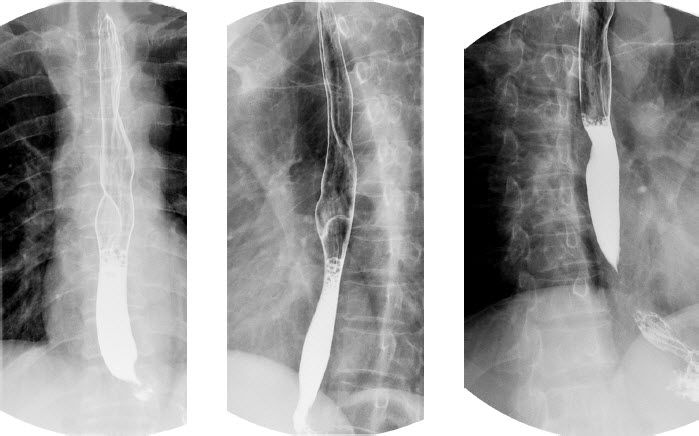
\includegraphics{./images/Image00256.jpg}
 \captionsetup{justification=centering}
 \caption{食管平滑肌瘤}
 \label{fig5-2-13}
  \end{figure} 

\textbf{【病史摘要】}
 女性,45岁。近2年来进食时有哽噎感,无异物感及疼痛,既往体健,无消瘦。

\textbf{【X线表现】}
 食管钡透检查,示食管中下段椭圆形充盈缺损,见环形征,边缘光滑,食管粘膜未见明显中断、破坏,管腔无明显狭窄,管壁柔软无僵硬。

\textbf{【X线诊断】}  食管中下段平滑肌瘤。

\textbf{【评  述】}
 食管平滑肌瘤是最常见的食管良性肿瘤,占食管良性肿瘤的2/3。食管平滑肌瘤起自平滑肌层或粘膜肌层,位于壁内粘膜下,呈膨胀性生长。平滑肌瘤可发生于食管的各段,以中下段多见。钡餐检查最常见的征象为充盈缺损,呈圆形、椭圆形,边界清楚,较多钡剂通过后,肿瘤周围仍有钡剂存留,形成所谓环形征;肿瘤表面粘膜可变宽或展平,少数病例可见溃疡龛影。钡剂通过肿瘤部位时,在正位,钡剂自肿瘤两侧分流,管腔可变宽;切线位时,钡剂偏流而过。食管平滑肌瘤和壁内其他良性肿瘤的X线征象相似,难以鉴别。恶性肿瘤中食管平滑肌肉瘤罕见,可分息肉型及浸润型,前者多表现为不规则的分叶状或表面有大小不等的息肉状充盈缺损,易发生溃疡;后者与食管癌相似。食管平滑肌瘤则极少发生溃疡,其典型表现为规则的圆形或类圆形充盈缺损。平滑肌瘤与食管癌的鉴别,主要是癌瘤不规则,粘膜破坏,及浸润性生长而致管腔狭窄、僵硬等。

\subsection{食管癌(早期)}

\begin{figure}[!htbp]
 \centering
 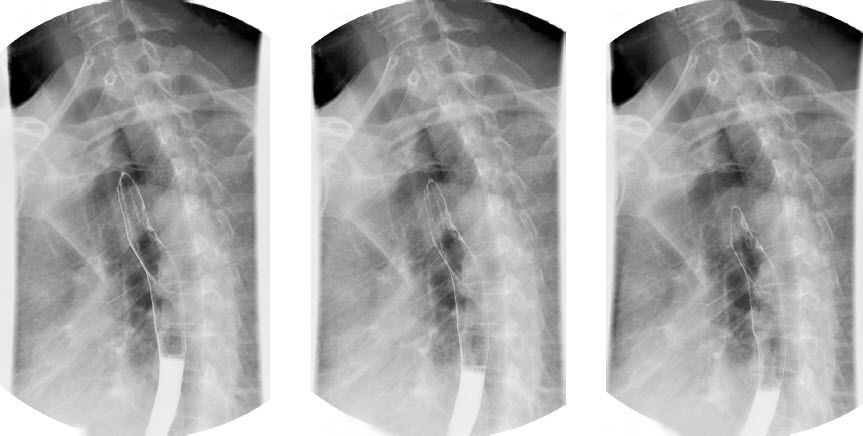
\includegraphics{./images/Image00257.jpg}
 \captionsetup{justification=centering}
 \caption{食管癌(早期)}
 \label{fig5-2-14}
  \end{figure} 

\textbf{【病史摘要】}  男性,65岁。咽部不适伴胸骨后轻微疼痛6个月余。

\textbf{【X线表现】}
 食管钡透示:食管上段平第6、7胸椎水平局限性粘膜皱襞扭曲、中断。食管管壁边缘毛糙,呈轻度缩窄,食管蠕动较差。

\textbf{【X线诊断】}  食管上段早期癌。

\textbf{【评  述】}
 本例经手术证实为早期食管癌。早期食管癌病变表浅,X线改变比较轻微,由于造影检查时食管粘膜皱襞显示不清,诊断往往困难。所以早期食管癌的X线检查,应重点注意食管的蠕动、管壁的扩张情况,并多轴位的双重造影像及粘膜像结合诊断。早期食管癌的X线表现主要为:①食管粘膜皱襞的改变:粘膜皱襞增粗、迂曲,有1~2条粘膜皱襞中断,边缘毛糙。②形成小溃疡:在紊乱粗糙的粘膜面上出现小溃疡,可单发或多发,大小不等,一般在0.2~0.4cm,局部管壁轻度痉挛。③局限性小充盈缺损:直径多在0.5cm左右,最大不超过2cm,边缘毛糙,局部粘膜紊乱,少数病例在充盈缺损的病灶中有米粒样龛影。④管壁局限性僵硬:少数病例出现局限性舒展度减低,偏侧性管壁僵直。钡剂在此处通过减慢,呈滞留现象,或出现痉挛性收缩波。在粘膜像阴性情况下,这些征象可作为早期食管癌的定位征象。

\subsection{进展期食管癌(浸润型)}

\begin{figure}[!htbp]
 \centering
 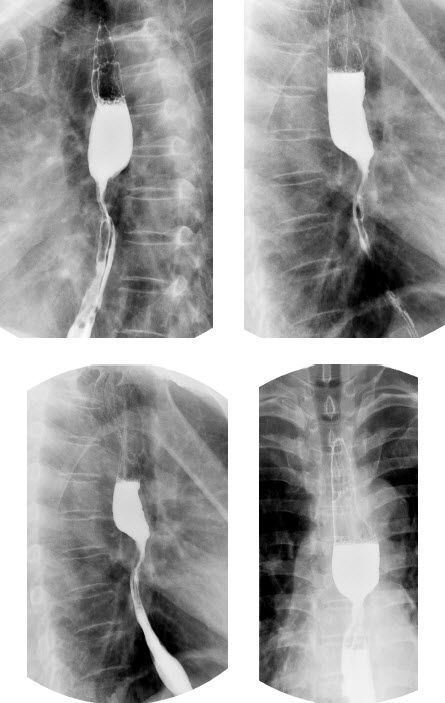
\includegraphics{./images/Image00258.jpg}
 \captionsetup{justification=centering}
 \caption{进展期食管癌(浸润型)}
 \label{fig5-2-15}
  \end{figure} 

\textbf{【病史摘要】}
 男性,56岁。进行性吞咽困难5个月余,近1个月来感胸骨后疼痛,只能进流质,并有呕吐症状。

\textbf{【X线表现】}
 食管钡透示:食管中下段管腔环形狭窄,钡剂下行受阻,狭窄段呈漏斗状,管壁僵硬,蠕动消失,狭窄段以上食管扩张明显。

\textbf{【X线诊断】}  进展期食管癌(浸润型)。

\subsection{进展期食管癌(溃疡型)}

\begin{figure}[!htbp]
 \centering
 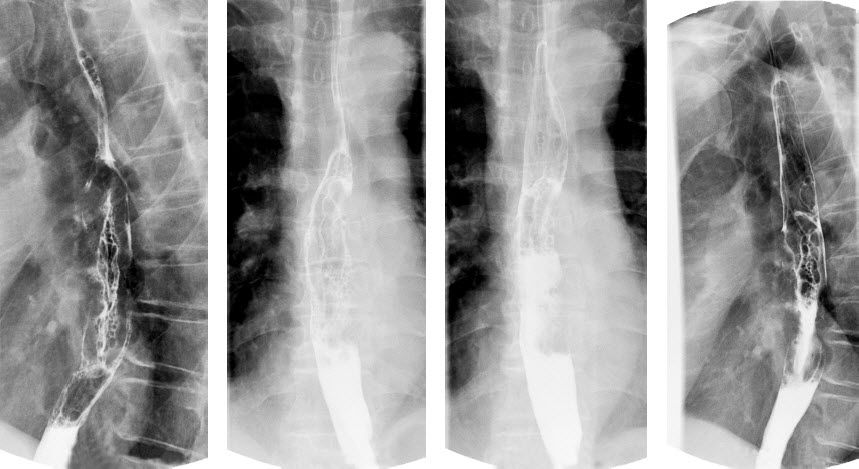
\includegraphics{./images/Image00259.jpg}
 \captionsetup{justification=centering}
 \caption{进展期食管癌(溃疡型)}
 \label{fig5-2-16}
  \end{figure} 

\textbf{【病史摘要】}
 女性,48岁。进行性吞咽困难3个月,近期进食流质时出现哽噎,消瘦。

\textbf{【X线表现】}
 食管钡透示:食管中下段管腔局限性狭窄,粘膜皱襞中断破坏,并见一较大龛影,与食管纵轴一致,切线位位于食管轮廓之内。

\textbf{【X线诊断】}  进展期食管癌(溃疡型)。

\subsection{进展期食管癌(增生型)}

\begin{figure}[!htbp]
 \centering
 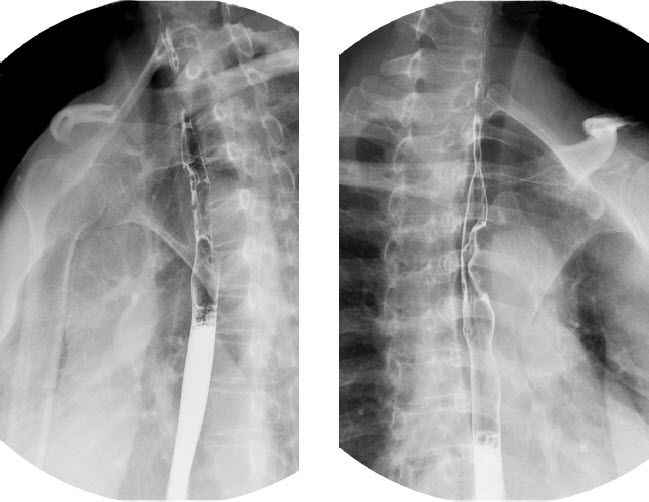
\includegraphics{./images/Image00260.jpg}
 \captionsetup{justification=centering}
 \caption{进展期食管癌(增生型)}
 \label{fig5-2-17}
  \end{figure} 

\textbf{【病史摘要】}
 男性,45岁。进行性吞咽困难3个月余,近期进食固体类食物时下咽困难,流质尚可,既往体健。

\textbf{【X线表现】}
 食管钡透示:食管中上段管腔内见不规则充盈缺损,管腔呈偏心性狭窄,充盈缺损基底部管壁僵硬,蠕动消失。

\textbf{【X线诊断】}  进展期食管癌(增生型)。

\textbf{【评  述】}
 本病一般分为三型:浸润型、溃疡型、增生型。进展期食管癌侵及肌层后,进展加快,X线征象也日益显著,主要表现为:①粘膜皱襞增粗、紊乱、中断、破坏,代之以肿瘤形成的不规则影。②病变区管腔不规则、偏心性狭窄,管壁僵硬,伴有梗阻征,其近端食管扩张。③腔内不规则的充盈缺损,其表面常有破坏形成的龛影。④不规则的龛影,位于食管轮廓之内。上述征象常混合存在。

食管癌的类型不同,X线表现也各具特征:①浸润型:管腔呈环形狭窄,范围局限,一般为3~5cm,严重时呈漏斗状,管壁僵硬,边缘多较光滑,上段食管扩张明显。②增生型:以腔内不规则的充盈缺损及管腔偏心性不规则的狭窄为特征,充盈缺损表面常有不规则的溃疡,为肿瘤坏死所致。③溃疡型:以边界清楚、形态不规则的龛影为特征。龛影多较长,与食管纵轴一致,在切线位多在食管轮廓线内,较深时可超出食管轮廓以外。溃疡周围隆起明显者,可见环堤征。增生型食管癌需注意与良性肿瘤中最多见的平滑肌瘤相鉴别,后者切线位也可表现为管腔内圆形或椭圆形充盈缺损,致食管管腔狭窄,但其边缘一般光滑、肿瘤区粘膜皱襞可消失而周围粘膜皱襞正常,管壁柔软,正位可显示钡剂环绕形成的环形征,管腔可变宽,管腔外可见软组织肿块影是其特征。增生型食管癌,特别是较大者与恶性癌肉瘤X线区分有一定难度,可以作为参考的是癌肉瘤虽然肿瘤较大,与食管癌相比较,患者临床梗阻症状一般较轻,癌肉瘤多发生在食管中下段,管腔外往往可显示有软组织块影,而食管癌最常见发生在食管中上段,管腔外较少形成软组织肿块影,两者表现不同,有时也需结合内镜病理活检方可鉴别。

\subsection{食管平滑肌肉瘤}

\begin{figure}[!htbp]
 \centering
 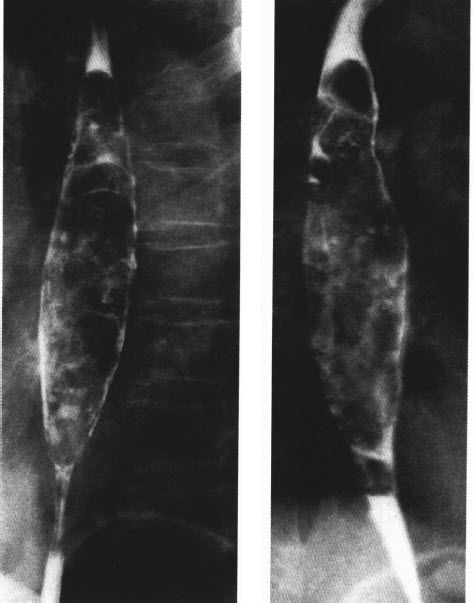
\includegraphics{./images/Image00261.jpg}
 \captionsetup{justification=centering}
 \caption{食管平滑肌肉瘤}
 \label{fig5-2-18}
  \end{figure} 

\textbf{【病史摘要】}
 男性,62岁。自述吞咽困难3个月,胸骨后感疼痛,既往体健。

\textbf{【X线表现】}
 食管钡透示:食管中下段管腔呈梭形扩张,内见多枚大小不等类圆形充盈缺损,食管壁尚光滑,食管粘膜皱襞消失。

\textbf{【X线诊断】}  食管平滑肌肉瘤。

\textbf{【评  述】}
 本病少见。好发于食管中下段,多呈息肉状突入管腔,少数为浸润性生长,肿瘤常限于粘膜或粘膜下层,个别为环形浸润,很少转移,预后较好。临床表现不具特征性,常因吞咽困难就诊。X线表现典型者为食管中下段腔内息肉状充盈缺损,基底小,可有蒂,局部管腔扩张。少数不典型者,如呈环形浸润性生长者与增生型食管癌难于诊断,需结合内镜病理活检方可鉴别。

\section{胃部病变}

\subsection{胃憩室}

\begin{figure}[!htbp]
 \centering
 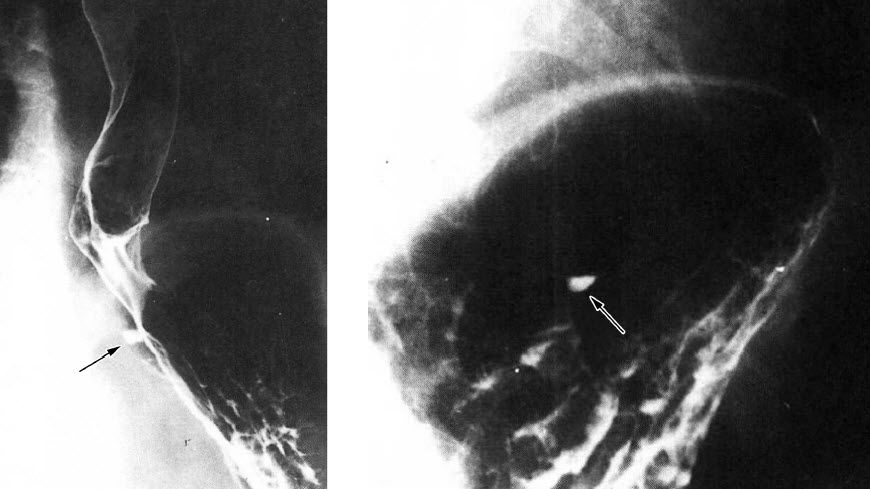
\includegraphics{./images/Image00262.jpg}
 \captionsetup{justification=centering}
 \caption{胃底憩室}
 \label{fig5-3-1}
  \end{figure} 

\textbf{【病史摘要】}
 女性,31岁。上腹部不适1周,无嗳气、反酸,无腹胀。体格检查:上腹部无明显压痛,肝、脾未及,心肺阴性。

\textbf{【X线表现】}
 胃钡透示:胃底部见囊袋状突起,边缘光滑整齐,内见钡剂残留,颈部狭窄,胃底粘膜伸入囊袋。

\textbf{【X线诊断】}  胃底憩室。

\textbf{【评  述】}
 本病一般为单发,80%位于贲门下方小弯侧的后壁,其次为幽门前区。憩室呈圆形或囊袋状,颈部狭窄、光滑。缺乏肌层者无收缩力,常因食物残留而致憩室炎。胃周粘连牵拉所致者,口部较宽,很少有食物残留。憩室有完整的粘膜层。胃憩室多无症状。伴发憩室炎时,可有腹痛、腹胀、恶心、呕吐及出血表现。X线表现主要有:①憩室外形光滑,如囊袋状影突出于胃腔之外,但基底部与胃相连,颈部略细。②粘膜像可见胃粘膜皱襞自颈部与憩室相连。③如合并憩室炎,其外形变得不规则,并可见局部胃壁痉挛变形等改变。根据憩室上述X线表现特点,尤其要注意粘膜皱襞形态,易与胃穿透性溃疡鉴别。憩室呈光滑的囊袋状,有正常的粘膜伸入其内,而没有粘膜皱襞纠集等表现;穿透性溃疡无粘膜皱襞伸入其中是与胃憩室区别之要点。

\subsection{胃底静脉曲张}

\begin{figure}[!htbp]
 \centering
 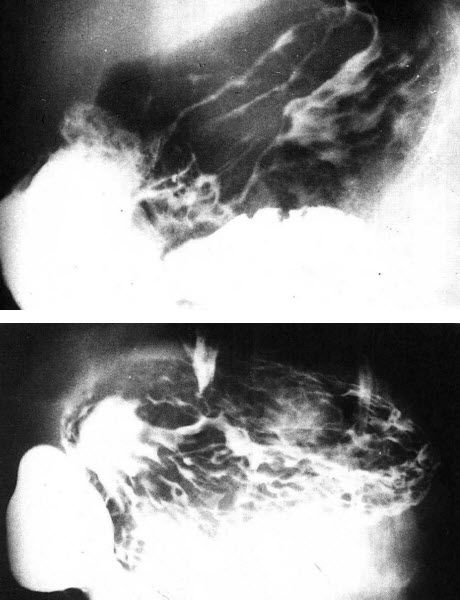
\includegraphics{./images/Image00263.jpg}
 \captionsetup{justification=centering}
 \caption{胃底静脉曲张}
 \label{fig5-3-2}
  \end{figure} 

\textbf{【病史摘要】}
 男性,61岁。患肝硬化多年,突发呕血1天伴黑便。体格检查:肝、脾大,腹水征阳性,腹壁静脉曲张,功能异常。

\textbf{【X线表现】}
 胃钡透示:胃底粘膜皱襞增宽迂曲,呈蚯蚓状,边缘光滑,未见明显中断破坏。

\textbf{【X线诊断】}  胃底静脉曲张。

\textbf{【评  述】}
 本病患者除具有门脉高压症的表现外(如肝脾肿大、脾功能亢进、肝功能异常、腹水、腹壁静脉曲张等),主要表现为呕血及黑便。X线检查具有安全、简便、准确的特点,易为患者接受。胃底静脉曲张常与食管静脉曲张并存,但也可单独存在,双对比造影可提高其显示率。胃底静脉曲张一般可分为两型:①泡沫型:胃贲门区及胃底粘膜呈葡萄状或息肉状透亮区,直径1~2cm,周围见薄层钡剂环绕,形如泡沫状。②肿块型:胃贲门区及胃底呈分叶状或团块状边缘光滑的充盈缺损。除上述表现外,胃底静脉曲张时,胃底与膈肌间距可增大,胃贲门角增大。因多伴有脾肿大,可造成胃的压迫性移位。胃底静脉曲张主要应与胃癌鉴别,静脉曲张形成的肿块影边缘光滑锐利,胃壁柔软(可借助气钡双重造影、呼吸动作或心脏搏动观察),贲门及腹段食管不被侵犯,结合临床病史,可以鉴别,个别病例可借助内镜检查或选择性血管造影帮助鉴别。

\subsection{胃内异物}

\begin{figure}[!htbp]
 \centering
 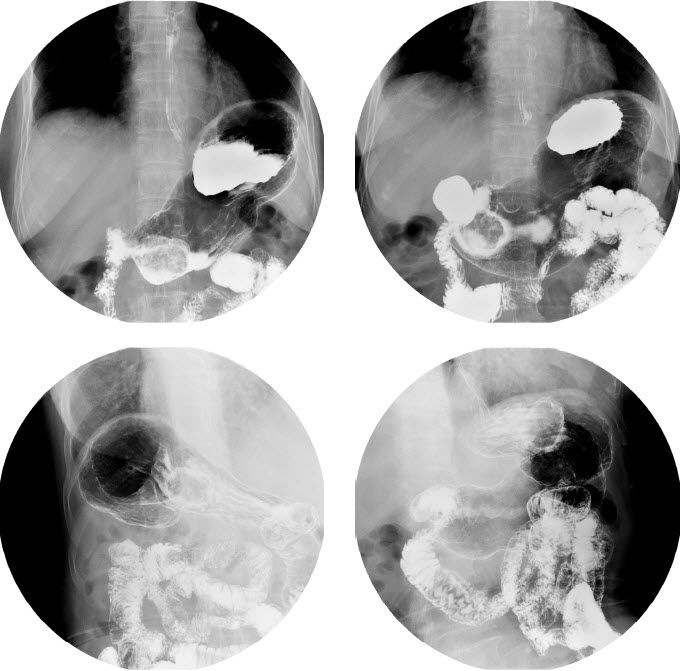
\includegraphics{./images/Image00264.jpg}
 \captionsetup{justification=centering}
 \caption{胃内异物(胃柿石)}
 \label{fig5-3-3}
  \end{figure} 

\textbf{【病史摘要】}
 女性,35岁。上腹部不适伴疼痛2个月余,可自行缓解,近期有大量进食柿子史。

\textbf{【X线表现】}
 胃钡透示:胃窦部见类圆形充盈缺损影,大小4cm×3.5cm左右,边缘稍毛糙,表面见凹凸不平的不规则钡斑,体位改变后,充盈缺损位置改变。

\textbf{【X线诊断】}  胃内异物(胃柿石)。

\textbf{【评  述】}
 柿子、豆类、毛发、绒线及粘液性物质进入胃内,因机械作用而相互缠绕成团,形成胃石。在产柿地区,胃柿石是最常见的胃石。因进食大量不成熟柿子后,与胃酸起作用,凝结成块,而成胃石。X线表现胃内可见类圆形充盈缺损影,体积可以很大,也可分成数块,表面凹凸不平,呈现不规则的钡斑。充盈缺损可在胃内移动,压迫或变动体位,其位置有变化。此外,周围胃壁柔软,蠕动正常,这些特点可与胃肿瘤相鉴别。特别注意的是要结合临床病史做出最后诊断。

\subsection{幽门肌肥厚症}

\begin{figure}[!htbp]
 \centering
 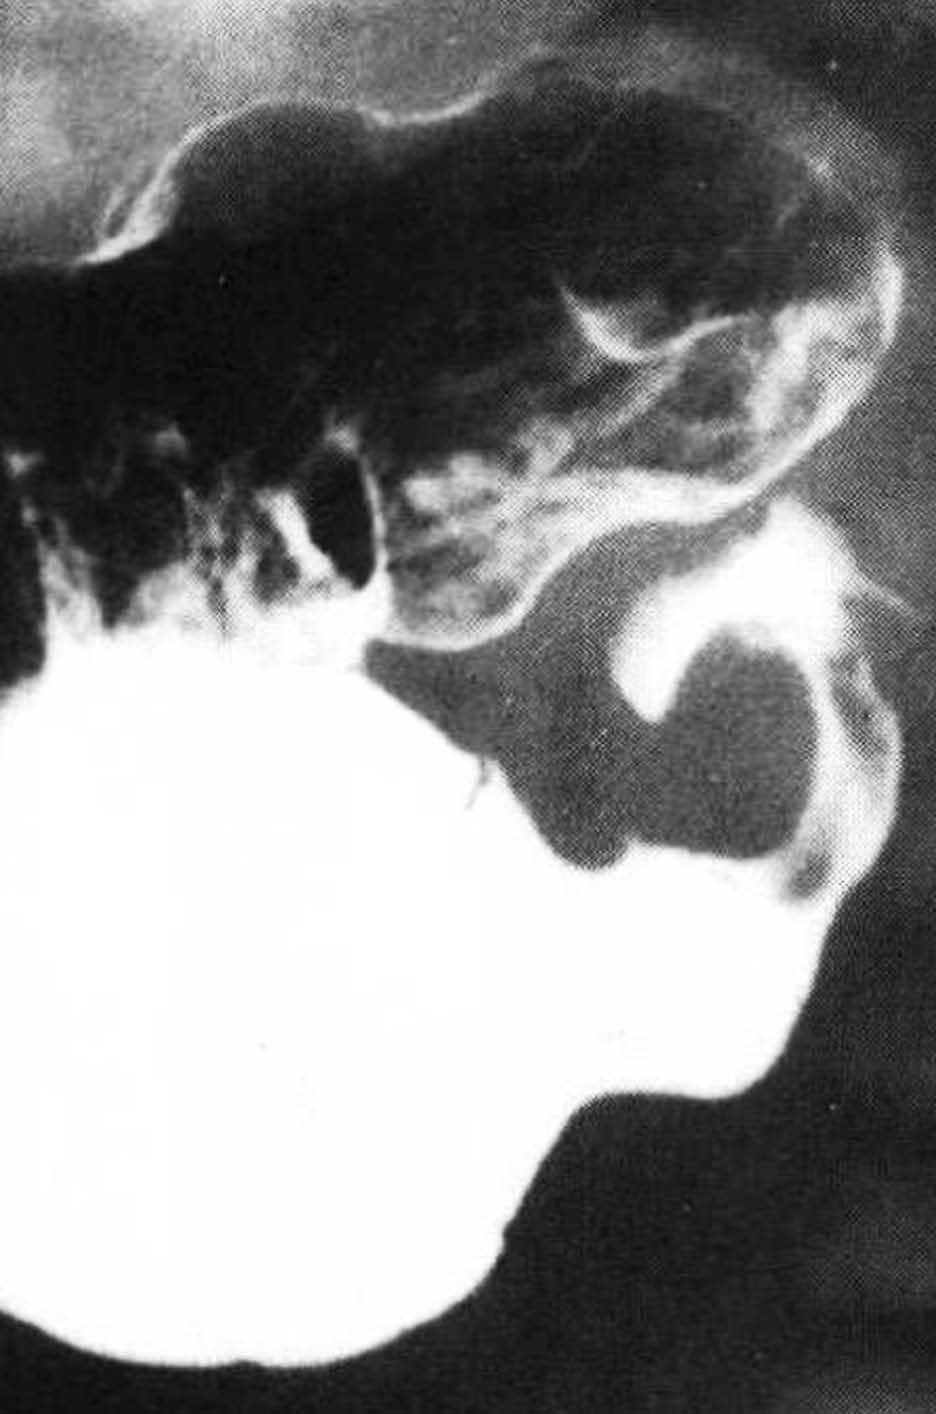
\includegraphics{./images/Image00265.jpg}
 \captionsetup{justification=centering}
 \caption{幽门肌肥厚}
 \label{fig5-3-4}
  \end{figure} 

\textbf{【病史摘要】}
 女性,40岁。右上腹部饱胀数月,无明显疼痛,时有恶心、呕吐。体格检查:中等体质,腹软,肝、脾未及,右上腹无明显压痛,心、肺阴性。

\textbf{【X线表现】}
 胃钡透示:胃幽门管细而长,其纵行粘膜皱襞显示呈双轨征,十二指肠球基底部形成蘑菇征。

\textbf{【X线诊断】}  幽门肌肥厚。

\textbf{【评  述】}
 本病是胃幽门环肌高度肥厚所致。多见于成年人。腹痛、腹胀、恶心、呕吐等为常见症状。幽门肌肥厚X线表现主要有:①钡剂通过狭窄的幽门管,幽门管显示狭窄而延长,呈线条状。②由于肥大的幽门肌终止于十二指肠球基底部,造成肥大的环形肌肉压迫球部基底部形成蘑菇征。③钡剂进入狭窄的幽门管,当充盈不全时似一个细长的鸟嘴突向十二指肠球部。④狭窄之幽门管纵行的粘膜皱襞显影形成双轨征。X线诊断应与幽门痉挛鉴别,但幽门痉挛无以上X线征象,确诊并不困难。

\subsection{胃息肉}

\begin{figure}[!htbp]
 \centering
 
\includegraphics{./images/Image00266.jpg}
 \captionsetup{justification=centering}
 \caption{胃息肉}
 \label{fig5-3-5}
  \end{figure} 

\textbf{【病史摘要】}
 女性,43岁。上腹部疼痛不适,无食欲减退、嗳气、反酸。体格检查:腹软,上腹部轻压痛,肝、脾未及,心、肺阴性。

\textbf{【X线表现】}
 胃钡透示:胃窦部圆形充盈缺损,边缘整齐锐利,表面光滑,周围胃壁柔软,无僵硬,蠕动正常。

\textbf{【X线诊断】}  胃息肉(胃窦部)。

\textbf{【评  述】}
 本病常为单发,也可多发,多发者称胃息肉病。典型X线表现呈圆形或类圆形充盈缺损突入于胃腔,有蒂或无蒂,直径一般小于2cm。多见于胃窦及胃体下部,幽门前区带蒂息肉可脱入十二指肠内。息肉表面光滑整齐。组织学检查可分为腺瘤性息肉及增生性息肉两类。腺瘤性息肉多位于胃窦部,常伴萎缩性胃炎,可分为腺瘤及乳头状瘤,后者可呈菜花状。增生性息肉是在慢性胃炎基础上发生的,很少超过1cm。腺瘤性息肉被认为是癌前期病变,可与胃癌同时存在。临床一般多无症状,少数可有上腹部不适疼痛。带蒂者可随蠕动或压迫而移位。在幽门前区者突入十二指肠时,表现为十二指肠球部的充盈缺损,充盈加压检查或双重造影法可显示其带蒂。乳头状腺瘤可不规则。息肉应与息肉样癌鉴别,息肉样癌的充盈缺损一般多大于2cm,形态不规则,表面粗糙,肿瘤与胃壁交界欠清,一般无蒂。

\subsection{胃窦炎}

\begin{figure}[!htbp]
 \centering
 
\includegraphics{./images/Image00267.jpg}
 \captionsetup{justification=centering}
 \caption{胃窦炎伴幽门痉挛}
 \label{fig5-3-6}
  \end{figure} 

\textbf{【病史摘要】}
 女性,40岁。左上腹部不适3个月余,食欲减退,时有恶心、呕吐。体格检查:腹软,肝、脾未及,上腹压痛,心、肺阴性。

\textbf{【X线表现】}
 胃窦部粘膜皱襞增粗、紊乱,幽门管痉挛,钡剂通过幽门管稍受阻,胃窦壁轮廓见锯齿状影,胃窦壁柔软,蠕动增强。

\textbf{【X线诊断】}  胃窦炎伴幽门痉挛。

\textbf{【评  述】}
 胃窦炎为局限于胃窦部的慢性炎症,可为浅表性或萎缩性,十分常见。轻症无阳性X线表现。常见的异常征象有:胃窦部粘膜皱襞增粗、紊乱。正常的胃窦部粘膜皱襞较体部细小,胃窦炎时可增大。紊乱的粘膜皱襞,即使在半收缩状态也呈横行,使窦部轮廓呈光滑的锯齿状。增粗的粘膜皱襞可呈息肉状,并随蠕动、舒缩或压迫而变形。肌层受累者,窦部呈向心性狭窄,但仍可见呈纵行的粘膜皱襞。窦部因环形及纵行肌的收缩与增厚而变短、变窄,其界线呈渐进性或较清楚。肌层的痉挛或增厚可致幽门前区小弯侧呈弧形压迫。幽门管可变窄并伸长。粘膜下层的增厚,使粘膜活动度增加,易形成粘膜脱垂。胃小沟及胃小区增宽、增大。窦部痉挛及分泌功能增强为常见的功能异常。胃窦炎常致窦部狭窄而应与胃窦癌鉴别。胃窦炎的狭窄,形态可变、粘膜皱襞存在、轮廓也较整齐,而胃窦癌表现为胃窦狭窄壁僵硬,与正常胃段分界陡峭呈截断征象,粘膜皱襞破坏,典型者可呈肩胛征。

\subsection{慢性胃炎}

\begin{figure}[!htbp]
 \centering
 
\includegraphics{./images/Image00268.jpg}
 \captionsetup{justification=centering}
 \caption{慢性胃炎}
 \label{fig5-3-7}
  \end{figure} 

\textbf{【病史摘要】}
 男性,65岁。上腹部疼痛不适,嗳气、反酸、餐后饱胀数月。体格检查:腹软,肝、脾未及,右上腹压痛,心、肺阴性。

\textbf{【X线表现】}
 胃钡透示:胃体、胃窦粘膜皱襞增粗、肥厚、紊乱,部分呈弯曲、交叉状,胃体、胃窦处胃壁毛糙,压迫后胃壁柔软,胃蠕动正常。

\textbf{【X线诊断】}  慢性胃炎。

\textbf{【评  述】}
 本病为成人常见病,病因尚未完全明确。病理上慢性胃炎可分为慢性浅表性胃炎和慢性萎缩性胃炎及慢性肥厚性胃炎。慢性胃炎时粘膜充血、水肿、炎性细胞浸润及纤维结缔组织增生。轻微者肉眼难以发现,较重者粘膜皱襞增粗、迂回呈脑回状;部分萎缩性胃炎粘膜层萎缩变薄,皱襞细小。慢性胃炎病程较长,可长期反复发作。一般临床表现为食欲不振、腹痛、腹胀、恶心、呕吐、嗳气等。萎缩性胃炎可有贫血、营养不良、腹泻等表现。慢性胃炎的X线表现主要为粘膜皱襞增粗、迂曲、走行异常、失去与小弯平行的特点,体部及窦部粘膜皱襞超过0.5cm,甚至超过1cm;充盈像,因粘膜皱襞增粗、迂曲而使小弯侧凹凸不平,但形态不变,蠕动正常,而不致误为肿瘤。除上述外,还可见分泌功能增强及蠕动增强等变化。部分萎缩性胃炎粘膜皱襞纤细、稀少,服钡或双重造影的气体稍多,胃呈轻度扩张时,皱襞即可变平,甚至大弯侧也可变得光滑。胃小区增大,多数大于3mm,而且粗糙不规则。慢性胃炎常与溃疡并存,而有相应X线征。

\subsection{腐蚀性胃、十二指肠炎}

\begin{figure}[!htbp]
 \centering
 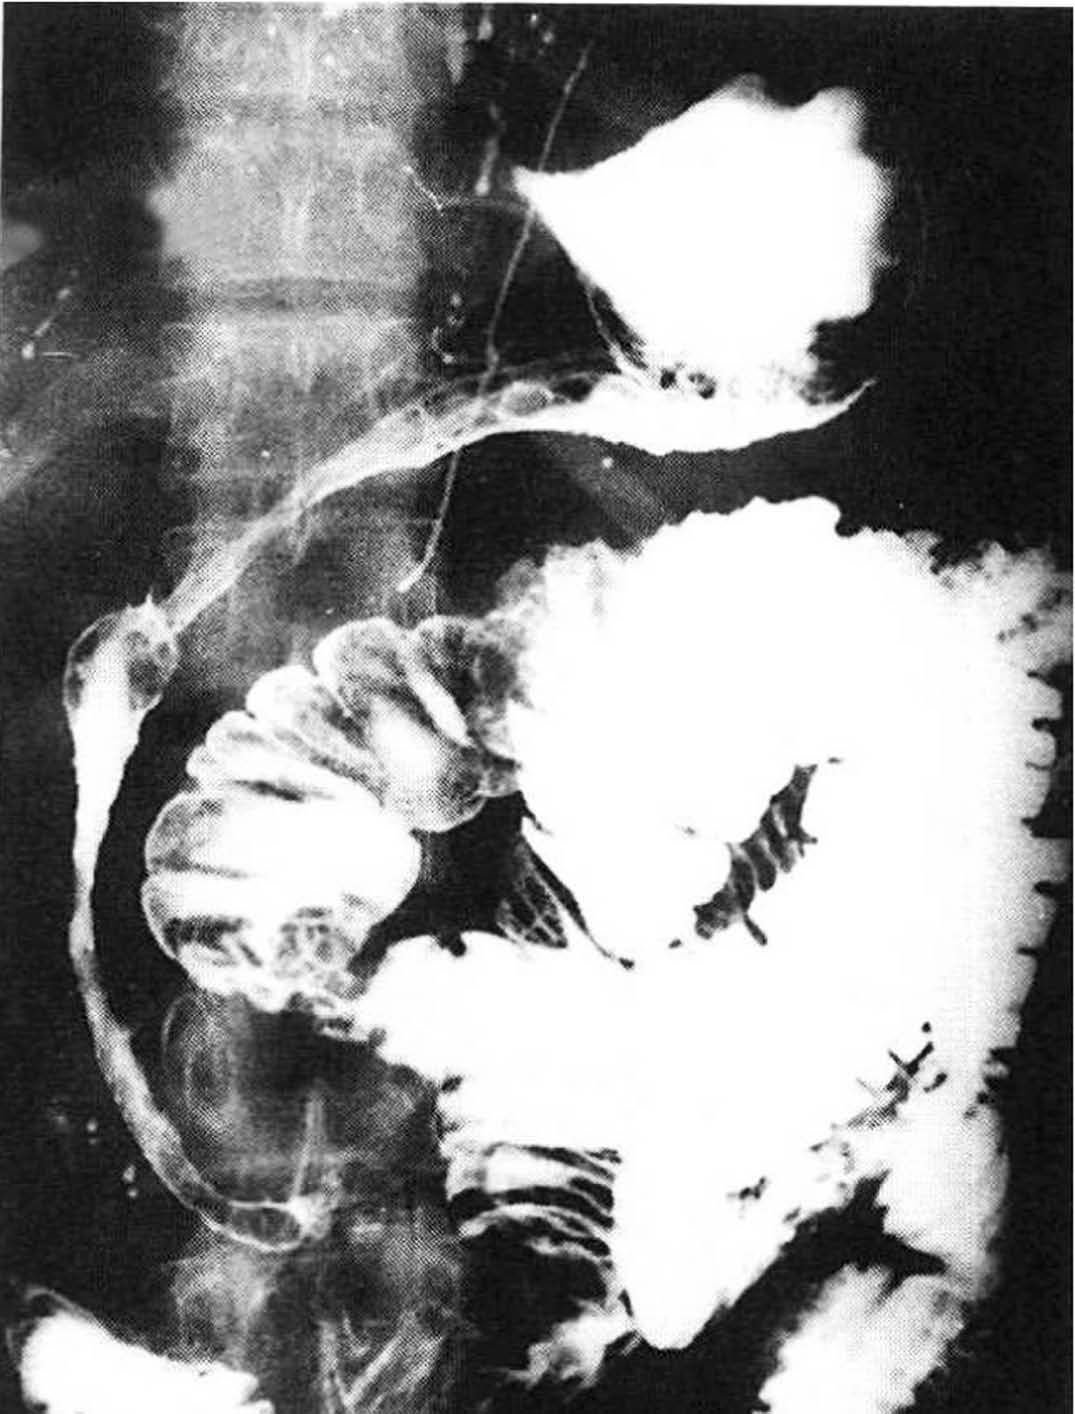
\includegraphics{./images/Image00269.jpg}
 \captionsetup{justification=centering}
 \caption{腐蚀性胃、十二指肠炎}
 \label{fig5-3-8}
  \end{figure} 

\textbf{【病史摘要】}
 女性,35岁。因进食时吞咽困难、呕吐频繁伴胸痛入院,数月前有硫酸误服致上消化道灼伤史。

\textbf{【X线表现】}
 胃钡透示:胃、十二指肠高度狭窄、壁僵硬,粘膜皱襞消失,部分边缘可见针尖样突出的小溃疡。

\textbf{【X线诊断】}  腐蚀性胃、十二指肠炎。

\textbf{【评  述】}
 吞服酸性腐蚀剂类物质易损伤食管、胃、十二指肠,若腐蚀剂浓度高、量大、接触时间长,可引起食管、胃、十二指肠以及空肠的烧灼性炎症。病理改变主要为粘膜及粘膜下层坏死。溃疡形成,晚期纤维瘢痕形成导致不同程度各种各样的狭窄。X线表现早期改变为胃粘膜皱襞粗大、水肿,可有溃疡龛影。胃蠕动消失。晚期可见胃腔狭窄呈漏斗状,胃壁边缘不规则如锯齿状,胃幽门瘢痕性狭窄。由于有患者误服腐蚀剂病史,故诊断一般不难。

\subsection{胃粘膜脱垂}

\begin{figure}[!htbp]
 \centering
 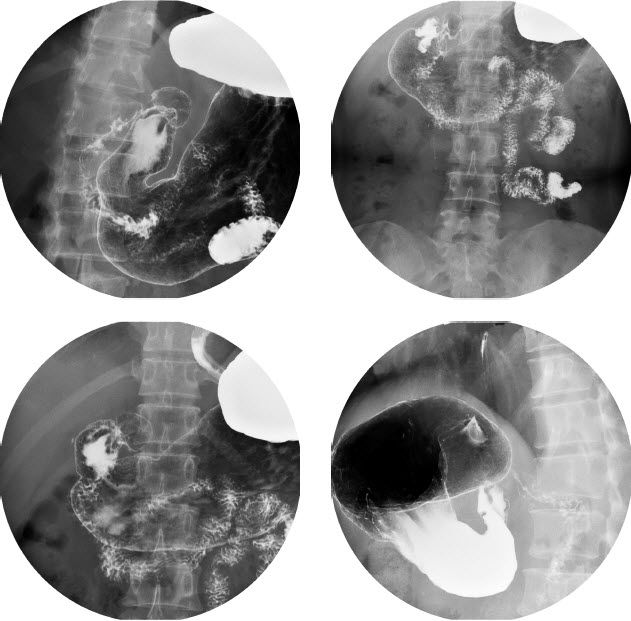
\includegraphics{./images/Image00270.jpg}
 \captionsetup{justification=centering}
 \caption{胃粘膜脱垂}
 \label{fig5-3-9}
  \end{figure} 

\textbf{【病史摘要】}
 男性,45岁。因上腹部不适,嗳气、反酸入院。体格检查:腹软,肝、脾未及,右上腹压痛,心、肺阴性。

\textbf{【X线表现】}
 胃钡透示:幽门管变宽,内见条状平行胃粘膜皱襞,十二指肠球部呈伞状,基底部见类圆形充盈缺损影。

\textbf{【X线诊断】}  胃粘膜脱垂。

\textbf{【评  述】}
 胃粘膜进入十二指肠称为胃粘膜脱垂,常为可复性。常见症状为上腹部疼痛,可随体位改变而缓解。X线表现随脱垂的粘膜数量及程度而异,一般可见幽门管增宽,其内可见条形皱襞。十二指肠球内见圆形或椭圆形充盈缺损,位于正中或呈偏侧性,随窦部的加压或体位的改变而时隐时现。球底一般呈伞状。诊断时应与幽门前区带蒂肿瘤脱入十二指肠相鉴别。后者形态、大小固定,不随压迫变形,回纳后,幽门前区仍可见之。钡餐检查时,当怀疑有胃粘膜脱垂可能时,需要重点注意的是:①应充分利用立位检查或腹部加压检查。②尽可能使球部纵轴走行方向与X线方向垂直。③胃窦处于舒张状态时摄片。④诊断胃粘膜脱垂时,必须肯定球底部之阴影为胃粘膜皱襞,除外体位不当造成的假象。

\subsection{胃溃疡}

\begin{figure}[!htbp]
 \centering
 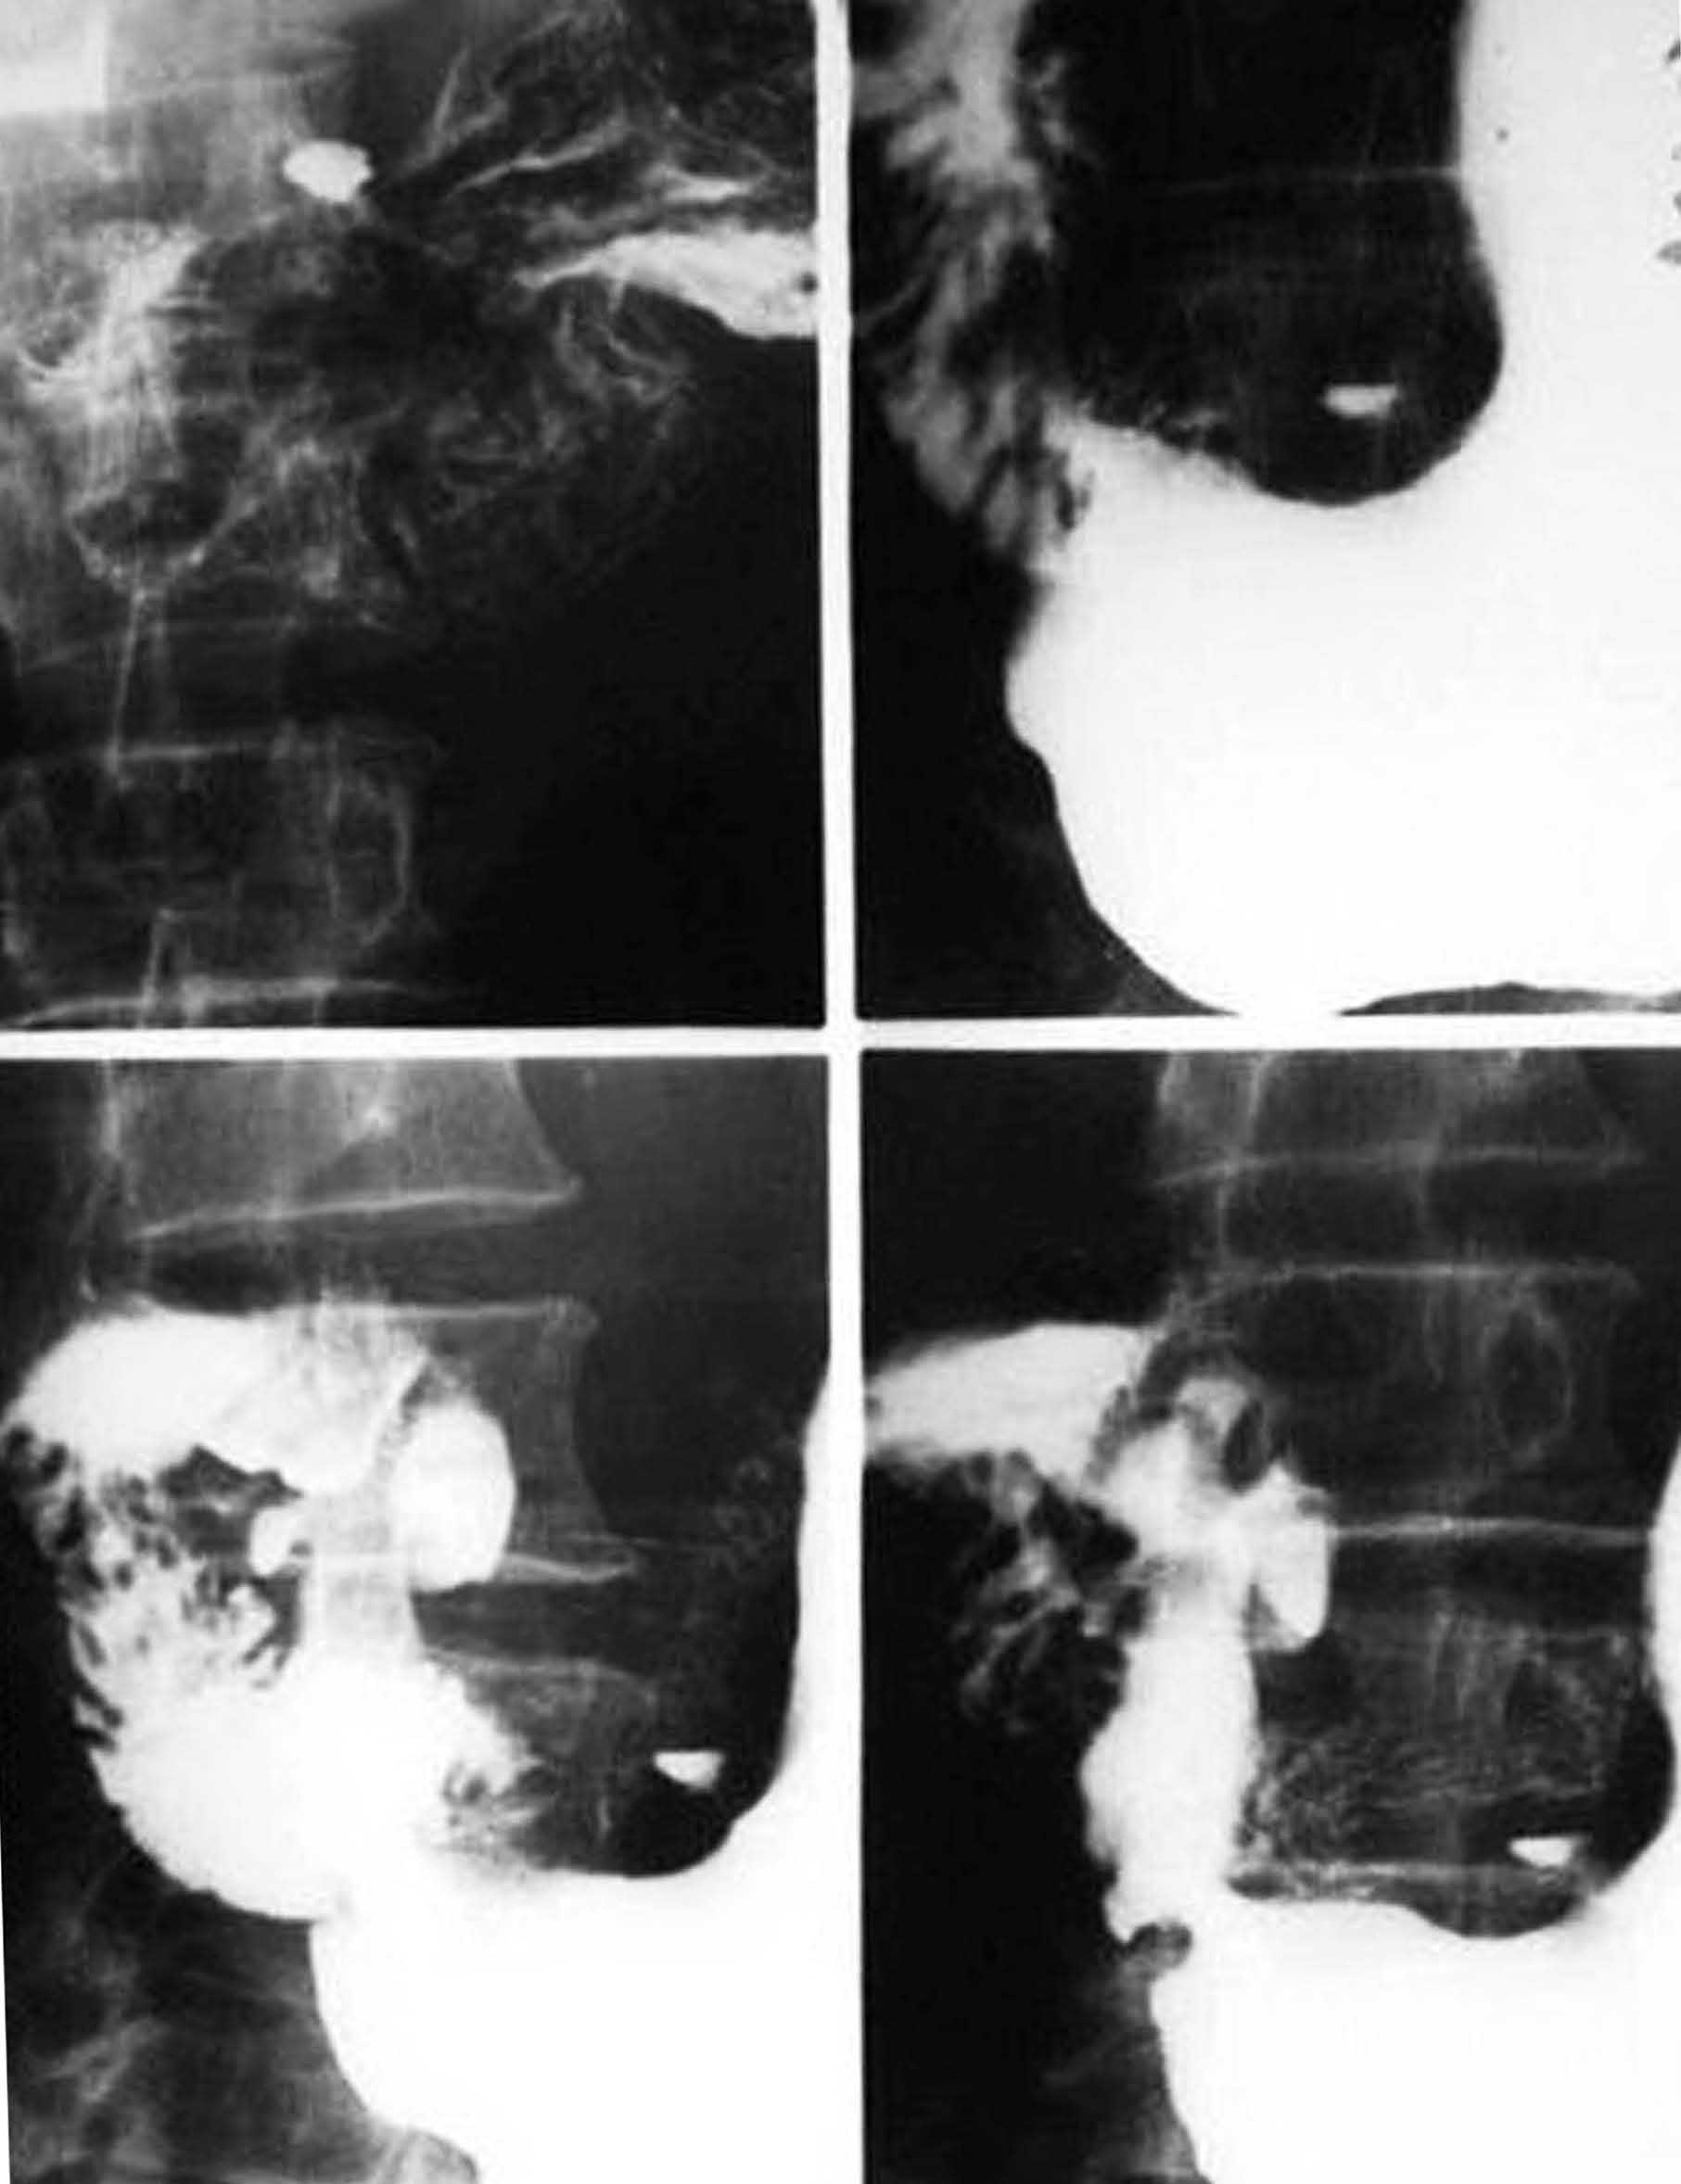
\includegraphics{./images/Image00271.jpg}
 \captionsetup{justification=centering}
 \caption{胃角溃疡}
 \label{fig5-3-10}
  \end{figure} 

\textbf{【病史摘要】}
 男性,55岁。上腹部不适数年,进餐后可缓解,近一周上腹部疼痛加重,具有周期性及节律性,伴恶心、呕吐、嗳气、反酸。体格检查:腹软,肝、脾未及,右上腹压痛明显,心、肺阴性。

\textbf{【X线表现】}
 胃钡透示:胃角处见一突出于胃腔外的乳头状影,基底部见狭颈征,龛周粘膜皱襞纠集。

\textbf{【X线诊断】}  胃角溃疡。

\textbf{【评  述】}
 本例经胃镜检查病理证实为胃体小弯侧溃疡。上消化道钡餐造影显示胃角处见一突出于胃腔外的乳头状影,基底部见狭颈征,龛周粘膜皱襞纠集,符合良性胃溃疡的X线表现,故诊断不难。需要鉴别的是胃小弯侧恶性溃疡,后者以壁龛及邻近胃壁变化为主要表现。龛影多数较浅而大,形态多不规则,具有特征性的为口部指压迹征和裂隙征,与良性溃疡平坦的口部出现的狭颈征、项圈征对比分明。

\subsection{幽门管溃疡}

\begin{figure}[!htbp]
 \centering
 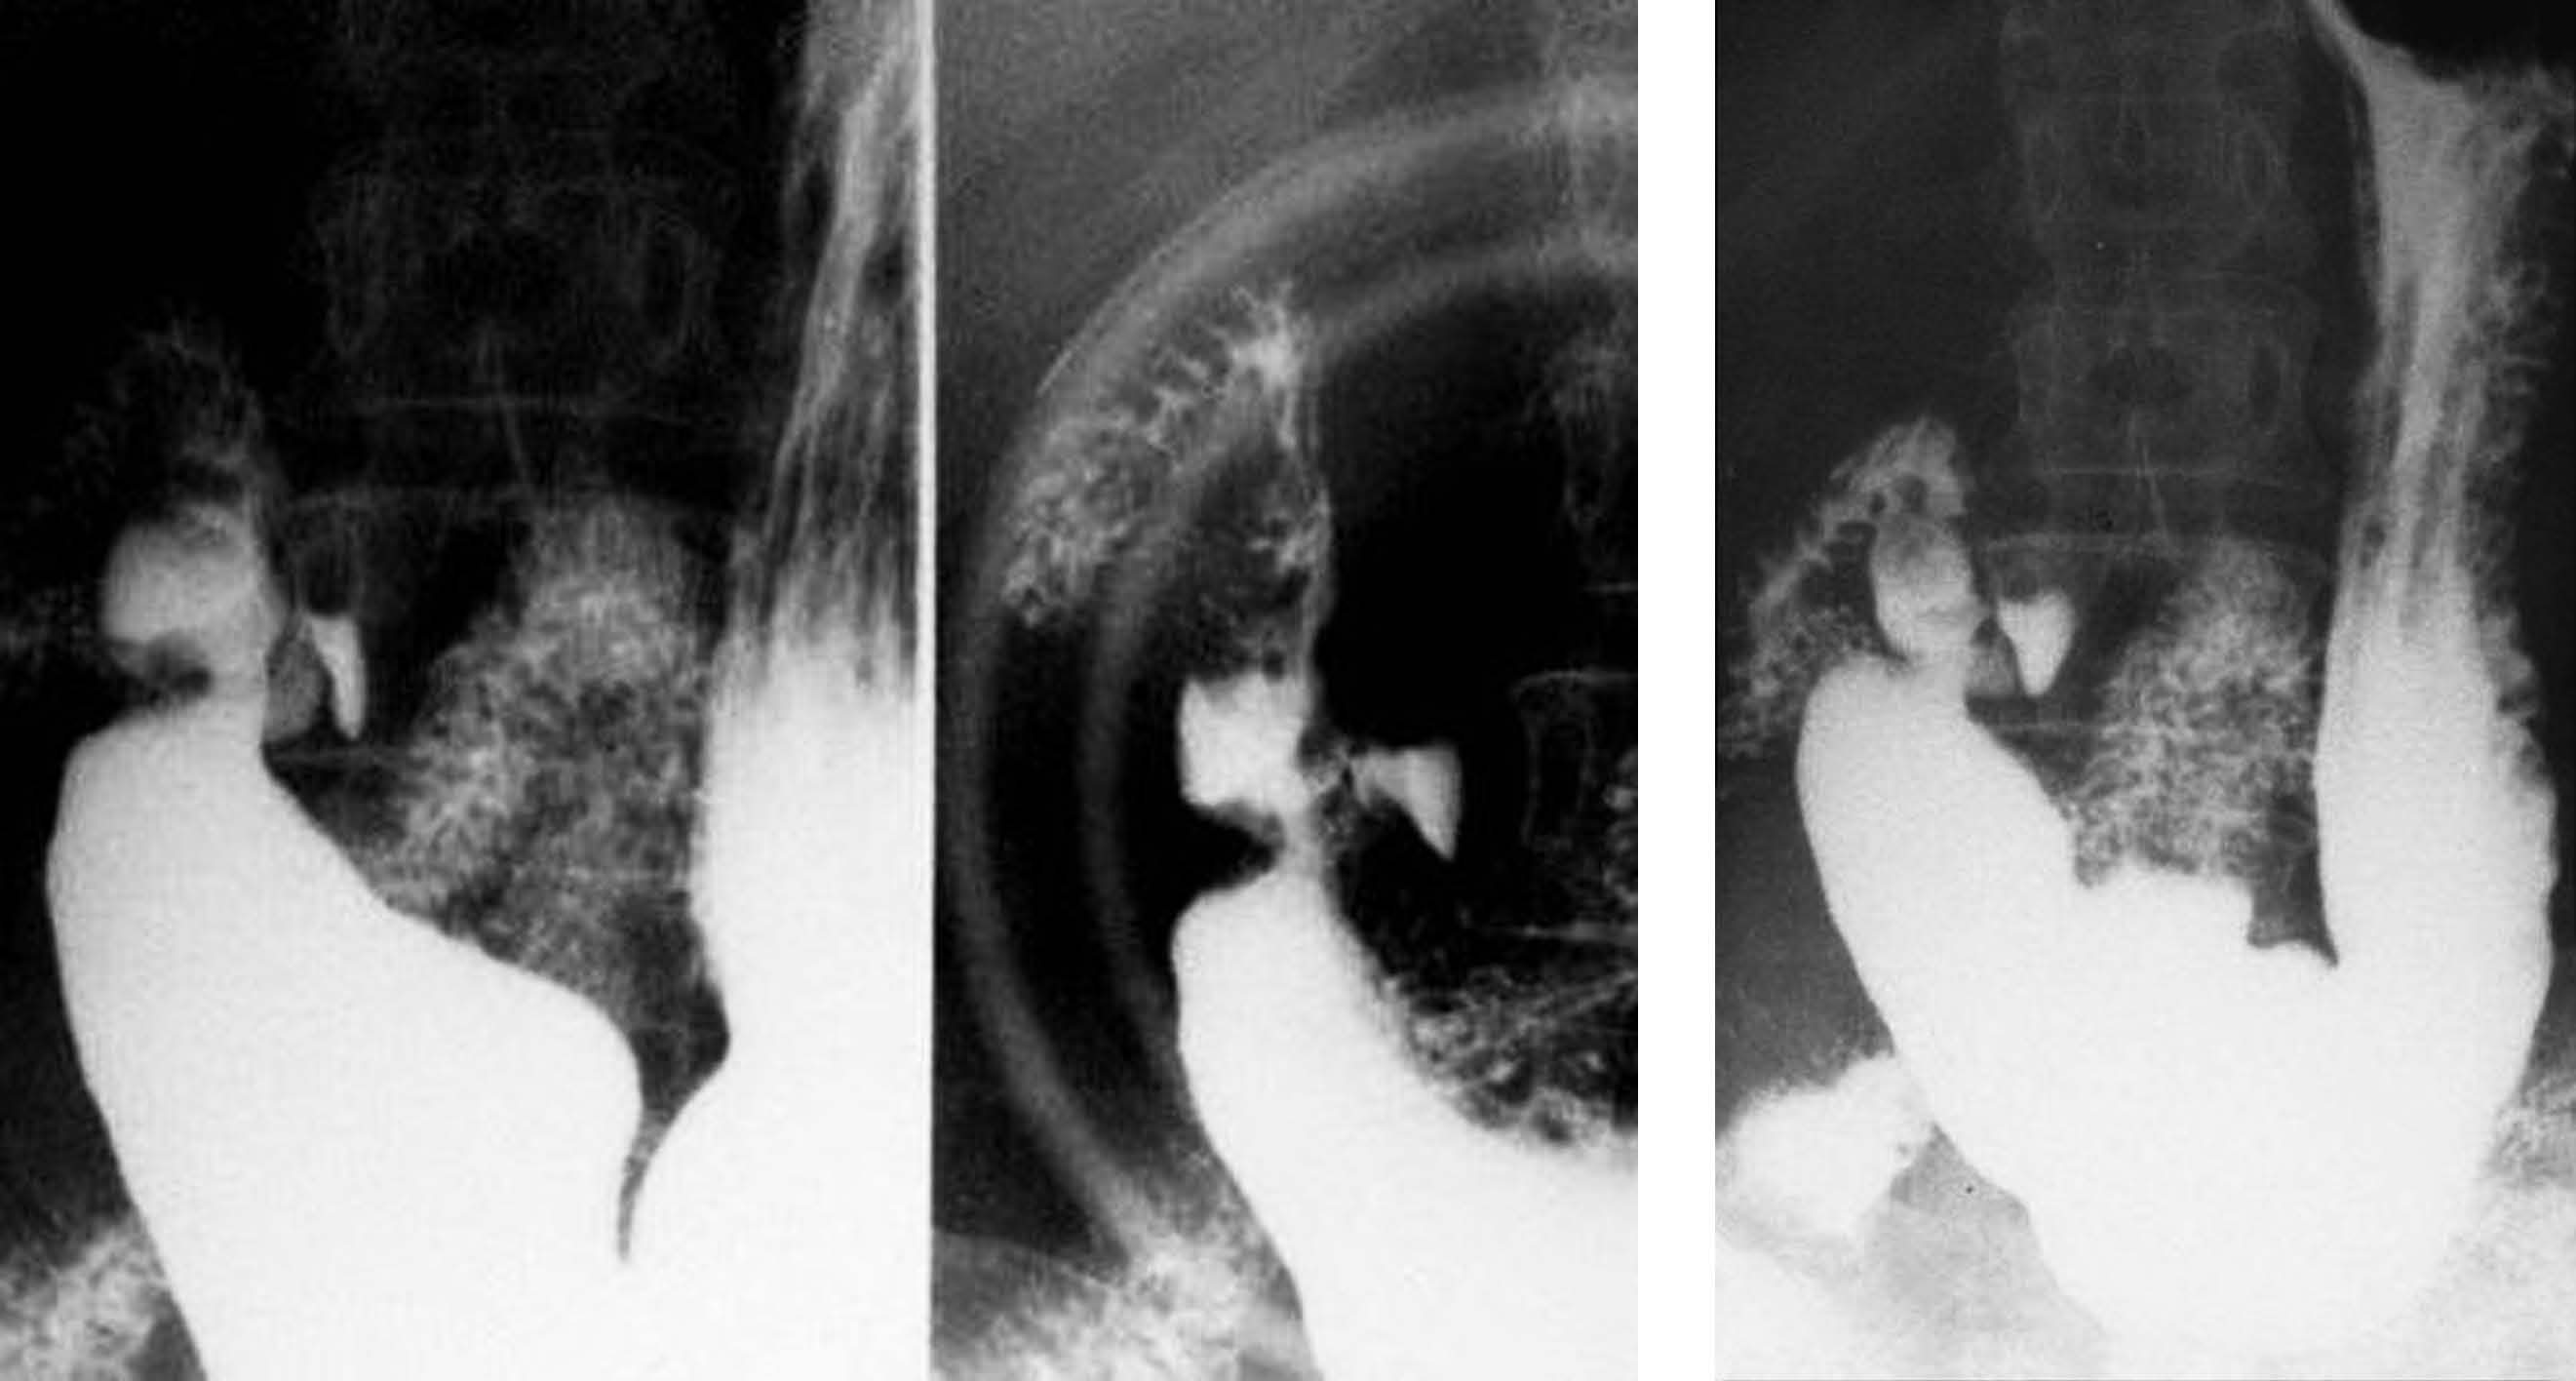
\includegraphics{./images/Image00272.jpg}
 \captionsetup{justification=centering}
 \caption{幽门管溃疡}
 \label{fig5-3-11}
  \end{figure} 

\textbf{【病史摘要】}
 男性,45岁。上腹部疼痛伴嗳气、反酸2个月,近期疼痛加重伴呕吐。体格检查:腹软,肝、脾未及,右上腹压痛明显,心、肺阴性。

\textbf{【X线表现】}
 上消化道钡餐造影示:幽门管区见突出于胃腔外的三角形龛影,底部狭窄,呈项圈征。

\textbf{【X线诊断】}  幽门管溃疡。

\textbf{【评  述】}
 本病为常见病,发病机制不甚明了,好发年龄为20~50岁。胃溃疡常单发,多在小弯及胃角处,其次为胃窦部,其他部位少见。病理改变主要为胃壁溃烂缺损,形成壁龛。溃疡先从粘膜开始并逐渐侵及粘膜下层,常深达肌层。X线检查是胃溃疡的重要检查方法,尤其是气钡双重造影,可显示小而表浅的溃疡。溃疡病的X线表现,可分为直接与间接征象,前者为X线诊断的主要依据。

1.直接征象 龛影为溃疡充钡后在X线上的反映,是溃疡的直接征象。在正位像上,呈圆形或类圆形影;如果溃疡内的钡剂较少,仅四周壁附薄层钡剂,则呈环形,即所谓环形龛影。在切线位上,龛影突出于胃轮廓之外,多呈乳头状,或为半圆形及锥形。边缘光滑整齐,底部平整。在切线位上还可显示:①粘膜线:为溃疡口部宽1~2mm的透光线影,见于口部的上缘、下缘或横贯整个口部。②狭颈征:龛影口部明显狭小,使龛影犹如一个狭长的颈。③项圈征:龛影口部的透明带,宽0.5~1cm,犹如一项圈。粘膜线、狭颈征、项圈征皆为溃疡周围炎性水肿所致。④粘膜纠集,溃疡周围的粘膜皱襞,因瘢痕收缩向壁龛均匀性纠集,直达龛影,呈星芒状。

2.间接征象 下述X线表现常见于胃溃疡,也可因胃癌所致,不具有特异性,但在综合分析时有一定价值。①胃小弯短缩:是小弯侧溃疡纤维组织增生,牵拉幽门及贲门靠近。②胃大弯侧指状切迹:胃小弯侧溃疡,因环形肌痉挛性收缩,在溃疡的对侧可见一指状切迹,立位时明显。③幽门梗阻及狭窄:幽门及其邻近部的溃疡可致幽门持久性痉挛,或因瘢痕形成而使幽门梗阻。X线可见空腹胃潴留液增多,幽门管狭小,钡剂通过困难。④胃液分泌增多:在无幽门梗阻的情况下,出现少至中等量的胃内空腹潴留液,使钡剂不易附着于胃壁而难以显示粘膜皱襞。⑤胃蠕动的变化:蠕动增强或减弱,张力增高或降低,排空加速或延缓。⑥局限性压痛:龛影部位常有明显的局限性压痛。

\subsection{穿透性溃疡}

\begin{figure}[!htbp]
 \centering
 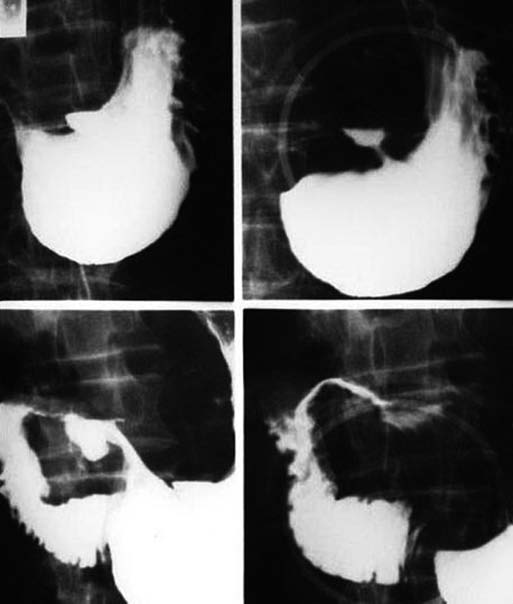
\includegraphics{./images/Image00273.jpg}
 \captionsetup{justification=centering}
 \caption{胃角穿透性溃疡}
 \label{fig5-3-12}
  \end{figure} 

\textbf{【病史摘要】}
 男性,48岁。胃溃疡病史3年,近一周来上腹部疼痛加剧伴恶心、呕吐。体格检查:贫血貌,上腹部拒按,压痛明显,心、肺阴性。

\textbf{【X线表现】}
 上消化道钡餐检查示:胃小弯侧腔外见一1.8cm×2.0cm大小囊袋状影,轮廓尚光整,颈部狭长,狭颈征明显。

\textbf{【X线诊断】}  胃角穿透性溃疡。

\textbf{【评  述】}
 本例患者经手术证实为穿透性溃疡。穿透性溃疡为胃溃疡的特殊类型,其特点为龛影大而深,其深度与大小均超过1.0cm,形如囊袋状,狭颈征显著。需注意此征象与较大的胃憩室相鉴别:胃憩室发生部位以胃底贲门区后壁为多见,憩室内可显示胃粘膜皱襞影;穿透性溃疡X线表现如周围较广泛的水肿带以及粘膜皱襞向溃疡口部纠集征象与胃憩室不同。胃溃疡根据以上典型表现,诊断一般不难。但有时因瘢痕组织的不规则增生或溃疡比较扁平者易与恶性溃疡混淆。良性溃疡和恶性溃疡的鉴别诊断,应从龛影的形态、溃疡的位置、溃疡的口部、周围粘膜皱襞的情况、邻近胃壁的柔软与蠕动等多方面综合分析,详见下表。

胃良、恶性溃疡的X线鉴别诊断

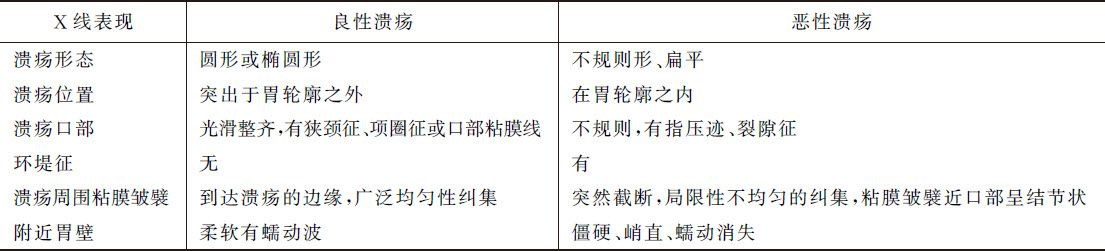
\includegraphics{./images/Image00274.jpg}

\subsection{胃平滑肌瘤}

\begin{figure}[!htbp]
 \centering
 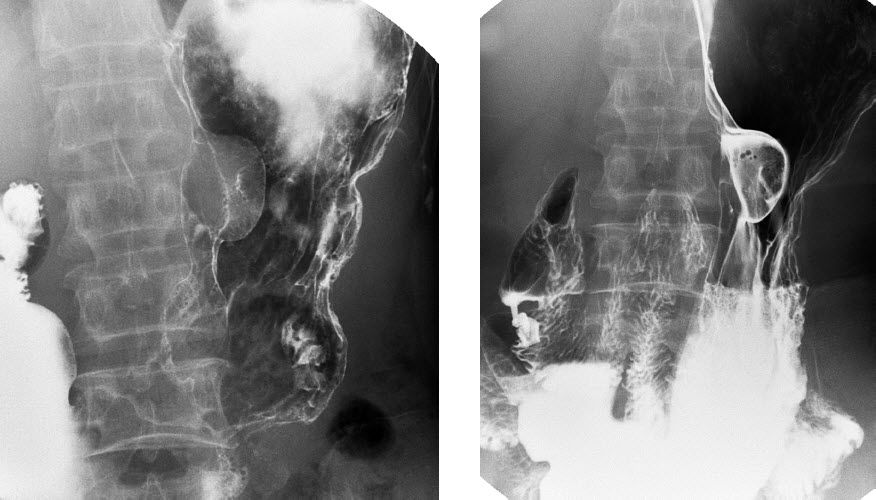
\includegraphics{./images/Image00275.jpg}
 \captionsetup{justification=centering}
 \caption{胃平滑肌瘤}
 \label{fig5-3-13}
  \end{figure} 

\textbf{【病史摘要】}
 女性,42岁。吞咽困难半年余,无明显疼痛,无消瘦。体格检查:腹软,肝、脾未及,腹部无压痛,心、肺阴性。

\textbf{【X线表现】}
 上消化道钡餐造影示:胃贲门下部见一类圆形充盈缺损,边缘光滑清晰,中央部可见小钡斑。

\textbf{【X线诊断】}  胃平滑肌瘤。

\textbf{【评  述】}
 本例患者经手术治疗病理证实为胃平滑肌瘤。胃平滑肌瘤来源于中胚层组织,大多在5cm以下,可分为胃内型、胃壁型、胃外型。X线表现主要有:①胃内隆起性病变:正面呈圆形、椭圆形,位于大、小弯者显示其侧面像为半圆形。充盈像时呈边缘光滑的充盈缺损。②粘膜皱襞:肿瘤表面被附粘膜,可见粘膜皱襞通过肿物征象,粘膜被抬起形成桥形皱襞,或被推开形成粘膜皱襞的躲避、迂回征象。肿瘤较大时,皱襞受压变薄、变平以致消失。③中心凹陷:肿瘤表面,尤其顶部常形成小凹陷,造影时出现小钡斑,即所谓的中心性凹陷。④肿瘤触诊:平滑肌瘤较硬,压之无变形。⑤钙化:平滑肌瘤可发生钙化,X线检查可见钙化斑。⑥周围改变:平滑肌瘤对周围无浸润,胃轮廓无僵硬。⑦恶性变:平滑肌瘤可恶变成为肉瘤。一般肿瘤较大、形态不规则、中心溃疡大而深又不规则时,应考虑恶变的可能性。

\subsection{胃淋巴瘤}

\begin{figure}[!htbp]
 \centering
 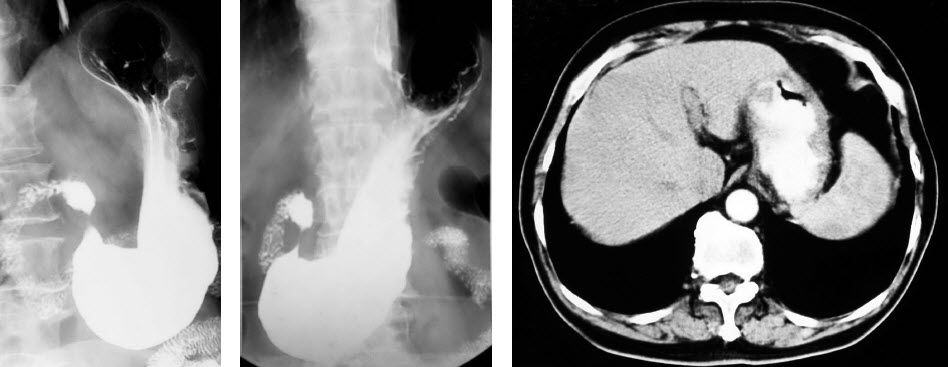
\includegraphics{./images/Image00276.jpg}
 \captionsetup{justification=centering}
 \caption{胃淋巴瘤}
 \label{fig5-3-14}
  \end{figure} 

\textbf{【病史摘要】}
 女性,40岁。上腹部不适3个月,食欲不振、消瘦,近期出现低热。体格检查:腹软,肝、脾未及,腹部无压痛,心、肺阴性,右侧锁骨上窝触及一类圆形肿块。

\textbf{【X线表现】}
 上消化道钡餐造影示:胃底大弯侧见不规则充盈缺损影,粘膜皱襞不规则增粗,胃壁柔韧度减弱,胃蠕动及收缩存在。CT检查示:胃底部胃壁局限性增厚,增强后均匀中度强化,壁柔软。

\textbf{【X线诊断】}  胃淋巴瘤。

\textbf{【评  述】}
 本例患者经手术治疗病理证实为胃淋巴瘤。胃肠道是淋巴结外淋巴瘤的最多见部位,最好累及胃。胃淋巴瘤可以是全身淋巴瘤的一部分,也可以是唯一的原发部位,多见于非霍奇金淋巴瘤。按形态学分类为:肿块型、溃疡型、浸润型和结节型。好发部位是胃体小弯侧和后壁。临床表现有上腹部疼痛、消瘦及上腹部肿块,可伴有全身淋巴瘤的其他表现。胃淋巴瘤X线常表现为局限性或广泛浸润性表现,前者为粘膜皱襞不规则、粗大,胃壁柔韧度消失,位于胃窦时呈漏斗状狭窄;后者为巨大粘膜皱襞的改变,排列紊乱,胃腔缩窄或变形,但其缩窄与变形程度不及浸润型胃癌。胃淋巴瘤缺乏特征性的X线表现,因此常不易与胃癌及其他肿瘤鉴别。但如下特征有助于本病的诊断:病变虽然广泛,但胃蠕动与收缩仍然存在,胃部病灶明显但临床一般情况较好,胃粘膜较广泛增粗,形态比较固定,临床有其他部位淋巴瘤的表现。

\subsection{早期胃癌(Ⅰ型)}

\begin{figure}[!htbp]
 \centering
 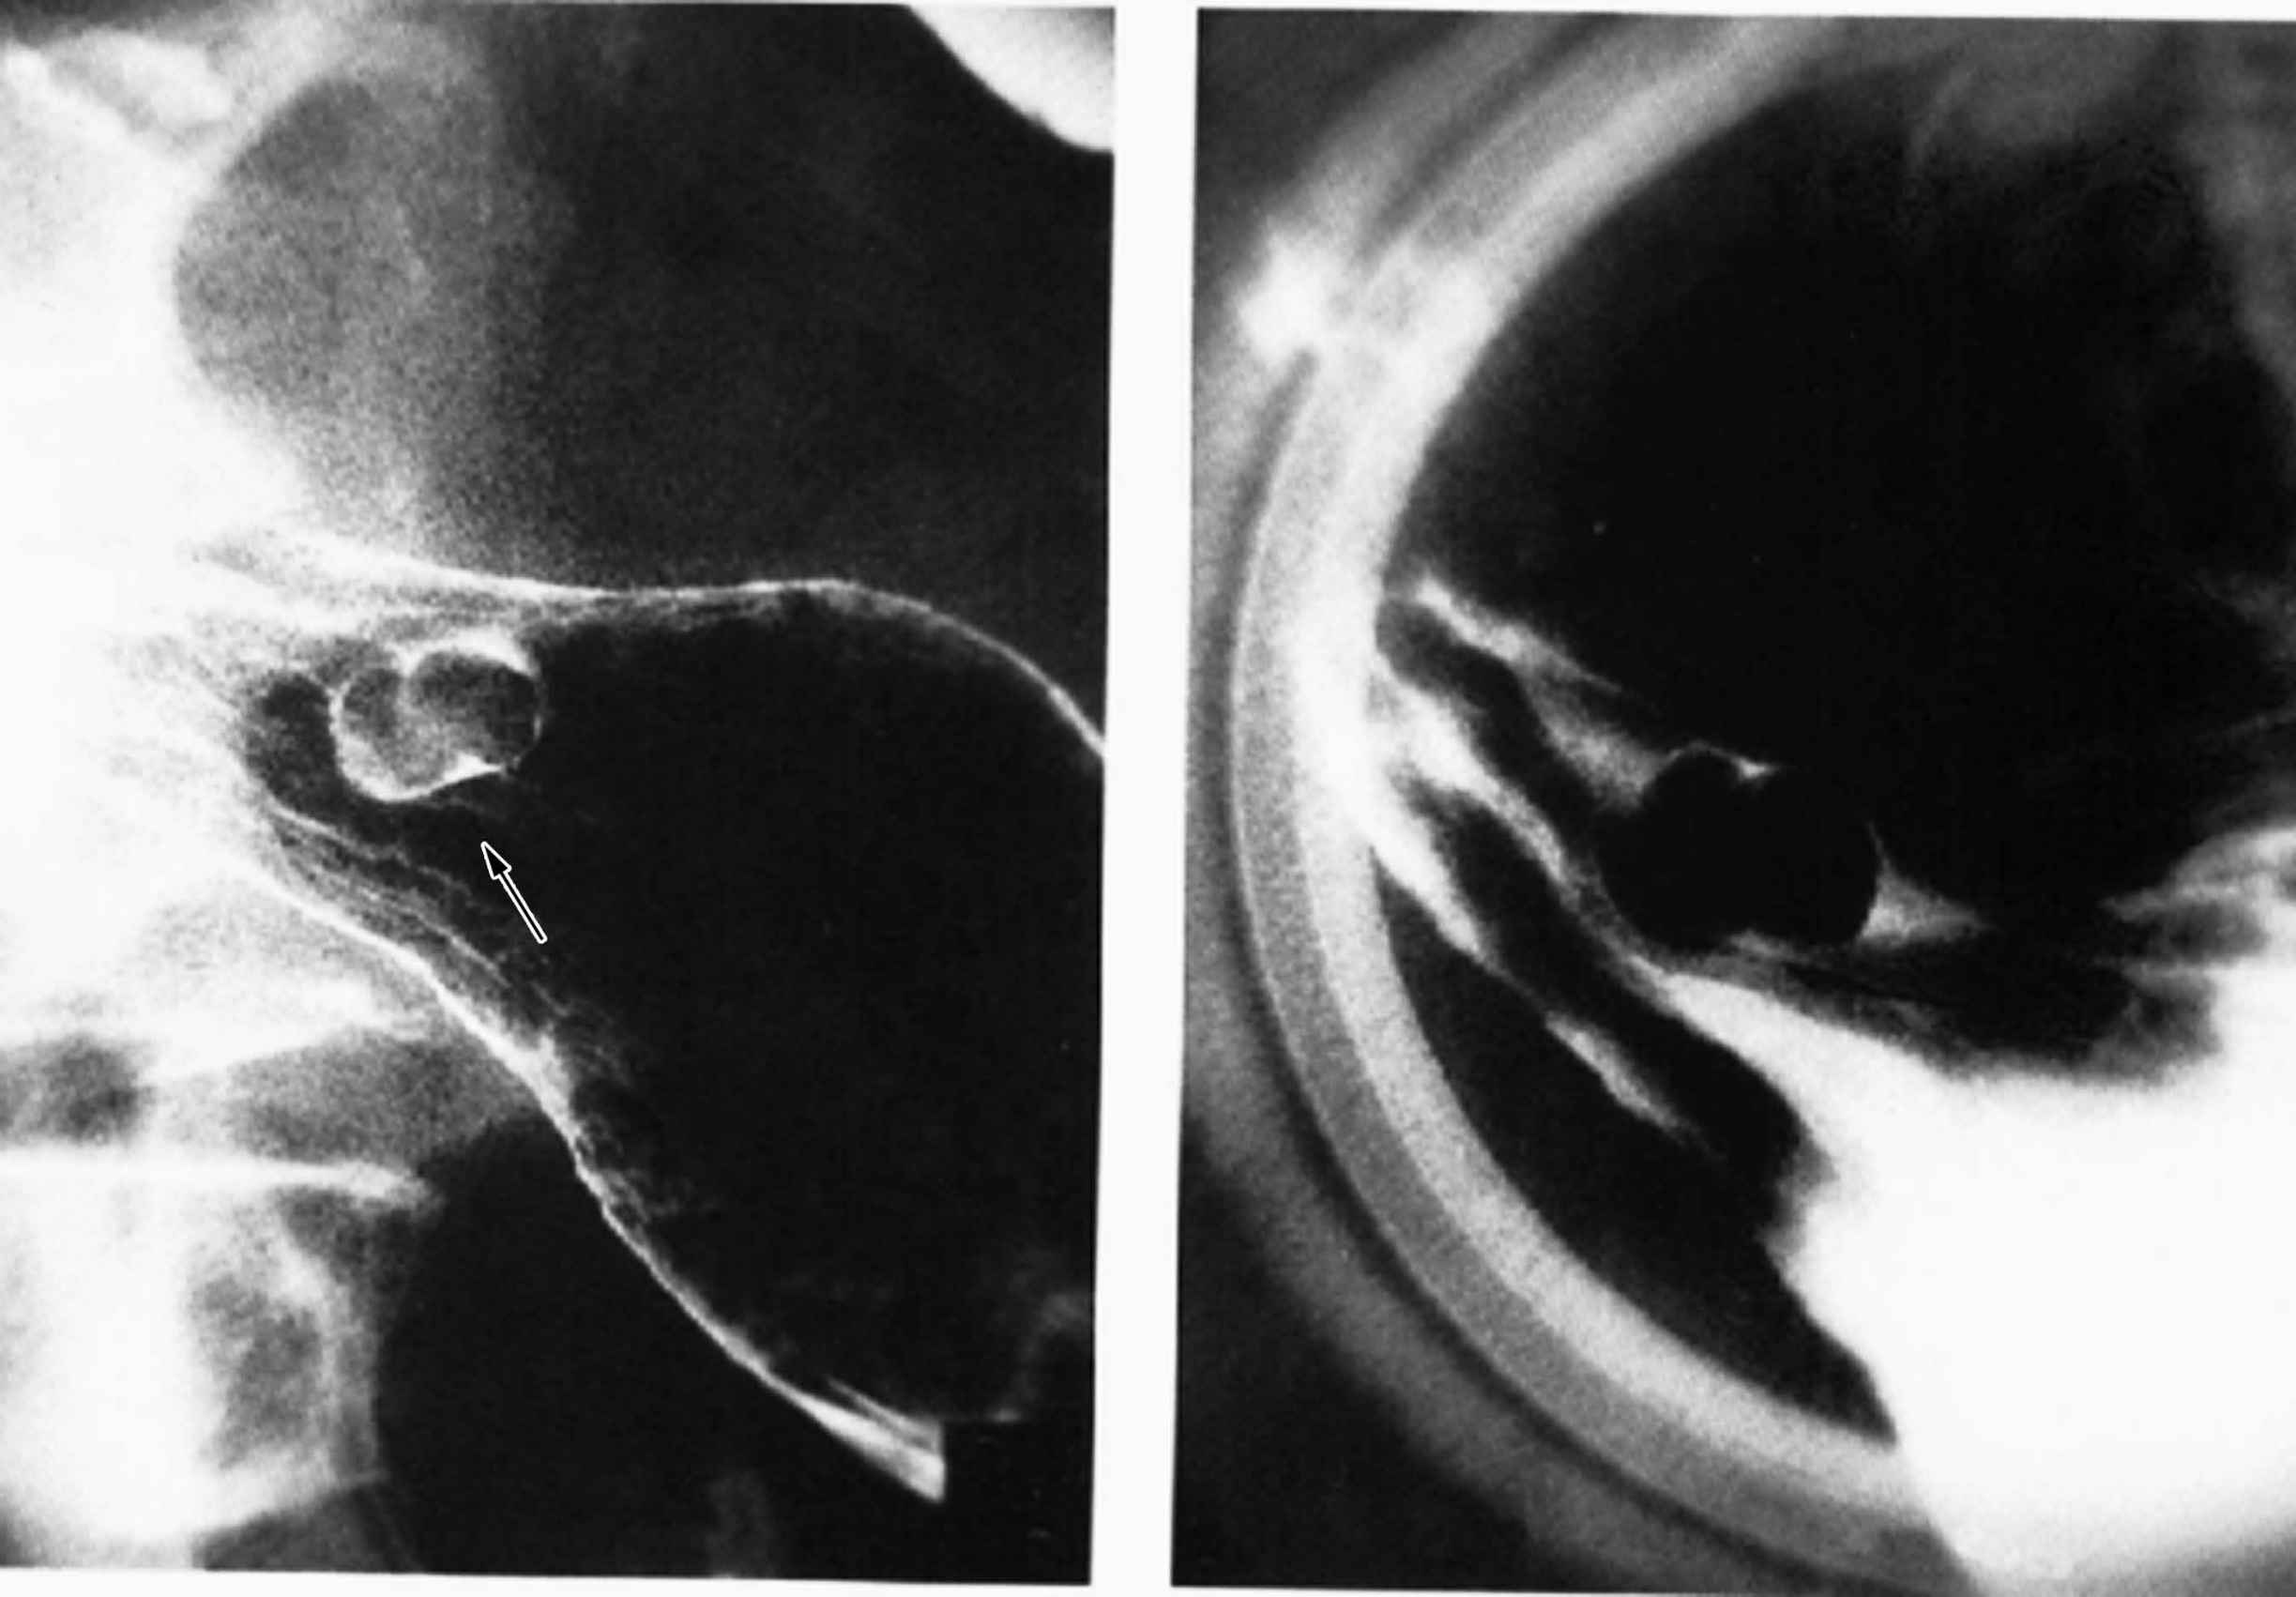
\includegraphics{./images/Image00277.jpg}
 \captionsetup{justification=centering}
 \caption{早期胃癌(Ⅰ型)}
 \label{fig5-3-15}
  \end{figure} 

\textbf{【病史摘要】}
 男性,61岁。上腹部不适、食欲不振、嗳气、反酸近1年,无黑便,无呕吐。体格检查:腹软,肝、脾未及,上腹部轻压痛,心、肺阴性。

\textbf{【X线表现】}
 上消化道钡餐造影示:胃窦部见一椭圆形充盈缺损影,边缘尚光整,周围粘膜皱襞中断破坏,基底部较宽,表面尚平坦,未见明显糜烂点,局部胃壁稍僵硬。

\textbf{【X线诊断】}  早期胃癌(Ⅰ型)。

\textbf{【评  述】}
 本例患者经手术病理证实结果为胃窦部早期胃腺癌,未侵犯胃粘膜肌层,未见明显转移灶。患者X线表现示胃窦部隆起型病变,轮廓尚光整,边缘稍粗糙,周围粘膜皱襞见中断破坏,局部胃壁稍僵硬,故诊断为早期胃癌(Ⅰ型)。Ⅰ型早期胃癌即表面隆起型,为肿瘤向胃腔内突出高度超过周围粘膜的5mm。早期胃癌发展缓慢,短者1~2年,长着可10余年无明显变化。但一般隆起型发展较快,而溃疡型发展较慢。胃癌向深层侵犯较快,而在粘膜内浸润较慢。隆起型早期胃癌,大小不一,直径多大于2cm,圆形、类圆形或不规则形,边界清楚,基底部较宽,极个别者可有蒂。肿瘤表面粗糙,常伴出血及糜烂。值得注意的是,由于早期胃癌病变范围较小,故X线检查可发现其存在,但最终诊断需要密切结合内镜与活检结果方能明确。

\subsection{早期胃癌(Ⅱa型)}

\begin{figure}[!htbp]
 \centering
 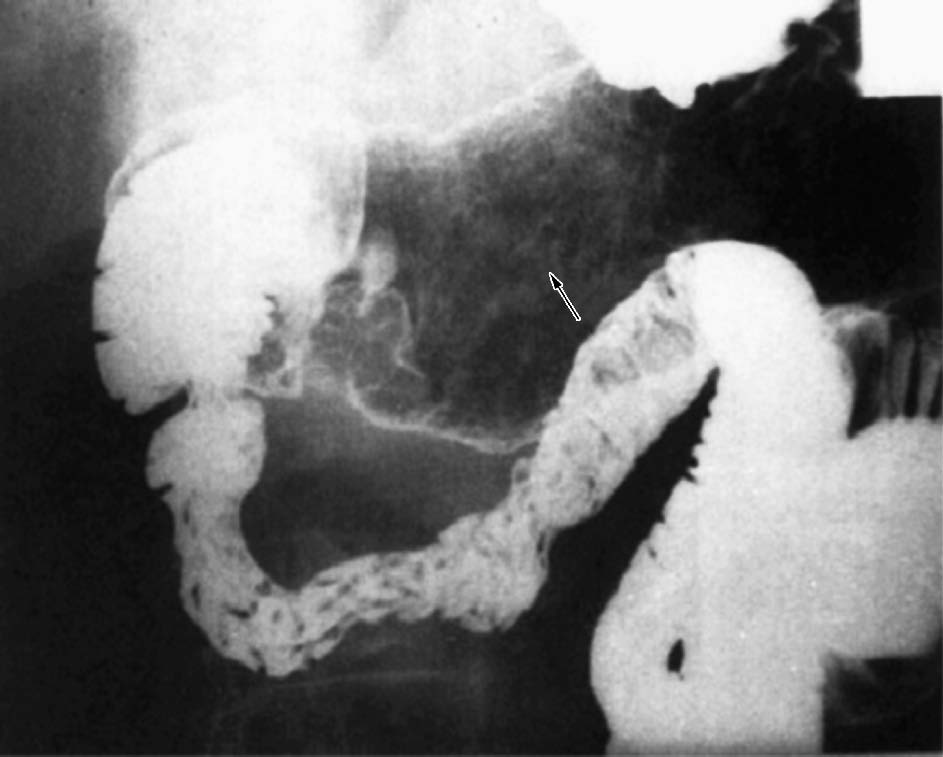
\includegraphics{./images/Image00278.jpg}
 \captionsetup{justification=centering}
 \caption{胃窦部早期胃癌(Ⅱa型)}
 \label{fig5-3-16}
  \end{figure} 

\textbf{【病史摘要】}
 女性,41岁。上腹部不适伴嗳气、反酸、食欲减退1个月。体格检查:腹软,上腹部轻度压痛,未扪及包块,心、肺阴性。

\textbf{【X线表现】}
 上消化道钡餐造影示:胃窦部见一形态不规则的平盘状充盈缺损影,表面凹凸不平,见小钡斑(箭头)。

\textbf{【X线诊断】}  胃窦部早期胃癌(Ⅱa型)。

\textbf{【评  述】}
 本例经手术病理证实为胃窦部早期胃癌Ⅱa型。胃双对比造影可显示粘膜面的细微结构而对早期胃癌的诊断具有重要价值。早期胃癌的X线表现主要为:①Ⅰ型(隆起型):肿瘤与周围粘膜有明显的分界,形态多不规则,呈息肉状、分叶状、菜花状等。表面不光滑,因有表层坏死形成粘膜缺损,双对比造影可见不规则钡斑。其基底部与正常粘膜分界清楚,侧面观可为广基型、无蒂型、有蒂型,有蒂者肿瘤在2cm以上。②Ⅱa型(表面隆起型):肿瘤形态不规则,呈平坦的息肉状、花坛状、平盘状等。表面有不规则凹凸而显示为不规则钡斑,基底部多为广基型。③Ⅱb型(表面平坦型):双对比造影主要表现为胃小区的细微变化,如胃小区粗大、紊乱,呈不规则之颗粒状形态。④Ⅱc型(表面凹陷型):肿瘤表现为形态不规则之表浅溃疡,呈楔形、星芒状等,边缘清楚、锐利,病变一般较小,病变周围伴有粘膜皱襞纠集现象,其粘膜皱襞尖端有明显的病理变形,如杵状增粗、笔尖样变细、阶梯状变薄、皱襞融合等。⑤Ⅲ型(凹陷型):为一深溃疡,其深溃疡本身不是癌,只于溃疡口边缘有癌浸润。X线表现其深溃疡形态很像良性溃疡,难以鉴别,只于溃疡口边缘显示轻微毛糙不平为其特征。由于早期胃癌的病变范围较小,因而X线双重造影检查的重点在于发现它的存在,最后的诊断需要密切结合内镜与活检方能明确。

\subsection{早期胃癌(Ⅱc型)}

\begin{figure}[!htbp]
 \centering
 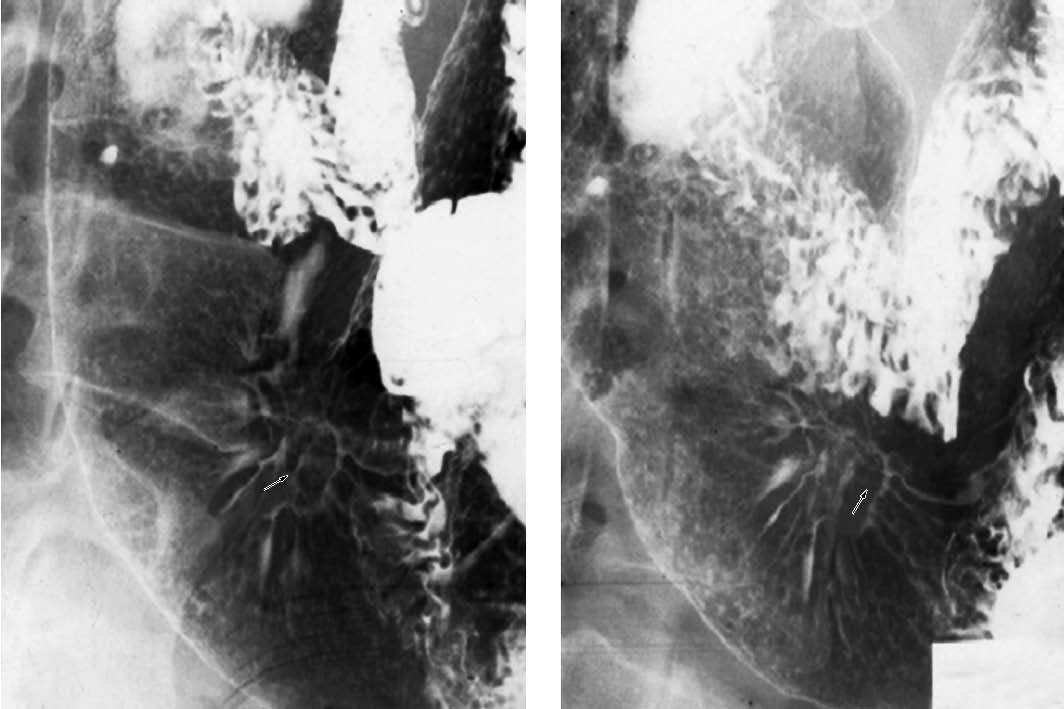
\includegraphics{./images/Image00279.jpg}
 \captionsetup{justification=centering}
 \caption{胃窦小弯侧早期胃癌(Ⅱc型)}
 \label{fig5-3-17}
  \end{figure} 

\textbf{【病史摘要】}
 男性,45岁。上腹部不适、疼痛3个月余,近1个月疼痛加重。体格检查:腹软,剑突下压痛,未扪及包块,心、肺阴性。

\textbf{【X线表现】}
 上消化道钡餐造影示:胃窦小弯侧见一小不规则钡斑,表面凹凸不平,周围粘膜皱襞纠集。

\textbf{【X线诊断】}  胃窦小弯侧早期胃癌(Ⅱc型)。

\textbf{【评  述】}
 本例经手术病理证实为胃窦部小弯侧粘膜下癌,未突破粘膜肌层。胃癌是我国最常见的恶性肿瘤之一,好发年龄为40~60岁,可发生在胃的任何部位,但以胃窦、胃小弯及贲门区常见。目前,国内外均采用日本内镜学会提出的早期胃癌的定义及分型。早期胃癌是指癌限于粘膜及粘膜下层,而不论其大小或有无转移。依据肉眼形态分为三个基本型与三个亚型:Ⅰ型,隆起型,癌肿隆起高度大于5mm,呈息肉状。Ⅱ型,浅表型,癌灶比较平坦,不形成明显隆起或凹陷。本型根据其癌灶凹凸程度不同又分三个亚型:Ⅱa型,浅表隆起型,癌灶隆起高度小于5mm。Ⅱb型,浅表平坦型,与周围粘膜几乎同高,无隆起或凹陷。Ⅱc型,浅表凹陷型,癌灶凹陷深度小于5mm。Ⅲ型,凹陷型,癌灶深度大于5mm,形成溃疡,癌组织不超过粘膜下层。除上述三型外,尚有混合型。根据胃窦小弯侧不规则形表浅凹陷形成边缘粗糙的钡斑,其周围粘膜皱襞纠集呈杵状增粗和融合,拟诊断为早期胃癌,浅表凹陷型(Ⅱc型)。需要鉴别的是良性溃疡病变,其钡斑密度均匀、边缘光整,多呈圆形、椭圆形,溃疡周围粘膜皱襞纠集一般比较均匀规则,呈自远而近逐渐变细,与癌可形成鲜明的对照。

\subsection{早期胃癌(Ⅱa+Ⅱc型)}

\begin{figure}[!htbp]
 \centering
 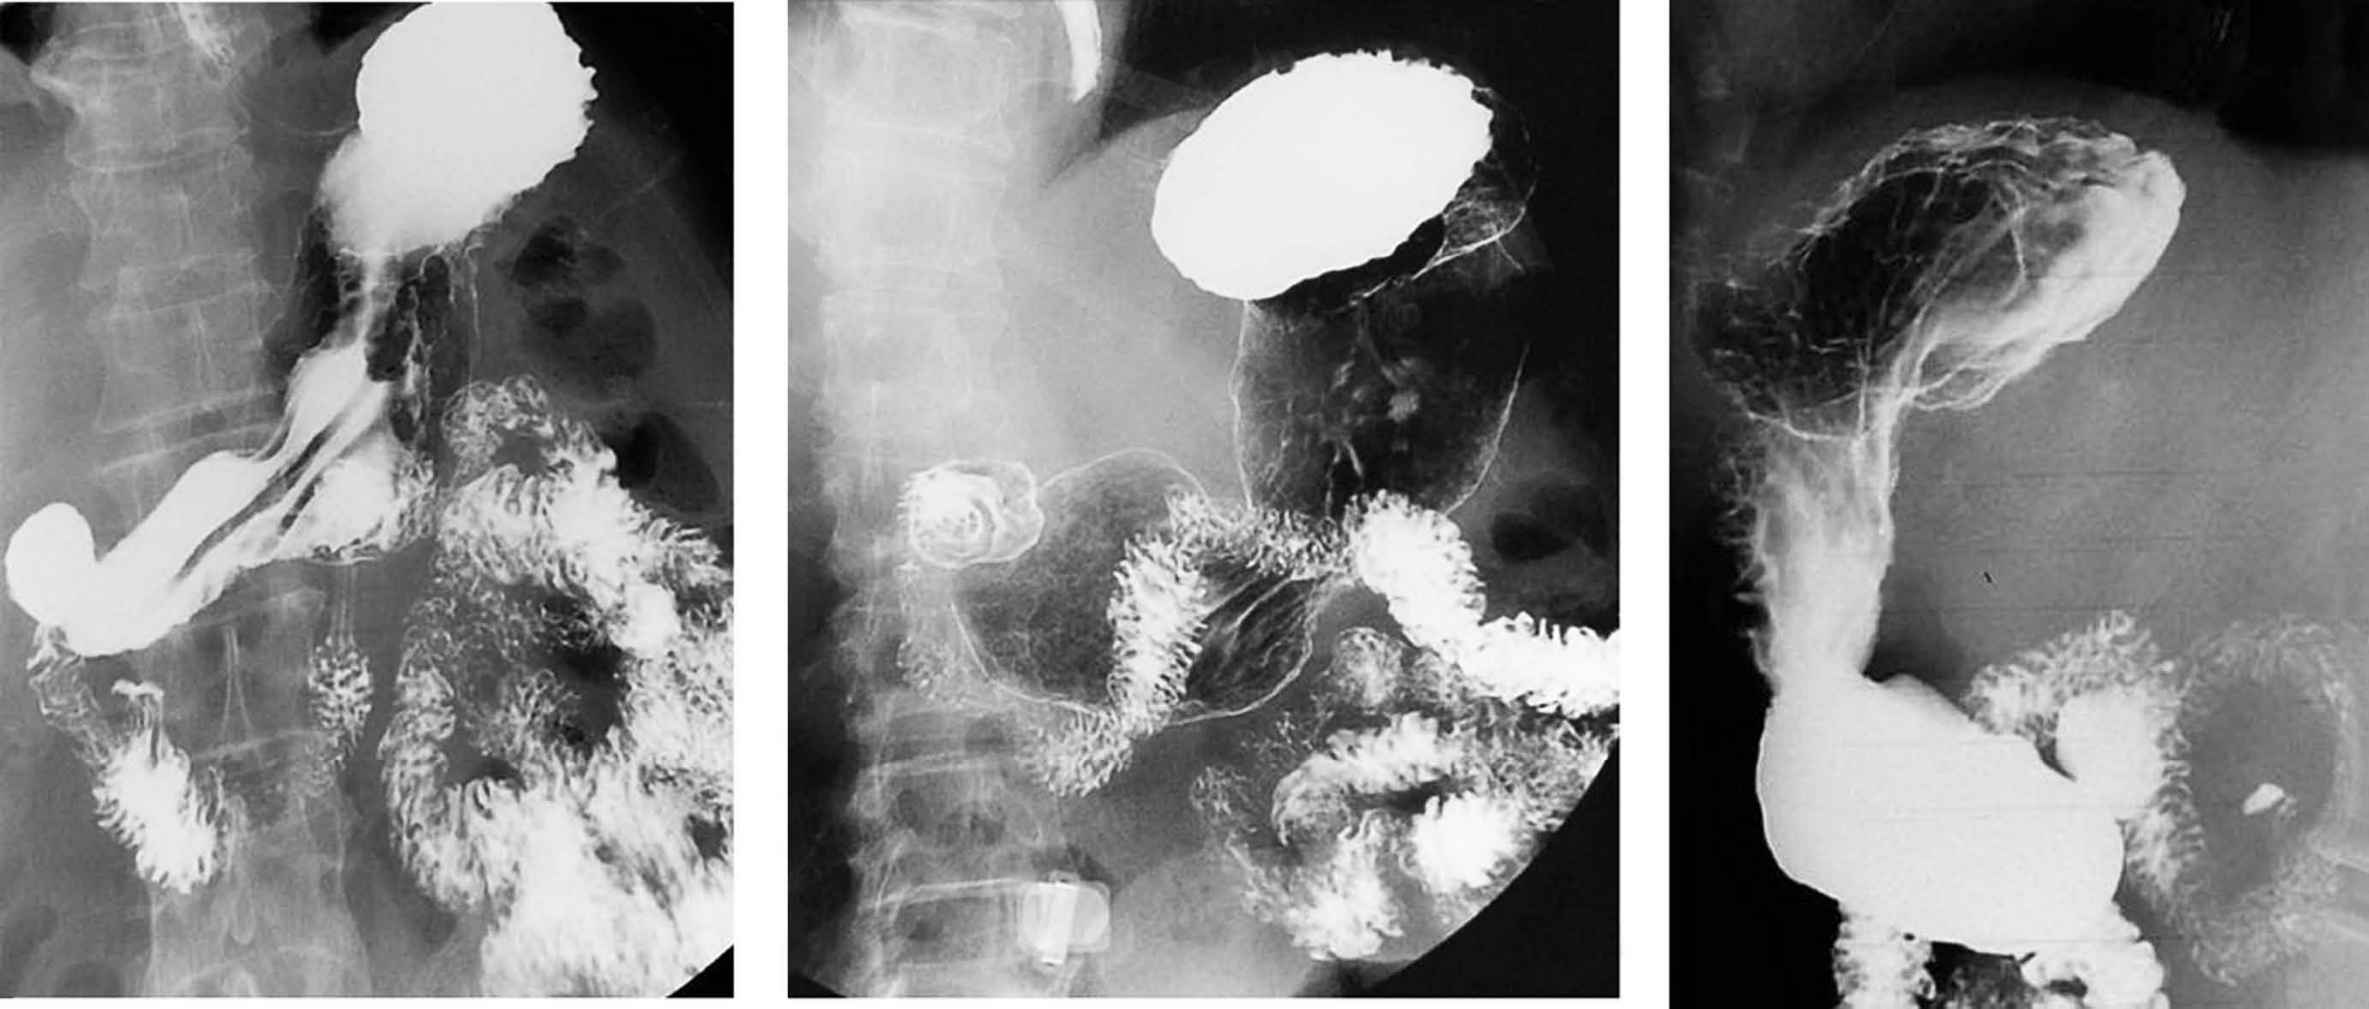
\includegraphics{./images/Image00280.jpg}
 \captionsetup{justification=centering}
 \caption{胃体部早期胃癌(Ⅱa+Ⅱc型)}
 \label{fig5-3-18}
  \end{figure} 

\textbf{【病史摘要】}
 女性,45岁。上腹部疼痛不适伴嗳气、反酸5个月,近1个月疼痛加重,食欲减退。体格检查:腹软,上腹部压痛,未扪及包块,心、肺阴性。

\textbf{【X线表现】}
 上消化道钡餐造影示:胃体上部见隆起型小充盈缺损影,边缘欠光整,表面凹凸不平,见不规则钡斑影,周围粘膜皱襞中断破坏,胃小弯侧上段胃壁僵硬。

\textbf{【X线诊断】}  胃体部早期胃癌(Ⅱa+Ⅱc型)。

\textbf{【评  述】}
 本例经手术病理证实为胃体上部早期胃腺癌(Ⅱa+Ⅱc型),粘膜肌层未侵犯,周围淋巴结未见转移。早期胃癌除上述三个基本型及亚型外,病灶若具有两种形态者,称之为混合型,一般表述时将占优势的一型记录在前,如本例为Ⅱa+Ⅱc型,表示隆起型病灶的中央存在糜烂的深凹陷。

\subsection{胃癌(息肉型)}

\begin{figure}[!htbp]
 \centering
 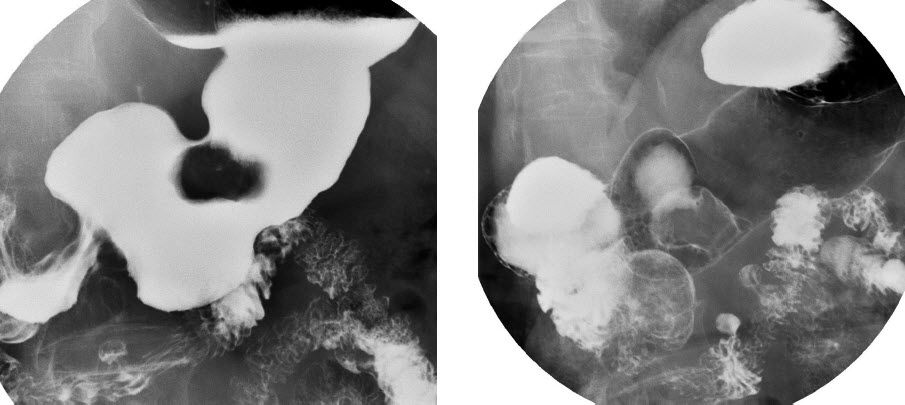
\includegraphics{./images/Image00281.jpg}
 \captionsetup{justification=centering}
 \caption{胃窦部胃癌(息肉型)}
 \label{fig5-3-19}
  \end{figure} 

\textbf{【病史摘要】}
 男性,52岁。上腹部疼痛2年,无节律性,近期疼痛加重。体格检查:上腹部压痛,未扪及明显包块,腹软,肝、脾未及,心、肺阴性。

\textbf{【X线表现】}
 上消化道钡餐造影示:胃窦部近小弯侧见一充盈缺损,呈分叶状,轮廓欠光整,周围粘膜皱襞中断破坏,局部胃壁较僵硬,十二指肠水平段见囊袋状影。

\textbf{【X线诊断】}  胃窦部胃癌(息肉型);十二指肠水平段憩室。

\textbf{【评  述】}
 本例患者经手术病理证实为胃体近小弯侧胃腺癌,侵犯胃粘膜肌层。息肉型胃癌为常见病,好发于胃窦部,其次是胃底。早期癌肿突向胃腔,高约5mm,轮廓大多不规则,可广基底或呈狭蒂。中后期,癌肿进一步增大,表面高低不平如菜花样,与胃壁边界明确。临床多见于40岁以上男性,早期无症状,或类似溃疡病的症状。中后期,症状加剧,有中上腹痛,上消化道出血,扪及肿块,以及癌肿所在部位所产生的一些继发症状,如梗阻、呕吐等。

X线特点主要为:早期隆起型胃癌在适当加压或双重造影检查时,可见小的轮廓不规则的充盈缺损。至中晚期,一般钡餐检查,即可显示出轮廓不光整的充盈缺损,基底广、边界明确、直径3~4cm以上。缺损区邻近粘膜纹中断、破坏,胃壁僵硬。早期隆起型胃癌主要应与胃内良性肿瘤相鉴别,胃癌充盈缺损边缘不光整,粘膜破坏,胃壁僵硬。中晚期胃癌应与胃内其他恶性肿瘤相鉴别。早期隆起型胃癌如果病灶较小,常规钡餐检查容易漏诊,应注意适当加压方能显示出病灶。内镜检查有利于发现早期病灶,并能提供病理依据,便于明确诊断。

\subsection{贲门癌}

\begin{figure}[!htbp]
 \centering
 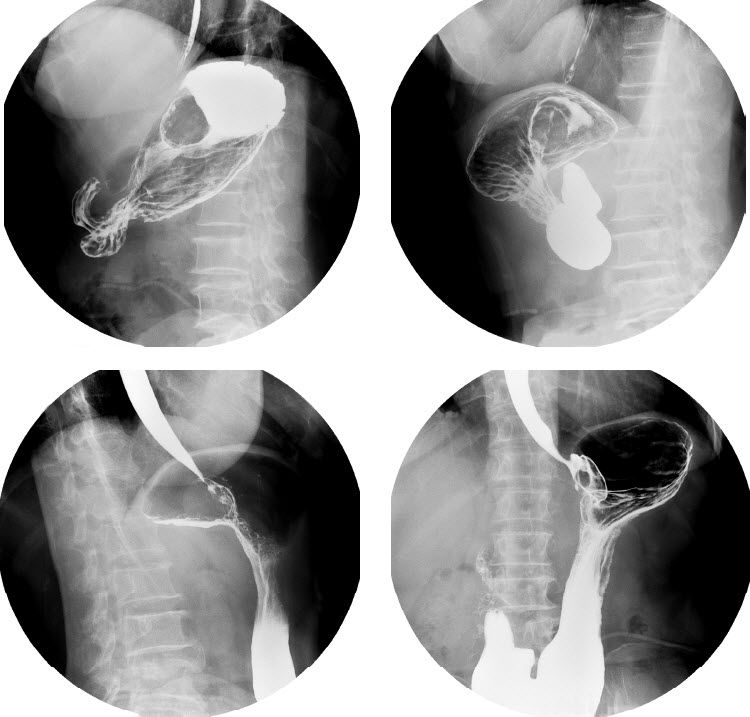
\includegraphics{./images/Image00282.jpg}
 \captionsetup{justification=centering}
 \caption{贲门癌}
 \label{fig5-3-20}
  \end{figure} 

\textbf{【病史摘要】}
 男性,56岁。上腹部疼痛、吞咽不适伴嗳气、反酸半年余,近1个月进食干性食物时吞咽困难加重伴呕吐。体格检查:腹软,上腹部轻度压痛,未扪及包块,心、肺阴性。

\textbf{【X线表现】}
 上消化道钡餐造影示:胃底贲门区见类圆形充盈缺损影,边缘毛糙,轻度分叶,周围粘膜皱襞破坏,胃体小弯侧上方胃壁僵硬。

\textbf{【X线诊断】}  贲门癌侵及胃体小弯上段(进展期)。

\textbf{【评  述】}
 本例患者经手术病理证实为胃底贲门腺癌,侵及胃体小弯侧上段。贲门癌为源于贲门中心周围2.0~2.5cm以内的胃癌。由于其位置比较特殊而易漏诊,主要原因为贲门区位于肋弓内不能触及肿块,贲门胃底部粘膜皱襞粗大使较小的病变难以识别。因此,检查贲门癌时应采用气钡双重造影,产气量越大越可形成良好的对比。一般先于立位观察,再采用仰卧、俯卧及左右斜位观察以免漏诊。

贲门癌的典型X线征象为:①贲门区肿物,可位于贲门开口上方或下方。②钡剂通过贲门时受阻,或在肿瘤之上绕过形成钡剂分流现象,有时呈喷射状入胃。③胃底增厚,呈多个弧形影,胃底与膈面距离加大(>1.5cm有诊断价值)。④贲门下方之胃小弯胃壁僵硬。⑤可合并龛影及出现环堤征。⑥食管下段受侵犯,出现狭窄、僵硬、变形等。

需要鉴别的是贲门失迟缓症,后者X线表现的食管下端狭窄对称、边缘光滑、壁柔软,管腔大小可变,腔内可见细而平行的粘膜皱襞,特别是无贲门癌胃泡内组织块影是鉴别要点。而发生于胃底的平滑肌瘤和平滑肌肉瘤,胃泡内也可见轮廓光整或分叶状软组织肿块影,但两者X线不仅有腔内的软组织肿块影,而且向胃腔外生长,还有胃壁改变,腔外较大肿块可推压邻近器官,再者平滑肌瘤与平滑肌肉瘤很少有侵犯食管下端,这些都与贲门癌不同。贲门区解剖结构特殊,发生于此的溃疡、静脉曲张及其他良恶性肿瘤X线表现与贲门癌有时差异也不显著,需密切结合临床病史,必要时做胃镜协助诊断。

\subsection{胃窦癌}

\begin{figure}[!htbp]
 \centering
 \includegraphics{./images/Image00283.jpg}
 \captionsetup{justification=centering}
 \caption{胃窦癌}
 \label{fig5-3-21}
  \end{figure} 

\textbf{【病史摘要】}
 女性,50岁。上腹部饱胀、疼痛2年,近2个月来疼痛加重,伴恶心、呕吐。体格检查:消瘦贫血貌,上腹部压痛并触及固定包块,心、肺阴性。

\textbf{【X线表现】}
 上消化道钡餐造影示:胃窦部狭窄,胃窦大弯侧见不规则充盈缺损,呈现肩胛征,胃窦部粘膜皱襞破坏紊乱,胃壁僵硬蠕动消失,胃内粘液潴留较多。

\textbf{【X线诊断】}  胃窦癌(进展期)。

\textbf{【评  述】}
 本例患者经手术病理证实为胃窦癌。胃窦部为胃癌另一好发部位,易发生浸润型胃癌,极易引起胃窦狭窄,狭窄的胃窦呈漏斗状或山峰状,出现肩胛征或袖口征,前者指狭窄的胃窦与其近端舒张的胃壁相连处呈肩胛状,后者则表现为狭窄近端随蠕动推进套在僵硬段上呈袖口状。此外,胃窦癌易于侵犯幽门而形成幽门梗阻,致胃排空延迟、胃残留物及滞留液增多,故必须做好检查前准备,清除和减少胃内滞留物。通常采用延长禁食时间和插胃管洗胃等方法,尚可使用辅助药物或针刺来改变胃窦张力和蠕动,以利于清晰显示狭窄段情况。胃窦癌须注意与胃窦炎或溃疡引起的良性狭窄相鉴别。鉴别的要点为良性狭窄病变段与正常胃分界呈渐进性,狭窄形态可变,可以收缩与扩张,粘膜皱襞存在、排列不整齐,其与胃窦癌形成的胃窦狭窄X线征象截然不同,鉴别不难。

\subsection{溃疡型胃癌}

\begin{figure}[!htbp]
 \centering
 \includegraphics{./images/Image00284.jpg}
 \captionsetup{justification=centering}
 \caption{胃小弯侧溃疡型胃癌}
 \label{fig5-3-22}
  \end{figure} 

\textbf{【病史摘要】}
 男性,65岁。上腹部疼痛不适2年,近1个月来疼痛加剧,消瘦明显。体格检查:消耗面容,上腹部可触及固定硬质包块,压痛明显,心、肺阴性。

\textbf{【X线表现】}
 上消化道钡餐造影示:胃角处胃腔内见一不规则龛影,龛影周围显示有不规则透亮环堤,其内可见指压迹征和裂隙征,局部胃壁僵硬,蠕动消失。

\textbf{【X线诊断】}  胃小弯侧溃疡型胃癌(进展期)。

\textbf{【评  述】}
 本例患者经手术后病理证实为胃小弯侧腺癌。溃疡型胃癌是进展期胃癌中的最多见类型,其X线表现以壁龛及邻近胃壁变化为主要表现。龛影多数较浅而大,形态多不规则,具有特征性的为口部指压迹征和裂隙征,与良性溃疡平坦的口部出现的狭颈征、项圈征对比分明。切线位显示龛影位于胃轮廓线以内或与之相平。龛影周围一圈不规则充盈缺损为环堤,环堤大小不一,高低不平,与正常胃壁界限清楚,其病理基础为癌肿破溃后留下的一圈隆起的边缘。若龛影骑跨于胃小弯前后壁,与周围的半弧形环堤构成了半月综合征。邻近粘膜皱襞亦可有聚拢表现,但近环堤处粘膜中断且有指压迹改变。

\subsection{浸润型胃癌}

\begin{figure}[!htbp]
 \centering
 \includegraphics{./images/Image00285.jpg}
 \captionsetup{justification=centering}
 \caption{浸润型胃癌}
 \label{fig5-3-23}
  \end{figure} 

\textbf{【病史摘要】}
 女性,48岁。上腹部疼痛2年,嗳气、反酸,近1个月来疼痛加剧,出现黑便,食欲减退。体格检查:消瘦,肝、脾未及,腹壁紧张,全腹压痛,心、肺阴性。

\textbf{【X线表现】}
 上消化道钡餐造影示:全胃胃腔缩小,胃壁僵硬,无蠕动,粘膜皱襞增粗、紊乱,呈脑回状改变,形态固定不变。

\textbf{【X线诊断】}  广泛浸润型胃癌(皮革胃)。

\textbf{【评  述】}
 本例患者经手术病理证实为高度恶性晚期进展期胃癌,X线表现呈皮革状胃,癌肿全胃广泛浸润。浸润型胃癌根据癌肿浸润范围不同,X线表现可分为局限浸润型和弥漫浸润型。局限型可发生于胃的任何部位,以胃窦部多见。X线表现为:癌肿浸润胃壁全周或半周时,胃腔显示为局限性、固定性狭窄与僵硬,严重时可呈管状、漏斗状狭窄。胃壁局限性僵硬、蠕动消失。胃粘膜皱襞增粗、紊乱,部分呈脑回状,形态固定不变。广泛型为癌肿浸润胃大部或全部,胃腔明显缩小,粘膜皱襞平坦、消失,胃壁僵硬、蠕动消失,犹如皮革囊状,称皮革胃。因幽门受侵而失去正常功能,由于钡剂的重力作用,可见造影时幽门处于开放状态,有造影剂源源不断地进入十二指肠。浸润型胃癌有时应和胃淋巴瘤相鉴别。胃淋巴瘤主要为粘膜下浸润性生长,肌层较少受浸润,且又无明显的纤维组织增生,故胃壁虽可增厚,但胃腔缩小一般不明显,胃壁僵硬也不显著,往往可见有蠕动波为鉴别之要点。

\subsection{残胃癌}

\begin{figure}[!htbp]
 \centering
 \includegraphics{./images/Image00286.jpg}
 \captionsetup{justification=centering}
 \caption{残胃癌}
 \label{fig5-3-24}
  \end{figure} 

\textbf{【病史摘要】}
 男性,65岁。5年前因溃疡型胃癌行胃大部分切除术、Billroth
Ⅰ式吻合术,近期上腹部疼痛加重伴嗳气、反酸,并有恶心、呕吐。体格检查:消瘦,皮肤、巩膜无黄染,左上腹部压痛明显,肝、脾无增大,心、肺阴性。

\textbf{【X线表现】}
 上消化道钡餐造影示:残胃吻合口下部小弯侧见不规则龛影,龛影周围显示有不规则透亮环堤,其内可见指压迹征,局部胃壁僵硬,蠕动消失。

\textbf{【X线诊断】}  残胃癌。

\textbf{【评  述】}
 本例患者经手术病理证实为残胃癌。残胃癌的诊断标准不一,国外多主张因良性疾患行胃部分切除术、胃肠吻合术后3年以上,残胃生癌者为残胃癌。我国主张良性胃疾患胃部分切除术后3年以上,胃癌行部分切除术后5年以上,残胃生癌者称残胃癌。国内外材料一致认为,胃空肠吻合术后残胃癌发生率高于胃十二指肠吻合术者。残胃癌病因不明,可能与碱性肠液刺激及术后引起吻合口慢性刺激有关。早期残胃癌临床症状不具特征性。中晚期残胃癌常见症状是中上腹疼痛、食欲减退和出血。残胃癌好发于胃残端部,其次为贲门区和大小弯前后壁交界部。因术后粘连及变形,残胃癌的X线诊断困难。常见的表现为吻合口狭窄、排空迟缓、残胃扩张;胃腔狭窄变形,胃壁僵直丧失舒缩功能;粘膜破坏;充盈缺损或不规则龛影等。残胃癌应与炎症性粘膜肿胀、缝线引起的异物反应或肉芽肿等鉴别,手术缝合时,可使小弯侧结节状改变也应注意,鉴别困难时,应结合纤维胃镜检查及组织学检查。

\section{十二指肠病变}

\subsection{十二指肠球部溃疡}

\begin{figure}[!htbp]
 \centering
 \includegraphics{./images/Image00287.jpg}
 \captionsetup{justification=centering}
 \caption{十二指肠球部溃疡}
 \label{fig5-4-1}
  \end{figure} 

\textbf{【病史摘要】}
 男性,55岁。上腹部节律性疼痛伴反酸2年,餐后疼痛缓解。体格检查:上腹部剑突下压痛,肝、脾无肿大,心、肺阴性。

\textbf{【X线表现】}
 上消化道钡餐造影示:十二指肠球基底部见一龛影,黄豆大小,边缘光整,周围粘膜纠集,球部变形。

\textbf{【X线诊断】}  十二指肠球部溃疡。

\textbf{【评  述】}
 本例经胃镜证实为十二指肠球部溃疡。十二指肠溃疡为常见病,其发生率高于胃溃疡。十二指肠溃疡好发于青壮年,40岁以下占80%。男性多于女性。十二指肠溃疡病因复杂,尚未完全阐明。十二指肠溃疡85%发生于球部,其次在球后部。发生于球部者,前壁较多,占50%,其次为后壁及球部的大小弯。单发为主,也可多发。临床主要征象为周期性、节律性右上腹痛,多在餐后3~4小时发生,进餐后可缓解。

X线表现主要有:①球部龛影,为球部溃疡的直接征象,正面观呈圆形或椭圆形,少数呈线状,需双重造影显示。充盈加压时,溃疡周围的水肿、增生表现为外缘模糊的透光带。切线位上龛影突出于轮廓线以外,呈锥形或乳头状,以充盈像显示较好。②球部变形,多由溃疡所致,少数可因胆系或胰腺等邻近脏器疾病所致,因此发现球部变形时需除外其他原因后方可诊断溃疡。球部呈二叶状、山字形、花瓣状畸形为瘢痕收缩的结果,球部的大、小弯侧可见袋状突出,称假性憩室,也因瘢痕收缩所致。球部整体性痉挛及严重的瘢痕收缩皆可致明显缩窄,此时常伴幽门梗阻,平滑肌松弛剂的应用有助于痉挛与瘢痕挛缩的鉴别。③激惹征,表现为钡剂迅速经过球部而不能满意充盈,为炎症刺激所致。

\subsection{十二指肠复合性溃疡}

\begin{figure}[!htbp]
 \centering
 \includegraphics{./images/Image00288.jpg}
 \captionsetup{justification=centering}
 \caption{十二指肠复合性溃疡}
 \label{fig5-4-2}
  \end{figure} 

\textbf{【病史摘要】}
 男性,35岁。上腹部不适、嗳气、反酸1年,近日夜间疼痛加重,饥饿时加重,进食后缓解。体格检查:上腹部剑突下压痛,肝、脾无增大,心、肺阴性。

\textbf{【X线表现】}
 上消化道钡餐造影示:十二指肠球部及球后部见大小不等龛影,球部变形呈二叶形,十二指肠上曲狭窄,钡剂下行受阻。

\textbf{【X线诊断】}  十二指肠复合性溃疡。

\textbf{【评  述】}
 本例患者经胃镜检查证实为十二指肠复合性溃疡,即十二指肠球部及球后部溃疡。十二指肠球后部是指球部与降部之间的肠管。该部溃疡以龛影为主,可合并局限性偏心性狭窄,十二指肠激惹征较为明显,局部压痛可同时存在。由于球部的重叠,十二指肠球后部溃疡较难显示。检查的方法包括以下三方面:①常规钡餐,利用各种体位及结合加压来显示病变,可以较好地了解球部充盈及排空情况以及十二指肠蠕动状况。②低张气钡造影,能更清晰地显示细微结构及病变情况。③内镜应用,钡餐结合内镜所见来提高诊断率已经成为一种必不可少的手段。

\subsection{肠系膜上动脉压迫综合征}

\begin{figure}[!htbp]
 \centering
 \includegraphics{./images/Image00289.jpg}
 \captionsetup{justification=centering}
 \caption{肠系膜上动脉压迫综合征}
 \label{fig5-4-3}
  \end{figure} 

\textbf{【病史摘要】}
 女性,35岁。进食后上腹部饱胀恶心、呕吐,俯卧位后症状缓解。体格检查:瘦长体形,肝、脾未及,腹部无明显压痛,心、肺阴性。

\textbf{【X线表现】}
 上消化道钡餐造影示:无力型胃,胃角位于髂嵴连线下方2.5cm左右,蠕动缓慢。十二指肠水平段钡剂受阻,水平段以上肠管扩张,蠕动亢进,并见逆蠕动发生,受阻处十二指肠见管状压迹。

\textbf{【X线诊断】}  肠系膜上动脉压迫综合征;胃下垂。

\textbf{【评  述】}
 本例患者经腹部CT扫描及CTA检查,示肠系膜上动脉自腹主动脉分出后,夹角过小,压迫十二指肠水平段,引起十二指肠郁积,故确诊为肠系膜上动脉压迫综合征。肠系膜上动脉压迫综合征多见于中年体弱和瘦长体形者,女性多于男性。其主要原因为肠系膜上动脉根部紧张度增强或先天性原因使肠系膜上动脉与腹主动脉间夹角变小,引起十二指肠水平段受压,使受压部以上肠管扩张而出现郁积。临床上主要表现为食后上腹部饱胀、恶心、呕吐,且呕吐物中带有胆汁,俯卧位时症状缓解或消失。X线表现主要是立位检查时钡剂通过十二指肠水平段受阻,十二指肠降段以上肠管扩张,蠕动亢进,可见钡剂如钟摆样来回运动,水平段受压处有一光滑整齐的纵形压迹,称为笔杆状压迹,使肠管紧贴脊柱,粘膜变平,当患者俯卧位时,该压迹可消失。诊断本病时应谨慎,因正常瘦长体形的人也可出现十二指肠水平段钡剂暂时性停留和少量逆蠕动,但无肠管扩张及胃排空延迟。此外,还需与器质性病变所致的梗阻相鉴别,若梗阻端形态显示良好,鉴别应无困难。

\subsection{十二指肠憩室}

\begin{figure}[!htbp]
 \centering
 \includegraphics{./images/Image00290.jpg}
 \captionsetup{justification=centering}
 \caption{十二指肠降部憩室}
 \label{fig5-4-4}
  \end{figure} 

\textbf{【病史摘要】}
 男性,45岁。上腹部疼痛不适月余。体格检查:上腹部剑突下压痛,肝、脾无增大,心、肺阴性。

\textbf{【X线表现】}
 上消化道钡餐造影示:胃窦部粘膜皱襞增粗、紊乱,胃壁柔软,十二指肠降部见一囊袋状影突出于肠壁,内见钡剂充盈,可见十二指肠粘膜纹理伸入其中。

\textbf{【X线诊断】}  胃窦炎;十二指肠降部憩室。

\textbf{【评  述】}
 本病比较常见,大多数患者无明显症状,多见于中老年人。发生部位多位于降段内后壁,其次为十二指肠水平段。若合并憩室炎可引起糜烂、溃疡和出血,壶腹部附近憩室尚可引起胆管炎或胰腺炎等。十二指肠憩室发生的原因可能与肠壁生长发育过程中的局部缺陷与薄弱有关,随着年龄增长而加剧退变,在肠内压异常增加或肠肌收缩不协调时,薄弱点向腔外突出而形成憩室。十二指肠憩室X线表现主要是充钡后憩室呈圆形、椭圆形或三角形囊袋状突出物,轮廓光整,颈部较狭窄,并可见十二指肠粘膜皱襞伸入其中。憩室大小不一,较大者立位可见囊内气、液、钡分层现象,较小者可呈短管状,一般钡透不易发现,需行低张气钡双重造影才不至于漏诊。憩室轮廓不规则、压痛、邻近十二指肠有肠激惹征象者应考虑合并憩室炎。此外,憩室尚需与溃疡鉴别,后者常伴有狭窄痉挛,龛影内无粘膜皱襞伸入。

\subsection{十二指肠腺瘤}

\begin{figure}[!htbp]
 \centering
 \includegraphics{./images/Image00291.jpg}
 \captionsetup{justification=centering}
 \caption{十二指肠腺瘤}
 \label{fig5-4-5}
  \end{figure} 

\textbf{【病史摘要】}
 男性,45岁。上腹部疼痛不适,有嗳气、反酸。体格检查:上腹部剑突下压痛,肝、脾无增大,心、肺阴性。

\textbf{【X线表现】}
 上消化道钡餐造影示:十二指肠降部下段外侧可见分叶状充盈缺损(箭头),其基底部与肠壁形成切迹,肠壁略凹陷,周围粘膜皱襞正常,未见明显中断、破坏。

\textbf{【X线诊断】}  十二指肠降部腺瘤。

\textbf{【评  述】}
 本例经手术病理证实为十二指肠降部腺瘤。十二指肠良性肿瘤约占小肠良性肿瘤的20%。以腺瘤、平滑肌瘤、脂肪瘤多见。发生部位以球部最多,占50%以上,降部次之,升部最少。肿瘤多向肠腔内呈息肉状生长,少数向肠腔外生长。临床上多见于老年人,因肿瘤多较小而少有症状。食欲不振、恶心、上腹部疼痛及出血为常见症状。十二指肠腺瘤与消化道其他部位的腺瘤相似,X线表现为圆形、椭圆形或分叶状充盈缺损,边缘光滑,局部肠壁柔软,粘膜皱襞无破坏,一般以单发为多见,少数可多发,可带蒂,此时可见肿瘤随肠蠕动而移动。腺瘤多发时要与布氏腺增生鉴别。布氏腺增生比较罕见,多发生在球部,亦可延及降部。病因不明,通常认为是一种炎症。病理上有多发型和单发型两种,前者为广泛结节状粘膜增生,后者与单发腺瘤相似,可带蒂。X线表现为十二指肠球部粘膜紊乱,皱襞增粗,其中可见多枚黄豆或绿豆大小的充盈缺损,形态固定。单发者为单个充盈缺损,与腺瘤无法鉴别,通常十二指肠没有激惹和变形。

一般临床工作中,如发现十二指肠单发带蒂肿瘤应首先考虑腺瘤的诊断,而十二指肠多发结节状充盈缺损则应首先考虑布氏腺增生的诊断。最终诊断要结合内镜或手术病理诊断。

\subsection{十二指肠平滑肌瘤}

\begin{figure}[!htbp]
 \centering
 \includegraphics{./images/Image00292.jpg}
 \captionsetup{justification=centering}
 \caption{十二指肠平滑肌瘤}
 \label{fig5-4-6}
  \end{figure} 

\textbf{【病史摘要】}
 男性,35岁。上腹部疼痛不适月余,无嗳气、反酸,无恶心、呕吐。体格检查:上腹部无压痛,肝、脾无增大,心、肺阴性。

\textbf{【X线表现】}
 上消化道钡餐造影示:十二指肠下曲见类圆形充盈缺损影,边缘光整,内见小钡斑影,十二指肠腔未见狭窄,肠壁未见僵硬,蠕动正常。

\textbf{【X线诊断】}  十二指肠平滑肌瘤。

\textbf{【评  述】}
 本例患者经手术治疗病理证实为十二指肠平滑肌瘤。本例患者十二指肠病变X线征象符合良性肿瘤的表现,发生于十二指肠的良性肿瘤较少见,以平滑肌瘤及腺瘤多见。平滑肌瘤来源于中胚层组织。

X线表现主要为:①小肠局限性肿物,瘤体一般<5cm。②肿物呈球形或分叶状,周界规则,切线位上呈半圆形充盈缺损。③向腔内生长者,肿瘤一般体积都较大,无蒂,较固定,活动度差,局部管腔狭窄,可致肠梗阻;腔外生长者多无临床症状;如同时向腔内及腔外生长,尚可见肠管受压甚至移位。④瘤体中心因血供缺乏,往往容易发生坏死,出现龛影或表面糜烂,X线表现为钡斑。需要指出的是,平滑肌瘤和平滑肌肉瘤皆为粘膜下肿瘤,均具有粘膜下肿瘤的特征,故两者X线表现有时很相似,鉴别有一定难度。但平滑肌肉瘤瘤体体积常大于5cm,形态不规则,表面常凹凸不平,并且常较早出现肝脏、淋巴结转移,这有利于两者的鉴别诊断。

\subsection{十二指肠腺癌}

\begin{figure}[!htbp]
 \centering
 \includegraphics{./images/Image00293.jpg}
 \captionsetup{justification=centering}
 \caption{十二指肠降部腺癌}
 \label{fig5-4-7}
  \end{figure} 

\textbf{【病史摘要】}
 男性,65岁。上腹部疼痛不适伴呕吐3个月余,近期有黑便。体格检查:腹软,中上腹部压痛,肠肠鸣音正常,肝、脾未及,心、肺阴性。

\textbf{【X线表现】}
 上消化道钡餐造影示:十二指肠降部管腔明显环形狭窄,粘膜破坏,管壁僵硬,蠕动消失,近端肠管扩张。

\textbf{【X线诊断】}  十二指肠降部腺癌。

\textbf{【评  述】}
 本例经手术治疗病理证实为十二指肠降部粘液腺癌。十二指肠腺癌占小肠腺癌的40%~50%,好发于60~70岁,男女之比约为1.2∶1。按癌瘤发生的部位可分为乳头上部癌、乳头周围癌和乳头下部癌,其中以乳头周围癌最多见,约占65%,乳头上部癌约占20%,乳头下部癌约占15%。按肿瘤的大体形态可分为息肉型、浸润溃疡型、缩窄型和弥漫型。临床表现与肿瘤的类型及部位有关。主要症状有:上腹部隐痛、烧灼样痛或钝痛:酷似十二指肠溃疡,但进食及制酸药均不能缓解疼痛。黄疸:乳头周围癌75%~80%可发生黄疸。肠梗阻:息肉型或缩窄型癌容易导致肠腔狭窄或堵塞,导致部分或完全性十二指肠梗阻;乳头上部癌导致的完全性肠梗阻,呕吐物内不含胆汁,易被误诊为幽门梗阻。出血:十二指肠癌患者的大便隐血试验阳性者占60%~80%,出血明显者可有黑便,大出血时可发生呕血。腹块:右上腹出现肿块者占10%~25%。

根据肿瘤的X线表现可分为息肉型、溃疡型及浸润型:①息肉型:表现为息肉样隆起病变,形态不规则呈分叶状,粘膜破坏消失。肠腔可呈扩张状,钡剂分流,如果肿块较大可填塞十二指肠,钡剂受阻,近端肠腔扩张。同时也可伴有溃疡,肠壁僵硬等。②溃疡型:表现为粘膜破坏,出现不规则的腔内龛影,或部分腔内部分位于腔外。溃疡口部可有环堤、裂隙征及指压痕等恶性溃疡的征象。同时也可伴有局部肠壁僵硬,出现不规则的隆起性改变。③浸润型:X线表现为肠壁受到肿瘤浸润而僵硬,蠕动消失,肠腔狭窄,近端肠腔扩张,粘膜破坏,可伴有溃疡及不规则隆起性病变。本例患者为发生在十二指肠乳头上部的浸润型腺癌,X线表现比较明确,手术病理予以证实。但十二指肠癌如发生在乳头区则需与胰头癌相鉴别。十二指肠癌可推移相对正常的胰头或钓突结构向前内侧移位,肿块密度不均匀伴溃疡形成,十二指肠内外侧壁都呈不规则增厚和肠腔狭窄等有助于与胰头癌鉴别。但当肿瘤侵犯胰头时,两者的鉴别极为困难。

\subsection{十二指肠平滑肌肉瘤}

\begin{figure}[!htbp]
 \centering
 \includegraphics{./images/Image00294.jpg}
 \captionsetup{justification=centering}
 \caption{十二指肠平滑肌肉瘤}
 \label{fig5-4-8}
  \end{figure} 

\textbf{【病史摘要】}
 男性,55岁。上腹部疼痛半年余,无嗳气、反酸,无明显节律性。近期疼痛突然加剧,伴恶心、呕吐。体格检查:腹部拒按,上腹部触及包块,肝、脾未及,心、肺阴性。

\textbf{【X线表现】}
 上消化道钡餐造影示:十二指肠肠曲扩大,上曲内缘呈弧形压迹,肠腔伴有狭窄,其边缘皱襞有不规则破坏,并可见一不规则线状钡影呈水平状伸向十二指肠肠曲内,其上方见一小憩室。

\textbf{【X线诊断】}  十二指肠降部平滑肌肉瘤,肿瘤液化坏死与肠腔相通。

\textbf{【评  述】}
 本例患者经手术治疗病理证实为十二指肠降部平滑肌肉瘤,肿瘤液化坏死与肠腔相同。平滑肌肉瘤发生于十二指肠较少见。其病理变化与肿瘤生长方式有关,如肿瘤向肠腔内生长,呈半球状突入肠腔,可略有分叶,广基底,粘膜面糜烂或呈不规则溃疡,如肿瘤向肠腔外生长,则压迫十二指肠移位。临床可扪及腹块,质硬;可伴上消化道出血。

X线表现主要有:①腔内充盈缺损,略带有分叶改变,局部粘膜纹消失,可伴有不规则龛影,肠腔扩张,钡流改道。②肠腔被压迫移位,导致十二指肠肠曲变形,其形态改变依据肿瘤的部位和大小而定。上述两方面变化,有时混合存在。平滑肌瘤和平滑肌肉瘤皆为粘膜下肿瘤,均具有粘膜下肿瘤的特征,故两者X线表现有时很相似,鉴别有一定难度。但本例患者瘤体体积较大,形态不规则,表面凹凸不平,肿瘤液化坏死,并出现与肠腔相通的窦道,肠壁较僵硬,局部蠕动消失,与平滑肌瘤的表现相异,故诊断为平滑肌肉瘤。

\subsection{十二指肠淋巴瘤}

\begin{figure}[!htbp]
 \centering
 \includegraphics{./images/Image00295.jpg}
 \captionsetup{justification=centering}
 \caption{十二指肠淋巴瘤}
 \label{fig5-4-9}
  \end{figure} 

\textbf{【病史摘要】}
 男性,40岁。上腹部疼痛不适伴低热,无嗳气、反酸,偶有呕吐。体格检查:上中腹部压痛,中腹部似触及包块,肝、脾未及,心、肺阴性。

\textbf{【X线表现】}
 上消化道钡餐造影示:十二指肠降部中上段(箭头)肠腔狭窄,见不规则充盈缺损及小龛影,粘膜中断,肠壁略显僵硬。

\textbf{【X线诊断】}  十二指肠降部淋巴瘤。

\textbf{【评  述】}
 本例患者经内镜检查并经病理证实为十二指肠降部非霍奇金淋巴瘤。原发性十二指肠恶性淋巴瘤(primary
malignant lymphoma of
duodenum),是指原发于十二指肠肠壁淋巴组织的恶性肿瘤,原发性十二指肠恶性淋巴瘤好发于40岁左右,较其他恶性肿瘤发病年龄轻,男女发病之比为1:1~3:1。该病的临床表现无特异性,可因肿瘤的类型和部位而异,主要表现为上腹痛、腹块、弛张热等。病理巨检表现有浸润型、息肉型、溃疡型,可混合存在。

X线平片检查有时可显示十二指肠梗阻的X线表现,或软组织块影。胃肠道钡餐双重对比造影对十二指肠肿瘤的诊断准确率达42%~75%,其影像表现有:①十二指肠粘膜皱襞变形、破坏、消失,肠壁稍僵硬。②肠壁充盈缺损、龛影或环状狭窄。③肠管可有局限性囊样扩张,呈动脉瘤样改变。④肠壁增厚,肠管变小,呈多发性结节状狭窄。十二指肠低张造影,更有利于观察粘膜皱襞的细微改变,使其诊断准确率提高到93%左右。肠穿孔是本病的主要并发症,有15%~20%的十二指肠恶性淋巴瘤患者会发生肠穿孔,比其他恶性肿瘤发生率高。此多为肿瘤侵犯肠壁发生溃疡、肠坏死,或肿瘤继发感染而引致。本例患者十二指肠降部肠腔狭窄,肠壁见充盈缺损,内见小龛影,周围粘膜皱襞破坏,肠壁略显僵硬,故符合十二指肠淋巴瘤的诊断,最终需经内镜检查或手术行活检以获病理确诊。

\subsection{十二指肠类癌}

\begin{figure}[!htbp]
 \centering
 \includegraphics{./images/Image00296.jpg}
 \captionsetup{justification=centering}
 \caption{十二指肠类癌}
 \label{fig5-4-10}
  \end{figure} 

\textbf{【病史摘要】}
 男性,39岁。上腹部疼痛不适3个月余,无恶心、呕吐。体格检查:腹软,中腹部压痛,未触及包块,肝、脾未及,心、肺阴性。

\textbf{【X线表现】}
 上消化道钡餐造影示:十二指肠降部及水平部见不规则充盈缺损,局部粘膜破坏,肠壁稍僵硬,肠腔稍窄。

\textbf{【X线诊断】}  十二指肠占位:淋巴瘤?腺癌?类癌?

\textbf{【评  述】}
 本例患者经手术病理证实为十二指肠降部恶性神经内分泌癌,即类癌。十二指肠类癌是很特殊的一种类癌,好发部位依次为十二指肠第二段、第一段、第三段。年龄22~84岁,平均55岁。男女发病率差别不大。常合并Von
Recklinghausen's病、Zollinger-Ellison综合征和多发性内分泌肿瘤(MEN)。十二指肠和壶腹部还可发生杯状细胞类癌(腺类癌)和小细胞神经内分泌癌。杯状细胞类癌又称腺类癌或粘液类癌。主要病理改变为息肉状病变,大小不等,单发或多发,小的表现为粘膜下结节,大的则明显突向腔内,以致肠腔阻塞。局部常伴有腔外肿块。可合并有其他小肠、结肠或肺、气管类癌。临床症状无特征性,可扪及腹块。

类癌瘤较小时常被漏诊,发展到一定大小后,X线即可表现为:①病变范围内大小不等的结节状透亮区,或较大的充盈缺损,缺损区伴有肠腔外肿块,为本病重要表现之一。②病变区粘膜纹粗大,可伴有肠腔狭窄。③病变段肠曲固定,移动度消失。④病变可多发,同时可见于胃肠道的其他部分,甚至肺、支气管,亦有类癌瘤存在。类癌的鉴别诊断极为困难,因其表现多样化,仅凭影像学表现很难与其他肠道的良恶性肿瘤鉴别。以往主要依赖消化道钡剂造影,病变检出的阳性率较低。但CT广泛使用后,尤其是多层螺旋CT的使用大大提高了肿瘤的发现比例。CT不但可发现原发病灶,还可显示肿瘤对邻近组织的侵犯情况,观察肝脏的转移灶,肠系膜的侵犯,后腹膜及邻近淋巴结的转移。

\section{小肠病变}

\subsection{空肠憩室}

\begin{figure}[!htbp]
 \centering
 \includegraphics{./images/Image00297.jpg}
 \captionsetup{justification=centering}
 \caption{空肠憩室}
 \label{fig5-5-1}
  \end{figure} 

\textbf{【病史摘要】}
 男性,45岁。上腹部疼痛半年余伴腹胀。体格检查:腹软,腹部无明显压痛,未扪及包块,肝、脾未及,心、肺阴性。

\textbf{【X线表现】}
 全消化道钡餐造影示:空肠见一卵圆形袋状阴影,边缘整齐光滑,以宽窄不等的开口通向肠腔,内见钡剂进出。

\textbf{【X线诊断】}  空肠憩室。

\textbf{【评  述】}
 憩室是由于钡剂经过胃肠道管壁的薄弱区向外膨出形成的囊袋状影像,或是由于管腔外邻近组织病变的粘连、牵拉造成管壁全层向外突出的囊袋状影像,其内及附近的粘膜皱襞形态正常,称之为憩室。小肠憩室好发于上段空肠,少数在回肠。正常空肠上段的终末血管粗大,肠系膜缘血管进入处的肠壁结构较薄弱,容易成为憩室的好发部位。憩室可为单发,多为多发性,多个憩室集中于某段空肠。多发性憩室数目由2~40个不等;直径由数毫米到数厘米。憩室均沿小肠系膜侧肠壁终末血管区分布,形状呈圆形或卵圆形的袋状结构向肠壁外膨出,并以宽径或窄径基底部向肠腔开口。

小肠气钡双重造影检查憩室的X线表现主要有:显影的憩室在小肠系膜侧呈圆形或卵圆形袋状阴影,边缘整齐光滑,以宽窄不等的开口通向肠腔。较大的憩室腔内可显示气体、液体和钡剂的3层平面,如遇开口宽大的憩室可见造影剂在憩室和肠腔之间自由进出,此为本症特有的X线造影表现。小肠憩室发生憩室粘膜出血、憩室穿孔、气腹和小肠壁气囊肿或肠梗阻时,应与消化性溃疡出血及穿孔、机械性肠梗阻等相鉴别。

\subsection{小肠蛔虫症}

\begin{figure}[!htbp]
 \centering
 \includegraphics{./images/Image00298.jpg}
 \captionsetup{justification=centering}
 \caption{小肠蛔虫症}
 \label{fig5-5-2}
  \end{figure} 

\textbf{【病史摘要】}
 男性,35岁。中腹部疼痛不适1周。体格检查:腹软,腹部无压痛,肝、脾未及,心、肺阴性。

\textbf{【X线表现】}
 全消化道钡餐检查示:回肠内可见边缘光滑之细长条状弯曲的充盈缺损影,中央可见细线状钡影,周围粘膜皱襞正常。

\textbf{【X线诊断】}  小肠蛔虫症。

\textbf{【评  述】}
 本病相对少见。根据小肠肠腔内边缘光滑之细长条状弯曲的充盈缺损影,特别是其中央可见与充盈缺损纵轴相一致的细线状钡影,为钡剂进入虫体腔内所致,小肠蛔虫症的诊断可以确定。而小肠腔内的各类占位性及其他病变均不能表现出以上的X线形态特征。需要注意的是小肠蛔虫的X线检查应仔细,常常需要加压观察,尤其是位置隐蔽、虫体较小时容易漏诊。

\subsection{小肠Crohn病}

\begin{figure}[!htbp]
 \centering
 \includegraphics{./images/Image00299.jpg}
 \captionsetup{justification=centering}
 \caption{小肠Crohn病}
 \label{fig5-5-3}
  \end{figure} 

\textbf{【病史摘要】}
 男性,35岁。下腹部疼痛伴腹泻1年余,时有发热,近1个月疼痛加剧,食欲减退。体格检查:右下腹部压痛,未扪及包块,肝、脾未及,心、肺阴性。

\textbf{【X线表现】}
 全消化道钡餐造影示:回肠末端边缘不整,管壁略僵硬,边缘呈锯齿状改变,粘膜紊乱,内见卵石样或息肉样充盈缺损影。

\textbf{【X线诊断】}  小肠Crohn病。

\textbf{【评  述】}
 小肠Crohn病,又称克罗恩病、局限性肠炎、肉芽肿性肠炎。1932年由Crohn和Oppenheimer最早描述。病因不明。发病年龄呈双峰特征:15~30岁和55~80岁高发,女性比男性发病率高20%~30%。临床症状多样化,如腹痛、腹泻、便秘、肠梗阻、便血、低热、消瘦、贫血、胃肠外症状等。本病从口至肛门的全胃肠道的任何部位均可受累,病变呈跳跃式或节段性分布。小肠和结肠同时受累最为常见,占40%~60%;限于小肠,主要是末端回肠发病的占30%~40%。病理改变主要为:特征性肠系膜侧纵行线状溃疡;在纵横交错的溃疡之间出现粘膜隆起,形成卵石征;纤维化致肠壁增厚,肠腔狭窄;瘘管形成;周围淋巴结肿大。

X线表现主要为:早期为肠粘膜纹理增粗,甚至有卵石样充盈缺损,或锯齿状或尖刺状龛影,病变段肠管形态固定,蠕动不明显,肠间距增宽。后期则有不规则的线样狭窄,范围不一,多为1~2cm或更长,间断发病,可合并肠粘连或肠梗阻表现。

此病主要与小肠结核鉴别,两者的X线表现非常相似,有时区别十分困难。肠结核常伴有回盲瓣病变,因结核病变使回盲瓣变形、开放,造影剂自由通过,而Crohn病使回盲部形成狭窄,可助鉴别。

\subsection{小肠结核}

\begin{figure}[!htbp]
 \centering
 \includegraphics{./images/Image00300.jpg}
 \captionsetup{justification=centering}
 \caption{小肠结核}
 \label{fig5-5-4}
  \end{figure} 

\textbf{【病史摘要】}
 男性,45岁。右下腹疼痛、恶心、呕吐伴食欲减退半年余,近半个月出现腹泻伴发热。2年前有肺结核病史,经治疗呼吸道症状消失。体格检查:右下腹压痛,腹肌紧张,未扪及包块,肝、脾未及,心、肺阴性。

\textbf{【X线表现】}
 全消化道钡餐造影示:末端回肠狭窄伴瘘管形成,盲肠狭窄,盲肠及回肠末端上移靠拢形成一字征。

\textbf{【X线诊断】}  回盲部肠结核(溃疡型)。

\textbf{【评  述】}
 肠结核好发于回盲部,但也见于十二指肠、空肠和回肠。肠结核分为溃疡型和增殖型两型,溃疡型多见,也见两型同时存在。早期是肠壁集合淋巴结与Peyer氏淋巴丛肿胀,以后融合成干酪性病灶、粘膜破溃,形成与长轴垂直的溃疡;病变严重者,愈合后形成大量瘢痕组织引起肠腔环形狭窄。也有些病例在结核初期,就有肠壁粘膜下层的结核性肉芽组织增生与纤维化,从而粘膜面产生许多大小不一的隆起性结节,肠壁变硬,早期就有肠腔狭窄。本病常见的症状为腹痛、腹泻,或腹泻、便秘交替出现。右下腹块与不全性梗阻症状与体征。

X线特点主要有:①早期表现为受累肠曲有激惹现象,回肠末端可以始终不充盈,或呈细线状。②溃疡形成时可见肠管边缘呈锯齿状,或呈斑点状龛影。③增生显著者,则表现为回盲部粘膜增粗,犹如多发性、大小不一的息肉样充盈缺损,甚至类似于肿瘤样表现。④愈合后常遗有环形肠腔狭窄与狭窄上肠曲扩张。

本例患者回盲部X线表现结合患者有肺结核病史,溃疡型肠结核诊断明确。肠结核需与肿瘤、克罗恩病鉴别,增生型肠结核的病变多为移行性,多发性小息肉样充盈缺损,粘膜增粗、紊乱,激惹征,回盲瓣受累机会高,而与肿瘤不同。肠结核与克罗恩病鉴别困难,而克罗恩病常见的纵行溃疡以及对侧假性憩室样囊袋状膨出和周围卵石样充盈缺损、偶见瘘管形成与溃疡型肠结核表现不同。

\subsection{小肠腺瘤}

\begin{figure}[!htbp]
 \centering
 \includegraphics{./images/Image00301.jpg}
 \captionsetup{justification=centering}
 \caption{小肠腺瘤}
 \label{fig5-5-5}
  \end{figure} 

\textbf{【病史摘要】}
 男性,45岁。上腹部不适3个月,无嗳气、反酸,无恶心、呕吐。体格检查:腹软,无压痛,肝、脾未及,心、肺阴性。

\textbf{【X线表现】}
 全消化道钡餐造影示:空肠内见一椭圆形充盈缺损影,边缘光整,基底部见带蒂,周围粘膜皱襞未见异常,肠蠕动正常。

\textbf{【X线诊断】}  空肠占位,考虑腺瘤可能性大。

\textbf{【评  述】}
 本例患者经手术治疗病理证实为空肠息肉状腺瘤。小肠腺瘤是发生于小肠粘膜上皮或肠腺体上皮的良性肿瘤,体积小、带蒂,呈息肉样生长,故又称肠息肉。小肠腺瘤多发生于十二指肠和回肠,空肠较少。一般来自肠粘膜上皮或腺上皮,多向肠腔内突出,表面覆盖粘膜和粘膜下组织。

根据组织学结构小肠腺瘤有3种类型:①管状腺瘤,亦称腺瘤样息肉或息肉状腺瘤,以发生于十二指肠最多,多是单发,也可多发,此种腺瘤呈息肉状,大多有蒂。②绒毛状腺瘤,亦称乳头状腺瘤。较管状腺瘤少见,最多发生于十二指肠内,体积较管状腺瘤大。③混合性腺瘤。小肠容受性好,内容物常为液体,而且腺瘤一般生长较慢,故小肠腺瘤可在较长时间内无症状。小肠腺瘤X线表现多为腔内的圆形充盈缺损,大小不一,轮廓光整、边缘光滑,如有带蒂,则可以移动。扪之柔软,易变形。本例患者钡餐X线表现为空肠内椭圆形充盈缺损,边缘光整,基底部见带蒂,周围粘膜皱襞未见异常,肠蠕动正常,故考虑小肠腺瘤可能性大。本病需与增生型肠结核及小肠癌鉴别。增生型肠结核X线钡剂检查表现为回盲部粘膜增粗,犹如多发性、大小不一的息肉样充盈缺损,盲肠收缩上移,回肠末端与其靠拢形成的一字征为其特点,小肠腺瘤不具此征;小肠癌好发于十二指肠、空肠与回肠下段,多呈环形生长,X线表现可显示局限性的不规则环形狭窄及狭窄前扩张,局部粘膜纹理破坏与不规则的结节样充盈缺损,很少见有龛影,局部肠壁僵硬,可扪及肿块,此与小肠腺瘤X线表现不同。

\subsection{小肠平滑肌瘤}

\begin{figure}[!htbp]
 \centering
 \includegraphics{./images/Image00302.jpg}
 \captionsetup{justification=centering}
 \caption{空肠平滑肌瘤}
 \label{fig5-5-6}
  \end{figure} 

\textbf{【病史摘要】}
 女性,35岁。因右下腹痛伴腹胀半年余,时有恶心、呕吐。体格检查:右下腹可扪及鸡蛋大小包块,可移动,肝、脾未及,心、肺阴性。

\textbf{【X线表现】}
 全消化道钡餐造影示:空肠内见一分叶状软组织肿块,局部肠壁凹陷。空肠肠襻折曲成角,下方见光滑弧形压迹,粘膜皱襞未见异常。

\textbf{【X线诊断】}  空肠占位,空肠平滑肌瘤可能性大,小肠腺癌待排。

\textbf{【评  述】}
 本例患者经手术治疗病理证实为空肠平滑肌瘤。小肠平滑肌瘤是最常见的小肠良性肿瘤,源自小肠固有肌层,少数来自粘膜肌层,为一肠壁间肿瘤,在小肠良性肿瘤中其发病率居第二位,仅次于腺瘤。在小肠各段的分布中以空肠为最多,回肠次之,肿瘤多为单发,大小不一,常为圆形或椭圆形,有时呈分叶状或结节状。根据肿瘤在肠壁间的部位及其生长方式,可分为四种类型:腔内型、壁内型、腔外型、腔内外型。主要临床表现为消化道出血、腹痛、腹块、肠梗阻,及并发内瘘。

X线表现主要为:①边界清楚的圆形或结节样肿块。②脐样或牛眼样龛影。③肠管3字征。④粘膜部分消失、部分呈弧形或横形展开。⑤局部钡剂不同程度受阻;局部肠腔狭窄;肠管或周围器官受压移位;近端肠腔不同程度扩张。

小肠平滑肌瘤需与小肠腺癌鉴别。小肠腺癌X线表现为肠腔内不规则的分叶状或菜花状充盈缺损伴溃疡形成,周围粘膜中断、破坏,这些都与小肠平滑肌瘤X线表现有区别。本例患者空肠占位基底部较宽,虽肿块呈分叶状,但未见溃疡龛影,周围粘膜皱襞未见中断破坏,故首先考虑空肠平滑肌瘤可能性大。

\subsection{小肠淋巴瘤}

\begin{figure}[!htbp]
 \centering
 \includegraphics{./images/Image00303.jpg}
 \captionsetup{justification=centering}
 \caption{小肠淋巴瘤}
 \label{fig5-5-7}
  \end{figure} 

\textbf{【病史摘要】}
 女性,35岁。右下腹疼痛伴弛张热6个月余,近期恶心、呕吐、腹胀。体格检查:右下腹压痛,未触及包块,肝、脾未及,心、肺阴性。

\textbf{【X线表现】}
 全消化道钡餐造影示:局部回肠肠腔瘤样扩张,边缘凹凸不平,肠腔内见较大不规则充盈缺损,周围粘膜皱襞破坏、消失,肠壁稍僵硬。

\textbf{【X线诊断】}  回肠占位,回肠淋巴瘤可能性大,回肠腺癌待排。

\textbf{【评  述】}
 本例患者经手术治疗病理证实为小肠淋巴瘤,非霍奇金型。小肠淋巴瘤起源于粘膜下层淋巴组织,病变沿肠壁向纵深方向发展。向外侵及浆膜层、肠系膜及其淋巴结,向内浸润粘膜,使之变平、僵硬。肠腔可以狭窄,也可以因为肌间神经丛受损而发生麻痹性扩张,病变肠区范围可以较肿瘤为广,而且界限不明确。临床表现主要有:腹痛伴有恶心、呕吐,腹块,腹泻、腹胀。钡餐造影主要表现为:病变广泛,小肠正常粘膜皱襞大部分或全部消失,肠腔内可见到无数小的息肉样充盈缺损,肠腔宽窄不一,沿肠壁可见到锯齿状切迹。

小肠淋巴瘤X线表现无明显特征性,需与克罗恩病、肠结核以及小肠癌相鉴别。克罗恩病可有节段性狭窄、卵石征或假息肉的征象,有时难与恶性淋巴瘤相鉴别。但克罗恩病一般病史较长,可有腹部肿块,往往因局部炎症穿孔形成内瘘,钡剂检查可见内瘘病变,节段性狭窄较光滑,近段扩张较明显,线性溃疡靠肠系膜侧,并有粘膜集中,肠襻可聚拢,呈车轮样改变。小肠恶性淋巴瘤一般无内瘘形成,临床表现重,X线下狭窄段不呈节段性分布,边缘不光滑,结节大小不一,溃疡和空腔较大而不规则。增殖型小肠结核X线表现为单发或多发的局限性肠腔狭窄,边缘较恶性淋巴瘤光滑,近端扩张亦较明显;溃疡型小肠结核龛影一般与肠管纵轴垂直,恶性淋巴瘤的溃疡部位不定,龛影较大而不规则。小肠癌病变往往局限,很少能触及包块,即使有亦是较小的局限的包块,X线钡餐检查仅为一处局限性肠管狭窄、粘膜破坏,这与小肠淋巴瘤范围较广不同。

\subsection{小肠腺癌}

\begin{figure}[!htbp]
 \centering
 \includegraphics{./images/Image00304.jpg}
 \captionsetup{justification=centering}
 \caption{小肠腺癌}
 \label{fig5-5-8}
  \end{figure} 

\textbf{【病史摘要】}
 女性,71岁。右下腹痛、进行性消瘦1年余,近期有黑便。体格检查:消瘦,右下腹触及鸡蛋大小包块,质硬,无移动,压痛明显,肝、脾未及,心、肺阴性。

\textbf{【X线表现】}
 全消化道钡餐造影示:空肠近端不规则充盈缺损,周围粘膜皱襞破坏消失,管壁僵硬,蠕动消失。空肠近端管腔不规则狭窄,狭窄端以上肠管明显扩张。

\textbf{【X线诊断】}  空肠近端占位,小肠腺癌。

\textbf{【评  述】}
 本例患者经手术治疗病理证实为空肠腺癌,侵及浆膜层。小肠恶性肿瘤主要为腺癌,多见于回肠,其次为空肠。可分为息肉型、溃疡型、弥漫型、溃疡浸润型四型。临床表现主要为腹部肿块、腹痛、肠梗阻、消瘦、消化道出血。

X线钡餐造影主要表现为:①肿块型腺癌,肠腔内见不规则的分叶状或菜花状充盈缺损,并常可引起套叠,若有溃疡形成,则显示不规则腔内龛影。②浸润狭窄型腺癌,肠腔呈环形向心性狭窄,狭窄段的近、远侧两端有病变突出于肠腔内,使病变段肠腔呈苹果核样形态,核心则为癌溃疡。③病变近侧的肠腔常有不同程度的扩张,有时在病变的一端或两端可出现反压迹征,这是由于病变区肠管与其上下的正常肠管截然分界,钡剂不能通过病变区,此时蠕动频繁增强的正常肠管覆盖在肿块上而造成。④病变部位粘膜皱襞破坏消失,管壁僵硬,蠕动消失。本例患者空肠近端X线表现符合肿块型腺癌诊断,其与小肠良性肿瘤、平滑肌瘤、腺瘤等疾病形成的边界光滑整齐的充盈缺损表现不同。

X线诊断小肠腺癌需注意与淋巴瘤和平滑肌肉瘤相鉴别,淋巴瘤一般侵犯范围较广,肿瘤沿肠壁侵犯,也可侵犯肠系膜,系膜肿大淋巴结侵犯、压迫肠管形成狭窄,但不易引起梗阻,部分淋巴肉瘤局部肠管不狭窄反而扩张。而平滑肌肉瘤则生长迅速,一般瘤体较大,常伴有巨大溃疡,肿瘤呈肠外生长,附近肠曲受压推移,但也不易形成梗阻。

\subsection{小肠类癌}

\begin{figure}[!htbp]
 \centering
 \includegraphics{./images/Image00305.jpg}
 \captionsetup{justification=centering}
 \caption{小肠类癌}
 \label{fig5-5-9}
  \end{figure} 

\textbf{【病史摘要】}
 女性,65岁。左下腹疼痛不适,无恶心、呕吐,近期出现腹泻伴皮肤潮红。体格检查:下腹部压痛,触及包块,质稍硬,肝、脾未及,心、肺阴性,尿液检查:5-羟吲哚醋酸增高。

\textbf{【X线表现】}
 全消化道钡餐造影示:局部回肠狭窄,呈息肉样充盈缺损,周围粘膜皱襞破坏、消失。

\textbf{【X线诊断】}  回肠占位性病变,腺癌可能,类癌待排。

\textbf{【评  述】}
 本例患者经手术治疗病理证实为回肠类癌。小肠类癌来源于肠壁腺泡的细胞,是一种能产生小分子多肽类或肽类激素的肿瘤。小肠类癌以回肠多见,其在粘膜下生长,多为1~3cm的粘膜下结节,呈广基息肉状。传统的观念认为类癌属于低度恶性肿瘤。可将类癌分为三类:①典型的类癌。②不典型类癌。③低分化神经内分泌癌(小细胞癌)。常见的症状为皮肤潮红、腹泻、喘息、右心瓣膜病、糙皮病等症状。

X线钡剂造影主要表现为:由于小肠类癌系粘膜下肿瘤,当肿瘤较小时,X线钡剂造影不易发现。肿瘤较大长入肠腔或浸润肠壁引起肠管狭窄时,可显示肠腔内息肉样充盈缺损或出现肠套叠征象,病变增大侵及肠系膜则可显示肠外肿块推移邻近肠襻,肠系膜的牵拉使肠襻呈辐辏状排列,肠壁扭曲、肠腔狭窄,甚至梗阻,严重者可引起肠系膜上动脉闭锁,而导致小肠缺血坏死。小肠类癌X线表现无特异性,故与小肠腺癌鉴别诊断困难,因此X线诊断该疾病时必须密切结合临床症状和实验室检查。本例患者X线表现为回肠息肉样充盈缺损,周围粘膜皱襞中断、破坏,结合患者临床上出现皮肤潮红、腹痛、腹泻等类癌综合征的表现,尿液检查5-羟吲哚醋酸增高,故应该考虑小肠类癌诊断的可能性。

\subsection{转移性小肠肿瘤}

\begin{figure}[!htbp]
 \centering
 \includegraphics{./images/Image00306.jpg}
 \captionsetup{justification=centering}
 \caption{回肠转移性肿瘤}
 \label{fig5-5-10}
  \end{figure} 

\textbf{【病史摘要】}
 男性,67岁。结肠癌术后2年,近1个月来右下腹疼痛不适,无节律性,时有腹胀伴恶心、呕吐。体格检查:右侧腹部见手术瘢痕,右下腹压痛,扪及包块,质硬,无移动,肝、脾未及,心、肺阴性。

\textbf{【X线表现】}
 全消化道钡餐造影示:末端回肠可见腔内不规则充盈缺损,中央部见不规则龛影,肠粘膜皱襞破坏。

\textbf{【X线诊断】}  回肠末段转移性肿瘤。

\textbf{【评  述】}
 本例患者经手术治疗病理证实为回肠末端腺癌(转移性)。转移性小肠肿瘤临床罕见,常发生于恶性肿瘤晚期或广泛转移者,尤其是来源于其他消化道恶性肿瘤者。转移灶多见于回肠,尤其是末端回肠,其次为空肠,十二指肠较少见。可单发也可多发,而鳞癌两者均可见到。组织学分类以腺癌及鳞癌居多,其次为恶性黑色素瘤。恶性肿瘤可通过血行、淋巴、腹腔内种植侵犯小肠,尤以血行和腹腔内种植更常见。

小肠气钡双对比造影检查对检出小肠转移瘤有较重要价值,具体表现可有:①局限性向心性狭窄,粘膜破坏,皱襞消失,肠壁光滑僵硬。②孤立性隆起性病变,充盈缺损。③溃疡形成,不规则较大龛影,常伴有轻度狭窄和结节样病变。④瘘管形成,钡剂外溢。⑤冰冻征,见于广泛的腹腔转移和恶性弥漫性腹膜间皮瘤。⑥多发性结节样肠壁压迹。可见有肠梗阻征象,偶有气腹。由于患者都有明确的恶性肿瘤病史,故结合其X线表现诊断一般较明确。

\section{结肠病变}

\subsection{结肠多发性憩室}

\begin{figure}[!htbp]
 \centering
 \includegraphics{./images/Image00307.jpg}
 \captionsetup{justification=centering}
 \caption{结肠多发性憩室}
 \label{fig5-6-1}
  \end{figure} 

\textbf{【病史摘要】}
 男性,66岁。大便习性改变伴腹泻近1个月。体格检查:腹软,无明显压痛,未扪及包块,肝、脾未及,心、肺阴性。

\textbf{【X线表现】}
 全消化道钡餐造影示:盲肠、升结肠、横结肠、降结肠及乙状结肠见多发大小不等乳头状的囊袋状影,阴影凸向肠壁的腔壁线之外,以降结肠段明显,各段结肠未见明显狭窄及其他异常。

\textbf{【X线诊断】}  结肠多发性憩室。

\textbf{【评  述】}
 结肠憩室国外常见,国内少见,好发于40岁以上,男性多于女性。可见于结肠各部分,而乙状结肠、降结肠最多见。结肠憩室一般无明显症状,或仅有轻微不适、便秘等。结肠憩室以钡剂灌肠造影检查较好,尤其是低张双重造影更有利于憩室的显示。常见表现为:突出于肠腔之外的圆形或类圆形阴影,位于结肠袋的顶端,大小不一,口部常较细小,其表现与憩室的大小、充盈状况及粪便多少等因素相关,如憩室内完全为钡剂充盈,则呈圆形或类圆形影;其内有粪便,钡剂涂布于粪团周围的粘膜上,造影表现为环状;憩室完全由粪便充填,钡剂只能充盈于憩室颈部,表现为柱状、杯口状等。憩室的正面观在充盈像上难于发现,需排除钡剂后或双重造影显示。结肠憩室需与溃疡性结肠炎鉴别,后者由于浅小溃疡使结肠壁显示多发的细小毛刺状突出,较大溃疡,结肠壁可见揿扣状壁龛,肠腔表面显示颗粒状粘膜,结肠腔壁线粗糙不光整,病史较长者往往结肠袋消失,管腔变窄。

\subsection{先天性巨结肠}

\begin{figure}[!htbp]
 \centering
 \includegraphics{./images/Image00308.jpg}
 \captionsetup{justification=centering}
 \caption{先天性巨结肠}
 \label{fig5-6-2}
  \end{figure} 

\textbf{【病史摘要】}
 女性,21岁。自幼诊断为先天性巨结肠,近期腹胀、便秘加重。体格检查:发育尚正常,腹部无明显压痛,未及包块,肝、脾未及,心、肺阴性。

\textbf{【X线表现】}
 气钡双重造影示,乙状结肠中段肠腔狭窄,近段结肠扩张明显,可见横向平行的粗大的粘膜皱襞,钡剂下行困难。

\textbf{【X线诊断】}  先天性巨结肠。

\textbf{【评  述】}
 本病是由于直肠或结肠远端的肠管持续痉挛,粪便淤滞在近端结肠,使结肠肥厚、扩张,是小儿常见的先天性肠道畸形。主要临床表现为顽固性便秘、腹胀、营养不良、发育迟缓等。钡剂灌肠的目的在于显示狭窄段及狭窄-扩张移行段结肠,不必充满整个结肠。侧位和前后位照片中可见到典型的痉挛肠段和扩张肠段,排钡功能差,24小时后仍有钡剂存留,若不及时灌肠洗出钡剂,可形成钡石,合并肠炎时扩张肠段肠壁呈锯齿状表现。新生儿先天性巨结肠要与其他原因引起的肠梗阻如结肠闭锁、胎便性便秘、新生儿腹膜炎等鉴别。较大的婴幼儿、儿童应与直肠肛门狭窄、管腔内外肿瘤压迫引起的继发性巨结肠、结肠无力(如甲状腺功能低下患儿引起的便秘)、习惯性便秘以及儿童特发性巨结肠(多在2岁以后突然发病,为内括约肌功能失调)等相鉴别。并发小肠结肠炎时与病毒、细菌性肠炎或败血症肠麻痹鉴别。对短段型先天性巨结肠,尤其是超短段型先天性巨结肠,难与特发性巨结肠鉴别。

\subsection{溃疡性结肠炎}

\begin{figure}[!htbp]
 \centering
 \includegraphics{./images/Image00309.jpg}
 \captionsetup{justification=centering}
 \caption{溃疡性结肠炎}
 \label{fig5-6-3}
  \end{figure} 

\textbf{【病史摘要】}
 女性,35岁。左下腹部疼痛,粘液血便近半年,腹泻、腹胀,食欲减退。体格检查:消瘦,腹部稍膨隆,左下腹压痛明显,肝、脾未及,心、肺阴性。

\textbf{【X线表现】}
 钡剂灌肠检查示:降结肠及横结肠脾曲段结肠袋消失,肠壁粗糙,边缘见多发锯齿状突起,粘膜面网状结构消失而见大小不等的点状致密影。

\textbf{【X线诊断】}  溃疡性结肠炎。

\textbf{【评  述】}
 本例患者钡剂灌肠检查X线征象典型,结肠镜所见证实为溃疡性结肠炎。溃疡性结肠炎原因不明,常发生于青壮年。本病首先侵犯直肠,继而沿长轴向上发展,逐一波及乙状结肠、降结肠、横结肠,甚至全部结肠,但仍以左半结肠为主。病变主要在粘膜与粘膜下层,溃疡很浅,底在肌层,可以自行愈合,溃疡与溃疡之间的肠粘膜面,可由于大量增生而形成许多炎症性息肉。病变愈合后,粘膜下层的纤维组织增生,可使肠腔普遍性变窄,肠管缩短,而呈光滑的直筒状外观。临床上有发作与缓解交替出现的肠炎症状,病程较长。钡剂灌肠检查可见从直肠开始就有刺激性痉挛收缩,左半结肠肠袋变浅,边缘可有许多尖刺状突起,而呈锯齿状。肠粘膜息肉样增生可表现为许多赤豆大小的充盈缺损。上述X线表现,以粘膜像或双对比造影像显示为佳。晚期纤维化之肠管,可呈铅管样结肠。溃疡性结肠炎主要与结肠克罗恩病及肠结核鉴别。结肠克罗恩病好发于右半结肠,病变呈跳跃式,且往往累及末端回肠。结肠结核病变可呈连续性,但往往大多数为末端回肠、盲肠、升结肠受累,发生于结肠其他部位者少见,与溃疡性结肠炎不同。

\subsection{结肠息肉}

\begin{figure}[!htbp]
 \centering
 \includegraphics{./images/Image00310.jpg}
 \captionsetup{justification=centering}
 \caption{结肠多发息肉}
 \label{fig5-6-4}
  \end{figure} 

\textbf{【病史摘要】}
 男性,35岁。下腹部疼痛伴便血半个月,食欲减退。体格检查:腹软,腹部无明显压痛,未扪及包块,肝、脾未及,心、肺阴性。

\textbf{【X线表现】}
 气钡双重造影示:直肠内见多发轮廓光整的充盈缺损,基底部位于肠壁,肠腔壁柔软,光滑整齐。

\textbf{【X线诊断】}  直肠及乙状结肠多发息肉。

\textbf{【评  述】}
 本例患者经结肠镜检查病理证实为直肠及乙状结肠腺瘤样息肉。凡从粘膜表面突出到肠腔的息肉状病变,在未确定病理性质前均称为息肉,按病理可分为:腺瘤样息肉,炎性息肉,错构瘤型息肉。结肠息肉多见于40岁以上成人,男性稍多。大部分病例并无引人注意的症状。仅在体格检查或尸体解剖时偶然发现,部分病例可以具有如便血、粪便改变、腹痛及息肉脱垂等症状。适当的检查方法对提高诊断效率,特别是较小的息肉诊断最为关键,理想的检查是要获得良好的粘膜像与气钡双重造影,结合多轴面透视观察,适当加压,才能充分显示病变。

钡灌肠检查表现主要为:肠腔内轮廓光整的充盈缺损,多发性息肉表现为多个大小不等充盈缺损,带蒂的息肉可显示其长蒂,有一定的活动度。而息肉病表现为直肠、乙状结肠及结肠其他部位有大大小小的充盈缺损,在粘膜相上出现无数轮廓光整葡萄状的块影,充满肠腔。结肠息肉有时应注意与肠腔内气泡和粪块相鉴别,粪块和气泡转换体位时形态、位置均会有改变,尤其重复检查对鉴别帮助最大,因为粪块和气泡不会在多次检查中位于同一部位。结肠息肉来源于粘膜上皮,不累及肌层,故局部肠壁及结肠袋一般正常,此与溃疡性结肠炎形成的假性息肉所致的肠壁及结肠袋的改变不同,应注意区别。息肉的恶变,文献报道,息肉大小在良、恶性鉴别上有肯定意义,息肉直径大于2cm者恶变概率在50%,小于5mm者恶变概率不到0.1%。带蒂息肉恶变概率较小,大于1cm的息肉,基底部出现不规则凹陷和回缩可考虑为恶变征象。

\subsection{回盲型肠套叠}

\begin{figure}[!htbp]
 \centering
 \includegraphics{./images/Image00311.jpg}
 \captionsetup{justification=centering}
 \caption{回盲部肠套叠}
 \label{fig5-6-5}
  \end{figure} 

\textbf{【病史摘要】}
 男性,6岁。因腹胀、恶心、呕吐伴肛门停止排气1天入院。体格检查:右下腹痛,拒按,触及腊肠状腹块,肝、脾未及,心、肺阴性。大便隐血(++)。

\textbf{【X线表现】}
 钡剂灌肠示结肠肝曲处见钡剂受阻,呈杯口样充盈缺损,其内可见弹簧状纹理。灌注空气,示钡剂进入升结肠、盲肠及回肠末端,肠套叠复位。

\textbf{【X线诊断】}  回盲部肠套叠。

\textbf{【评  述】}
 本例患者经钡剂灌肠检查及空气灌注整复,确诊为回盲型肠套叠。肠套叠是指一段肠管套入与其相连的肠腔内,并导致肠内容物通过障碍。有原发性和继发性两类。原发性肠套叠多发生于婴幼儿,继发性肠套叠则多见于成人。成人肠套叠多发生在回盲部,且继发于肿瘤、息肉等。肠套叠可发生在小肠或大肠的任何部位,按套入肠的顶端和外鞘、颈部肠段的不同分为5型:小肠型,回盲型,回结型,结肠型,空肠胃套叠。上述类型中,回盲型肠套叠发病率最高。回盲型肠套叠系套入部位于盲肠内,造成充盈缺损而导致盲肠变形。急性肠套叠临床表现主要为急性肠梗阻症状、便血,并可扪及腊肠状腹块,慢性肠套叠表现为慢性不全性梗阻,同时伴有便血、腹块。本病常用空气或钡剂灌肠法检查,在不全性梗阻的病例中可使用口服法检查,但应特别慎重,否则有可能加重梗阻而使症状加重。

X线影像主要为:①钡剂在套叠部,先入套入部,或称套叠中央管,其表现较具特征,即该套入部肠腔明显变窄,由于该套入部充盈钡剂程度不同,表现各异,充盈多时,可见皱襞呈纵形平整的条索,充盈不足时,仅呈窄细的线形,远端肠扩大,呈杯口状或螺旋状环绕套入中央管。②由于成人慢性肠套叠以回盲结型多见,回肠末端及其系膜被卷入升结肠内,受系膜的牵拉,使整个套叠部向内下移位,遇有局部痉挛、激惹等使上述套叠结构显示不清时,如果见升结肠、肝曲有向内、下移位现象,应考虑回盲部套叠所致,并排除回盲部结核和肿瘤。③钡剂通过套叠部时间延长呈半梗阻状态。④套叠头部常呈分叶状,钡剂仅从其中之一通过至远端结肠。肠套叠X线征象典型,诊断一般不难,但引起套叠的肠壁实质性占位有时确诊并不容易,尤其是肿瘤较大,加之肠套叠套鞘与套入部形成密集的弹簧状及发状粘膜皱襞的遮盖,肿瘤形态不易观察,检查及诊断应多时相、多体位、密切结合临床间断观察。

\subsection{阑尾周围脓肿}

\begin{figure}[!htbp]
 \centering
 \includegraphics{./images/Image00312.jpg}
 \captionsetup{justification=centering}
 \caption{阑尾周围脓肿}
 \label{fig5-6-6}
  \end{figure} 

\textbf{【病史摘要】}
 男性,35岁。转移性右下腹疼痛1周,伴发热、恶心、呕吐。体格检查:右下腹压痛明显,扪及质软包块,肝、脾未及,心、肺阴性。血常规血白细胞计数12×10\textsuperscript{9}
/L,中性粒细胞比例85%。

\textbf{【X线表现】}
 钡剂灌肠检查示:盲肠下端管腔狭窄,边缘不整齐,见弧形压迹影,钡剂通过有激惹征象,周围粘膜皱襞未见明显中断、破坏。

\textbf{【X线诊断】}  阑尾区占位性病变,考虑阑尾周围脓肿可能性大。

\textbf{【评  述】}
 本例患者经手术治疗,术后病理证实为阑尾脓肿。急性阑尾炎化脓坏疽或穿孔,如果此过程进展较慢,大网膜可移至右下腹部将阑尾包裹、粘连形成炎性肿块或阑尾周围脓肿。细菌感染和阑尾腔的阻塞是阑尾炎发病的两个主要因素。由早期炎症加重而致,或由于阑尾管腔梗阻,内压增高,远端血运严重受阻,感染形成和蔓延迅速,以致数小时内即成化脓性甚至蜂窝织炎性感染。阑尾肿胀显著,浆膜面高度充血并有较多脓性渗出物,部分或全部为大网膜所包裹。临床表现:患者多有右下腹疼痛,或者转移性右下腹疼痛病史,可有发热、恶心、呕吐等表现。亦可有轻微腹泻等表现。少数患者可因大网膜压迫肠管,造成不全肠梗阻症状。钡灌肠能很好地观察结肠及回盲部的充盈情况和粘膜有无异常,为首选方法。钡剂造影检查可见右下腹包块与肠管粘连,不能分开;盲肠变形,边缘不规则,但粘膜皱襞无破坏,局部有压痛;盲肠有激惹征象,钡剂通过快,盲肠也可处于痉挛状态;盲肠局部可出现压迹,末端回肠可同时向上推移。若脓肿与盲肠相通,可使之显影,显示为肠道外不规则窦腔。根据上述阑尾脓肿的X线特点,结合临床,多数诊断当无困难,但少数病例由于临床表现复杂,需与下列回盲部病变鉴别:包括回盲部良、恶性肿瘤及炎性病变,有些表现与脓肿相似,但均有相应的临床及X线特点可资鉴别。如结肠癌时的肠腔狭窄、充盈缺损,形态恒定,管壁僵硬,粘膜破坏,无弧形压迹,能触及肠腔内包块,临床可有粘液血便等。炎性病变可见肠腔狭窄、短缩,牵拉移位及激惹等,且有弧形压迹及包块,与阑尾周围脓肿表现不同。

\subsection{结肠癌}

\begin{figure}[!htbp]
 \centering
 \includegraphics{./images/Image00313.jpg}
 \captionsetup{justification=centering}
 \caption{横结肠浸润性结肠癌}
 \label{fig5-6-7}
  \end{figure} 

\textbf{【病史摘要】}
 男性,55岁。腹痛、腹胀、便秘2个月余,粘液脓血便。体格检查:消瘦,左上腹扪及包块,质硬,肝、脾未及,心、肺阴性。大便常规隐血(++)。

\textbf{【X线表现】}
 气钡双重造影示:横结肠管腔向心性狭窄,粘膜皱襞中断、破坏,病变与正常肠壁分界清楚。

\textbf{【X线诊断】}  横结肠浸润性结肠癌(进展期)。

\textbf{【评  述】}
 本例经手术治疗病理证实为横结肠腺癌。结肠癌是发生于结肠部位的常见的消化道恶性肿瘤。好发部位为直肠及直肠与乙状结肠交界处,以40~50岁年龄组发病率最高。浸润性结肠癌以向肠壁各层呈浸润生长为特点。病灶处肠壁增厚,表面粘膜皱襞增粗、不规则或消失变平。早期多无溃疡,后期可出现浅表溃疡。如肿瘤累及肠管全周,可因肠壁环状增厚及伴随的纤维组织增生使肠管狭窄,即所谓的环状缩窄型,此时在浆膜局部可见到缩窄环。切面肿瘤边界不清,肠壁因肿瘤细胞浸润而增厚。临床常见症状为排便习惯改变,血性便及肠梗阻。肠梗阻可表现为突然发作的急性完全性梗阻,但多数为慢性不完全性梗阻,腹胀很明显,大便变细形似铅笔,症状进行性加重最终发展为完全性梗阻。钡剂灌肠检查可见癌肿部位的肠壁僵硬,扩张性差,蠕动至病灶处减弱或消失,结肠袋形态不规则或消失,肠腔狭窄,粘膜皱襞紊乱、破坏或消失、充盈缺损等。结肠进展期各型癌肿X线征象均较明确,诊断不难。

结肠癌有时需注意和结肠其他少见肿瘤的鉴别,平滑肌瘤以累及直肠为多,X线表现为粘膜下肿瘤的特点,其大部分位于肠腔外是其特征。淋巴瘤少见,发生多位于盲肠或直肠,常常累及末端回肠,环状浸润范围较长,可表现为向心性狭窄,但很少出现梗阻,弥漫型可累及长段或全结肠与结肠癌不同。类癌大多发生于直肠,其次为盲肠。X线表现为不规则伞状充盈缺损,另一种为不规则环状狭窄,与结肠癌不易鉴别。发生在直肠的类癌,直肠镜检查优于X线检查。

\section{急腹症}

\subsection{胃穿孔}

\begin{figure}[!htbp]
 \centering
 \includegraphics{./images/Image00314.jpg}
 \captionsetup{justification=centering}
 \caption{消化道穿孔}
 \label{fig5-7-1}
  \end{figure} 

\textbf{【病史摘要】}
 男性,45岁。进食后突发持续性剧烈腹痛1小时,伴恶心、呕吐,既往有胃溃疡病史。体格检查:全腹压痛、反跳痛与肌紧张,肠鸣音减弱,体温38.2℃,血常规白细胞计数11.7×10\textsuperscript{9}
/L,中性粒细胞比例85%。

\textbf{【X线表现】}
 立位腹部平片示两侧膈下见新月形游离气体影;左侧卧位片示右侧胸腹壁下见半月形游离气体影。

\textbf{【X线诊断】}  消化道穿孔,结合胃溃疡病史,诊断胃溃疡急性穿孔。

\textbf{【评  述】}
 本例患者经手术治疗证实为胃体小弯侧溃疡穿孔。胃肠腔外气体的来源最多见于消化道穿孔,气体游离于腹腔内,其次是腹腔内产气细菌性脓肿及外科腹部手术或外伤后空气进入腹腔。膈下游离气体是胃肠道穿孔的最重要的X线表现。立位X线检查时,腹腔内游离气体上升于膈下,呈镰刀样或半月形透明阴影。右侧比左侧多见,但亦有单独出现在左侧的,此时要注意与结肠脾曲及单纯胃泡相区别。若有疑问可进一步做左侧卧位水平X线投照及半立位侧水平X线片检查,观察肝脏上方及剑突下有无游离气体。胃后壁溃疡穿孔时,气体进入小网膜囊,于上腹部或左上腹部存在透明气影,它不随体位变化而移动。

膈下游离气体应与假性气腹相鉴别,以免误诊。可出现假性气腹的有:①横膈下脂肪垫,肥胖患者在透视或平片X线检查时,于膈下有时可见条状或带状不规则透亮阴影,很似膈下游离气体。但透亮度一般比气腹低,变换体位时,此透亮影固定不变,无移动性。②膈下脓疡,于膈下可见一局限性包裹性气影,可有液平面。此外尚有患侧膈肌升高、运动减弱或消失,有胸膜反应或胸腔积液等X线征象。③间位结肠或间位小肠,仔细观察可见到结肠袋间隔或小肠的环形皱襞阴影,可与膈下游离气体相鉴别。④两侧弥漫性阻塞性肺气肿或下肺野局限性肺气肿时,其气肿的肺组织投影于膈下区域,有时很像膈下游离气体,要注意鉴别。⑤内脏转位,内脏反位患者,胃泡气影位于右侧膈下,同时可见到其他脏器的反位现象,区别并不困难。气腹除见于上述原因外,还可见于下列原因:人工气腹、腹腔穿刺后、输卵管通气术后、阴道冲洗后、肠壁气囊肿破裂等,故诊断消化道穿孔需密切结合临床资料,综合分析诊断。

\subsection{小肠机械性肠梗阻}

\begin{figure}[!htbp]
 \centering
 \includegraphics{./images/Image00315.jpg}
 \captionsetup{justification=centering}
 \caption{小肠机械性肠梗阻}
 \label{fig5-7-2}
  \end{figure} 

\textbf{【病史摘要】}
 女性,65岁。阵发性腹痛3天并逐渐加重,伴恶心、呕吐、肛门停止排便排气1天。体格检查:腹部膨隆,脐周压痛,肠鸣音亢进,可闻及气过水声。

\textbf{【X线表现】}
 立位腹部平片示:肠腔气体郁积,见多发宽窄不等、阶梯状排列的气液平面。

\textbf{【X线诊断】}  低位单纯性小肠机械性梗阻。

\textbf{【评  述】}
 肠梗阻为常见的急腹症,X线检查是诊断的可靠方法之一。本例患者立位腹部平片梗阻征象明确,诊断成立。小肠高位机械性肠梗阻时,梗阻近端之肠管内大量液体滞留,而气体多反流入胃内,故X线征象不多,平片诊断常很困难。最好采用口服有机碘溶液造影检查。低位性小肠梗阻时,梗阻近端的小肠积气扩张,小肠呈线团状或鱼骨状粘膜皱襞形态,主要见于空肠。回肠环形粘膜皱襞较少,特别远端回肠更少。当肠管明显扩张时,回肠粘膜皱襞可完全消失。梗阻远端肠曲收缩,结肠内很少或没有气体存留。于立位照片时,腹部可见多个呈阶梯状液平面,似倒U形。透视可见液平面上下不规则地移动。如机械性肠梗阻持续时间长,可继发肠麻痹(反射性肠淤张)。此时前者的征象可以完全被掩盖,对诊断及识别病变的真正过程造成一定困难,需全面检查并结合临床仔细分析才能得出正确结论。

\subsection{麻痹性肠梗阻}

\begin{figure}[!htbp]
 \centering
 \includegraphics{./images/Image00316.jpg}
 \captionsetup{justification=centering}
 \caption{小肠麻痹性肠梗阻}
 \label{fig5-7-3}
  \end{figure} 

\textbf{【病史摘要】}
 女性,56岁。1周前因胃癌行毕Ⅰ式胃大部分切除术,现自述腹胀、肛门无排便排气。体格检查:腹部见手术吻合钉影,腹部膨隆,压痛,未及包块,肝、脾未及,心、肺阴性。

\textbf{【X线表现】}
 立位腹部平片示:残胃、小肠、结肠均积气,肠腔扩张不明显,可见多发小液平。

\textbf{【X线诊断】}  小肠麻痹性肠梗阻。

\textbf{【评  述】}
 本例患者有近期胃大部分切除术史,现临床出现肠梗阻症状,结合立位腹部平片表现,麻痹性肠梗阻诊断不难。麻痹性肠梗阻常见于腹部手术后、腹部炎症、腹膜炎、胸腹部外伤及感染等。临床症状表现为疼痛、呕吐、腹胀、肛门停止排便排气、腹软、肠鸣音减弱或消失。麻痹性肠梗阻由于没有肠管的器质性狭窄,而是肠管处于麻痹状态,引起肠内容物的通过和吸收障碍。其X线特点为胃、大肠、小肠呈均等的积气扩张,并有液平面,液平面较宽,但小于机械性小肠梗阻。多次复查肠管形态改变不明显。如果不合并有腹膜炎,则扩张的肠曲相互靠近,肠间隙正常。如果同时合并腹腔内感染,则肠间隙可增宽,腹脂线模糊。

\subsection{小肠绞窄性肠梗阻}

\begin{figure}[!htbp]
 \centering
 \includegraphics{./images/Image00317.jpg}
 \captionsetup{justification=centering}
 \caption{小肠绞窄性肠梗阻}
 \label{fig5-7-4}
  \end{figure} 

\textbf{【病史摘要】}
 男性,48岁。突然出现腹部剧痛伴恶心、呕吐、肛门停止排便排气1天。体格检查:腹部膨隆,有压痛,可见肠形,听诊肠鸣音亢进,有气过水声,血压110/70mmHg。

\textbf{【X线表现】}
 立位腹部平片示:小肠积气,扩张明显,中腹部见多个跨度卷曲肠襻,呈花瓣型。

\textbf{【X线诊断】}  小肠绞窄性肠梗阻。

\textbf{【评  述】}
 绞窄性肠梗阻是由于肠系膜血管发生狭窄,致使血循环发生障碍,引起小肠坏死。常见的原因是小肠扭转、粘连带压迫和内疝等。肠系膜过长、肠管功能紊乱以及肠内容物增加均易造成小肠扭转。绞窄性肠梗阻时,早期即出现严重的临床症状:休克、呕吐、便血、脉快而弱等。

X线改变主要有:①假肿瘤征:充满液体的嵌闭肠曲呈圆形肿块,边缘清楚,不可活动,多位于下腹部,可压迫周围肠曲或膀胱引起移位。立位时可见液平面,但若是完全性绞窄性梗阻,则绞窄肠曲内多无气体。②咖啡豆状征:这是较具特征性的改变;当肠系膜绞窄时,系膜因痉挛水肿而挛缩变短,于是以肠系膜为中心,牵拉闭襻梗阻肠曲的两端使之纠集变位,出现各种排列状态,如C字形、8字形、花瓣征、香蕉征等。③阻塞近端肠管大量积液扩张并有液平面。因肠管麻痹,气体多反流至胃,形成小肠内气体较少,液平面较长,其上气柱低而扁。且活动度低。④空回肠换位征。本例患者出现典型的花瓣征,结合临床症状,诊断小肠绞窄性肠梗阻。绞窄性肠梗阻的诊断非常重要,因为明确绞窄性肠梗阻诊断后,外科需立即急诊手术治疗,否则病死率极高。因此,当已确定小肠梗阻时,还必须检查分析是否有绞窄性肠梗阻可能,并结合临床症状、体征和发病过程,再排除与其相似的疾病,可做出初步诊断。

\subsection{乙状结肠扭转}

\begin{figure}[!htbp]
 \centering
 \includegraphics{./images/Image00318.jpg}
 \captionsetup{justification=centering}
 \caption{乙状结肠扭转}
 \label{fig5-7-5}
  \end{figure} 

\textbf{【病史摘要】}
 男性,55岁。突发腹部持续性剧烈疼痛半天,肛门停止排气、排便。有右股骨颈骨折内固定手术史。体格检查:腹部膨隆,左下腹压痛明显,肝、脾未及,心、肺阴性。

\textbf{【X线表现】}
 钡剂灌肠检查示:乙状结肠中段阻塞,近端狭窄呈鸟嘴状,鸟嘴尖端指向左侧,远端直肠、乙状结肠扩张明显。

\textbf{【X线诊断】}  乙状结肠扭转。

\textbf{【评  述】}
 本例患者经手术治疗明确诊断为乙状结肠扭转。乙状结肠较长,而乙状结肠系膜附着处又短窄,近侧和远侧两侧肠管接近,肠襻活动度大,这是容易发生扭转的解剖基础。乙状结肠扭转可以呈顺时针或逆时针方向。扭转对肠管血循环的影响程度,主要决定于扭转的多少和松紧程度,如扭转180°时,肠系膜血循环可无绞窄,仅位于乙状结肠壁后面的直肠受压而出现单纯性肠梗阻。扭转超过360°时,必将造成绞窄性闭襻性肠梗阻。X线检查腹部平片可见腹部偏左明显充气的巨大孤立肠襻自盆腔达中上腹部,甚至可达膈下,占据腹腔大部形成所谓弯曲管征。在巨大乙状结肠肠襻内,常可看到两个处于不同平面的液气面。左、右半结肠及小肠有不同程度的胀气。钡剂灌肠造影可见钡剂在直肠与乙状结肠交界处受阻,钡柱尖端呈锥形或鸟嘴形,且灌肠之容量往往不及500ml(正常可灌入2000ml以上),并向外流出,即可证明在乙状结肠处有梗阻。此项检查仅适用于一般情况较好的早期扭转病例,当有腹膜刺激征或腹部压痛明显者禁忌钡灌肠检查,否则有发生肠穿孔的危险。

\section{胆道疾病}

\subsection{先天性胆总管囊肿}

\begin{figure}[!htbp]
 \centering
 \includegraphics{./images/Image00319.jpg}
 \captionsetup{justification=centering}
 \caption{先天性胆总管囊肿}
 \label{fig5-8-1}
  \end{figure} 

\textbf{【病史摘要】}
 男性,9岁。反复发作性右上腹痛伴皮肤发黄、瘙痒,近期疼痛加剧并伴发热。体格检查:皮肤、巩膜黄染,腹软,右上腹可触及一鸡蛋大小肿块,质软,可推动,轻度压痛,心、肺阴性。

\textbf{【X线表现】}
 经皮肝穿胆管造影示:胆总管扩张明显,呈囊状,壁光滑,其扩张段直径与胆道其余部分失去比例关系。

\textbf{【X线诊断】}  先天性胆总管囊肿。

\textbf{【评  述】}
 本例患者经手术证实为先天性胆总管囊肿。先天性胆总管囊肿又称为胆总管囊性扩张,病因尚不明确,多见于女性、儿童。胆总管囊性扩张范围不一定,可涉及胆总管某一部分或全部,囊肿大小不等,多位于胆总管中段。胆总管囊肿的典型三联症是腹痛、黄疸和腹部包块,其中以腹部疼痛最为明显。口服或静脉胆管造影多不显影,囊肿穿刺造影虽可显示囊肿大小和位置,但有一定的危险性,即有可能继发胆汁性腹膜炎。内镜逆行胰胆管造影(ERCP)则能直接显示整个胆道系统,尤其是对了解胰管与胆管的关系,肝内胆管有无结石和狭窄等提供直接证据。先天性胆总管囊肿,有时需注意与胆总管下端肿瘤或结石引起的肝内外胆管扩张相鉴别,前者胆总管呈球形或梭形局限性扩张,肝内胆管扩张但并不广泛,以靠近肝门近端周围肝管扩张为其特点;后者形成梗阻所致梗阻以上肝内外胆管扩张广泛而均匀,胆总管下端可见圆形或类圆形低密度充盈缺损结石影为其特点。

\subsection{先天性胆囊畸形}

\begin{figure}[!htbp]
 \centering
 \includegraphics{./images/Image00320.jpg}
 \captionsetup{justification=centering}
 \caption{先天性胆囊畸形}
 \label{fig5-8-2}
  \end{figure} 

\textbf{【病史摘要】}
 男性,42岁。右上腹痛1年,向肩背部放射,疼痛时伴恶心、呕吐。体格检查:腹软,右上腹轻压痛,未扪及包块,皮肤、巩膜无黄染,心、肺阴性。

\textbf{【X线表现】}
 胆囊造影检查示:胆囊呈葫芦形,上部见囊壁局部缩窄,胆囊壁光整,肝内胆管及肝总管、胆总管未见充盈缺损及扩张,造影剂经十二指肠弥散通畅(图A)。

\textbf{【X线诊断】}  胆囊炎;先天性胆囊畸形(葫芦形)。

\textbf{【评  述】}
 一般的胆囊先天性异常无临床症状且不影响生理功能,仅在影像检查时偶然发现。如葫芦形胆囊(图A);错位胆囊,包括肝内胆囊(图B)及左位胆囊(图D);巨胆囊(图C)等。此类异常的诊断有赖于对影像的正确认识,最好有两种以上的检查印证,如B超、胆囊造影、MRCP等。其诊断的意义在于与病理状态的鉴别及了解有无合并其他病变。

\subsection{胆道蛔虫症}

\begin{figure}[!htbp]
 \centering
 \includegraphics{./images/Image00321.jpg}
 \captionsetup{justification=centering}
 \caption{胆道蛔虫症}
 \label{fig5-8-3}
  \end{figure} 

\textbf{【病史摘要】}
 男性,23岁。右上腹部剧痛伴恶心、呕吐。体格检查:右上腹压痛明显,肝、脾未及,心、肺阴性。

\textbf{【X线表现】}
 胆总管及右肝管内见一边缘光整、稍呈弯曲的条状透亮阴影,右肝管稍扩张,胆总管未见扩张。

\textbf{【X线诊断】}  胆道蛔虫症。

\textbf{【评  述】}
 依据胆管内显示边缘平滑并呈弯曲的条状透亮阴影,形状与蛔虫相似,两侧的造影剂呈现出双轨征,胆道蛔虫症可以确诊。胆道蛔虫症是肠蛔虫病的常见并发症,也是常见的急腹症。X线检查以胃肠道钡剂造影和直接胆管造影为主。平片检查价值有限,静脉胆道造影作用也有限。超声能清楚显示进入胆管的蛔虫,并能在超声导向下做取虫治疗。胆道造影检查常表现为胆管内发辫状或长圆柱状充盈缺损,为蛔虫的直接征象。充盈缺损影纵轴与胆管方向一致,多为一条,也有数目较多者。蛔虫不仅位于肝外胆管,也可伸入肝内胆管。蛔虫死亡解体后的残体以及所形成的结石也形成充盈缺损,形态各异,注意同单纯胆石鉴别。除充盈缺损外,还可显示胆管扩张性改变。

\subsection{胆总管结石}

\begin{figure}[!htbp]
 \centering
 \includegraphics{./images/Image00322.jpg}
 \captionsetup{justification=centering}
 \caption{胆道多发性结石}
 \label{fig5-8-4}
  \end{figure} 

\textbf{【病史摘要】}
 男性,55岁。胆囊结石行胆囊切除术后,反复发作性右上腹胀痛、不适近3年,无明显发热、恶心、呕吐,近1周巩膜、皮肤黄染,伴有呕吐,食欲减退。体格检查:皮肤、巩膜黄染,上腹部压痛,未扪及包块,肝、脾无增大,心、肺阴性。

\textbf{【X线表现】}
 胆总管内见两枚大小不一的充盈缺损,胆总管及肝内胆管均显示扩张(图A),胆囊未见。

\textbf{【X线诊断】}  胆总管多发结石。

\textbf{【评  述】}
 本例患者经十二指肠大乳头括约肌切开网篮取出两枚完整结石。胆管结石常见。结石可位于肝胆管的任何部位,如胆总管下端(图B);肝内胆管(图C);肝总管(图D),以胆总管结石为多见。胆总管结石大多由胆色素及胆固醇组成,一般含钙盐较少,通常透X线,故胆区平片观察结石价值不大。B超检查可发现胆管内结石及胆管扩张影像,故胆管结石一般首选B超检查,必要时可加行ERCP或PTC。

PTC的X线特征有:①肝总管或左右肝管处有环形狭窄,狭窄近端胆管扩张,其中可见结石阴影。②左右肝管或肝内某部分胆管不显影。③左右叶肝内胆管呈不对称性、局限性、纺锤状或哑铃状扩张。ERCP可选择胆管造影,对肝内胆管结石具有较高的诊断价值,可清晰显示肝内胆管结石,确定结石的部位、大小、数量,肝内胆管的狭窄或远端扩张。CT扫描对于肝内胆管结石的诊断意义较大。胆总管结石由于较大而容易被发现,而胰腺钓突内结石则较小,尤其是含钙量少时只表现为小致密点,因为CT密度分辨率较高,则可显示。胆总管扩张时,胆总管的横断面呈边界清楚的圆形或椭圆形低密度影,自上而下逐渐变小。核磁共振胰胆管造影(MRCP)是不同于ERCP的全新的检查方法,属无创性检查,不需要做十二指肠镜即可诊断肝内、外胆管结石。对肝内胆管结石有较大诊断价值,但价格较贵,不易普及。总之,B超、ERCP、胆道镜等方法诊断价值较大,简便易行,是诊断肝内胆管结石的首选方法。尤其是ERCP和胆道镜,对肝内胆管结石诊断的准确性高于B超。在B超检查发现肝内胆管结石后,应常规进行上述方法的检查。

胆管结石需与胆管肿瘤鉴别。胆管良性肿瘤极为少见。多见的胆管癌阻塞端常有破坏、狭窄、僵直及不规则充盈缺损。胆管结石的阻塞端多为圆形充盈缺损,典型者则显示杯口状充盈缺损是其特征,无破坏、狭窄及僵直改变。胆管癌扩张的肝内胆管往往呈软藤状,而结石扩张的肝内胆管则显示枯枝状,两者表现不同。

\subsection{慢性胆囊炎、胆结石}

\includegraphics{./images/Image00323.jpg}

\begin{figure}[!htbp]
 \centering
 \includegraphics{./images/Image00324.jpg}
 \captionsetup{justification=centering}
 \caption{胆囊结石}
 \label{fig5-8-5}
  \end{figure} 

\textbf{【病史摘要】}
 女性,35岁。右上腹疼痛近1年,伴发作时恶心、呕吐。体格检查:腹软,右上腹压痛,未扪及包块,皮肤、巩膜无黄染,心、肺阴性。

\textbf{【X线表现】}
 腹部平片示:胆囊内见多发大小不等结节样充盈缺损,边缘密度较高,中央密度较低,边缘光整(图A)。

\textbf{【X线诊断】}  胆囊结石。

\textbf{【评  述】}
 胆囊炎、胆结石临床常见。结石可发生在胆囊任何部位,如胆囊底部(图B);胆囊底、体颈部(图C);胆囊管部(图D)。胆囊阳性结石为10%~20%,结石密度不均匀,可为年轮状致密影,中央透光而周围呈不同厚度的环形影,形如石榴子状。急性胆囊炎依据患者的病史及症状、实验室检查,即可做出诊断。X线检查对其诊断有一定限度。慢性胆囊炎由于胆囊壁增厚、瘢痕收缩以及周围组织粘连,并经常与胆囊结石并发,故X线征象典型。阳性胆囊结石平片诊断中需与肾结石、肾上腺钙化、肠系膜淋巴钙化、胰腺结石、肝包囊虫钙化等进行鉴别,一般通过改变体位不难区别。阴性结石在造影中形成充盈缺损,这需与胆囊良性肿瘤、胆固醇息肉、胆囊腺肌增生症、胆囊癌以及结肠内气体重叠干扰等进行鉴别。胆囊癌为胆囊腔内分叶状不规则充盈缺损,囊壁僵硬,有内陷,轮廓不光整,特别是患者的临床表现以及胆囊区可触及的质硬肿块为鉴别的重要参考,而胆石在不同体位时可以移动,是重要鉴别点。

\subsection{胆管癌}

\begin{figure}[!htbp]
 \centering
 \includegraphics{./images/Image00325.jpg}
 \captionsetup{justification=centering}
 \caption{胆管癌}
 \label{fig5-8-6}
  \end{figure} 

\textbf{【病史摘要】}
 男性,65岁。因胆囊炎、胆结石行胆囊切除术后5年,近1个月来右上腹部疼痛伴黄疸。体格检查:体瘦,皮肤、巩膜黄染,腹壁紧张,右上腹压痛,未扪及包块,肝、脾未及,心、肺阴性。

\textbf{【X线表现】}
 ERCP造影检查示:肝总管不规则狭窄、扭曲,梗阻近侧端胆管正常,肝内胆管扩张(图A)。

\textbf{【X线诊断】}  肝总管胆管癌。

\textbf{【评  述】}
 胆管癌可发生于胆管的各个部位,如胆总管下段(图B)。近50%肝外阻塞的患者是由非结石性病因引起的,其中以恶性肿瘤最多见。这些恶性肿瘤大多数发生于远端胆总管所在的胰头部,少数发生于壶腹部、胆管、胆囊和肝内。由转移性肿瘤和淋巴结阻塞胆管的现象极为少见。发生在胆管的一些良性乳头状瘤或绒毛状腺瘤也可阻塞胆管。早期肿瘤较小时,多无临床症状。随着胆管阻塞的症状和体征进行性加重,可见黄疸、不同程度的腹部不适、厌食、体重下降、皮肤瘙痒、腹部可触及包块或胆囊等,但寒战、高热少见。

X线所见:早期多为偏侧性充盈缺损而造成胆管狭窄,其范围多在1cm以下,边缘光滑者应考虑为良性肿瘤,边缘不规则者多为癌,同时伴有狭窄上端胆管扩张;晚期则胆管不显影。

胆管肿瘤需与胆管结石鉴别。胆管良性肿瘤极为少见。多见的胆管癌阻塞端常有破坏、狭窄、僵直及不规则充盈缺损。胆管结石的阻塞端多为圆形充盈缺损,典型者则显示杯口状充盈缺损是其特征,无破坏、狭窄及僵直改变。胆管癌扩张的肝内胆管往往呈软藤状,而结石扩张的肝内胆管则显示枯枝状,两者表现不同。

结节型胆管癌影像学有时需与胆管良性肿瘤如乳头状腺瘤相鉴别,后者少见,其在胆管内可形成广基底或带蒂的充盈缺损,轮廓光整,胆管壁光滑无内陷。而浸润型胆管癌所致胆管不规则狭窄,管壁粗糙僵硬与硬化型胆管炎累及范围较长、管腔狭窄、管壁光滑的影像也不同。

\section{胰腺病变}

\subsection{慢性胰腺炎}

\begin{figure}[!htbp]
 \centering
 \includegraphics{./images/Image00326.jpg}
 \captionsetup{justification=centering}
 \caption{慢性胰腺炎}
 \label{fig5-9-1}
  \end{figure} 

\textbf{【病史摘要】}
 男性,55岁。反复发作性上腹部痛2年,伴恶心、呕吐,诊断为慢性胰腺炎,行药物及饮食治疗,近1周出现上腹部疼痛加剧,伴腹泻、恶心、呕吐、食欲减退。体格检查:上腹部压痛明显,未扪及包块,心、肺阴性。实验室检查:血清淀粉酶650U。

\textbf{【X线表现】}
 主胰管扩张、迂曲,主胰管周围胰管分支扩张、粗细不均(箭头),胰管内未见明显充盈缺损。

\textbf{【X线诊断】}  慢性胰腺炎。

\textbf{【评  述】}
 慢性胰腺炎病因是多方面的。70%~80%的病例与长期酗酒有关。乙醇作用可减少胰液的分泌,使胰液中的蛋白质成分增加,在小胰管中沉积,引起填塞、慢性炎症和钙化。本例患者内镜逆行胰胆管造影检查见主胰管扩张改变,结合临床表现及实验室检查,慢性胰腺炎诊断可以确诊。慢性胰腺炎部分患者X线平片在胰腺区可见不规则斑点状钙化阴影。内镜逆行胰胆管造影(ERCP)主要表现为主胰管及其分支规则、均匀性扩张,也可表现为扩张与狭窄交替,扭曲呈串珠状改变。

主胰管内形成结石或囊肿以及纤维化,可出现杯口及截断性梗阻,往往需与胰腺癌加以鉴别,后者主胰管因癌症浸润截然中断,阻塞部断端锐利,并伴有不规则僵硬征象,邻近胰管小分支消失。而前者阻塞部断端表现圆钝而光滑,周围可见胰管小分支显影。主胰管狭窄胰腺癌可呈直线状或尖端变细如鼠尾状明显僵直。胰腺炎狭窄可为局限性或为范围较长,但边缘一般比较光滑,狭窄部与扩张部移行性过度,周围胰管分支可见,两者征象表现不同应能鉴别。但实践中胰腺炎特别是局限性胰腺炎与胰腺癌的鉴别仍有许多困难,临床工作中应采用影像学综合检查明确诊断。近年来由于CT、MRI检查的运用,诊断符合率明显增加。

\subsection{胰头癌}

\begin{figure}[!htbp]
 \centering
 \includegraphics{./images/Image00327.jpg}
 \captionsetup{justification=centering}
 \caption{胰头癌}
 \label{fig5-9-2}
  \end{figure} 

\textbf{【病史摘要】}
 女性,55岁。上腹部疼痛不适伴黄疸近2个月,恶心、呕吐,食欲减退。体格检查:体瘦,皮肤、巩膜黄染,上腹部压痛,未扪及包块,肝、脾肋下未及,心、肺阴性。

\textbf{【X线表现】}
 上消化道钡餐造影示:胃窦、十二指肠球部大弯侧、十二指肠肠曲内侧缘粘膜皱襞紊乱、固定,呈锯齿状改变。

\textbf{【X线诊断】}  胰头癌侵犯十二指肠、胃窦。

\textbf{【评  述】}
 本例患者经手术治疗病理证实为胰头癌,侵及十二指肠及胃窦。胰腺癌是胰腺最常见的肿瘤。多发生于40岁以上的中老年人。临床表现主要为腹部胀痛不适、胃纳减退、体重减轻、黄疸和腰背部疼痛。胰腺癌发生于胰头部最多,占60%~70%;胰体癌其次,胰尾癌更次之。胰头癌因常常早期侵犯胆总管下端、引起梗阻性黄疸而发现较早。

X线平片检查不能显示胰腺,故没有价值。胃肠道钡餐造影检查在胰头癌肿块较大、侵犯十二指肠时做低张十二指肠钡剂造影检查,可见十二指肠内缘反3字形压迹,并有内缘肠粘膜破坏。胰体、胰尾癌进展期可侵犯十二指肠水平段,致局限性肠管狭窄、僵硬、粘膜破坏、钡剂通过受阻。CT因其无创、分辨率高,是首选的检查方法。其主要表现为胰腺局部增大,肿块形成,增强扫描时肿块密度增加不明显,胰管扩张,胰头癌时胆总管扩张呈所谓双管征。MRI检查除能横断位成像外,还能做MRCP检查,有其独特的价值。内镜逆行胰胆管造影是显示胰管影像的可靠方法,故诊断胰头癌相当有价值,胰头癌内镜逆行胰胆管造影典型改变以主胰管的狭窄阻塞;断端僵直、锐利;边缘受压、远端扩张为主要表现。

胰头癌侵犯胆总管特别是胆总管下端需注意与肝胰壶腹癌鉴别。肝胰壶腹癌多见息肉型,乳头状息肉突入胆管腔内或侵犯一侧管壁使管腔变形与胰头癌围管浸润的特点,X线征象不同,有时两者表现也极为相似,影像学检查难以区分,必要时应做内镜检查及临床综合分析判断。

\subsection{壶腹癌}

\begin{figure}[!htbp]
 \centering
 \includegraphics{./images/Image00328.jpg}
 \captionsetup{justification=centering}
 \caption{壶腹癌}
 \label{fig5-9-3}
  \end{figure} 

\textbf{【病史摘要】}
 男性,61岁。上腹部不适1年,近1周皮肤黄染,恶心、呕吐、食欲减退。体格检查:上腹部轻压痛,未扪及明显包块,肝右侧肋下触及,脾脏不大,心、肺阴性。

\textbf{【X线表现】}
 上消化道钡餐造影示:十二指肠下曲乳头部可见2cm×2cm大小的隆起性病变,边缘比较光滑,内侧缘肠壁稍显僵直。

\textbf{【X线诊断】}  壶腹癌(肿瘤型)。

\textbf{【评  述】}
 本例患者经手术治疗,病理证实为壶腹部低分化腺癌,侵及肠壁全层。壶腹癌为腺癌,位置在胰管与胆总管接合处,称为乏特氏乳头(papilla
of vater)。其发生率占所有胆管癌的8%,占所有壶腹周围癌的10%。

低张十二指肠钡餐造影X线表现为:①直接征象:肿瘤型壶腹癌壶腹的正常形态消失,代之以局限性不规则的充盈缺损,当浸润粘膜时,可见周围横行皱襞中断、破坏。溃疡型壶腹癌可见壶腹部边缘不规则的局限性充盈缺损,其内可见形态不规则的溃疡形成,多伴有粘膜皱襞的中断、破坏。②间接征象:可见因胆总管扩张或胆囊扩大,在十二指肠上部可见光滑的压迹。内镜逆行胰胆管造影(ERCP)对于壶腹部癌有明显诊断作用。其主要表现为胆总管末端可见局限性不规则充盈缺损,与低张十二指肠造影所见的充盈缺损部位一致,其上部胆总管扩张。

\protect\hypertarget{text00011.html}{}{}

